从本章开始,本书的焦点将完全转向实时渲染,这意味着渲染算法需要在1/30秒甚至更少的时间内生成当前场景在当前视角下的一张2D图像。尽管这看起来只是在时效性上的要求不同,实时渲染和离线渲染采用的确是两种完全不同的渲染方法和架构。

传统的离线渲染(例如本书前面的章节介绍的那些)算法基本上都依赖于光线追踪(ray tracing),狭义的光线追踪是指根据一条光线的传播方向寻找该光线与场景中的表面上最近的一个交点,这个过程的计算成本非常昂贵,所以目前的实时渲染算法通常并不能像前面介绍的离线渲染算法那样计算更完全的光线传播路径,而是仅仅只计算所谓的直接光照,然后间接光照通过其它的一些非直接渲染的方法来实现。由于直接光照往往具有比较好的连贯性,因此人们设计出一种高度并行的图形处理器,用于实现对直接光照的高速实时渲染。这些内容可以参见本书前面第\ref{chp:pipeline}和\ref{chp:shading}章的内容。

在实时渲染中,直接光照又称为局部光照(local illumination),它的计算相对比较简单(限于篇幅,本书并不会特别对其进行介绍,而是假设读者能够理解基本的实时渲染中直接光照的计算);相应地,间接光照又称为全局光照(global illumination,GI),所以通常在实时渲染中我们所说的全局光照其实是指间接光照,实时渲染中的间接光照的计算是相对比较困难的,它们通常会使用一些预计算或者其它一些特殊的近似方法,本章及其后面的章节就是要介绍几种目前工业中比较主流的全局光照算法。

对于实时渲染来讲,最简单且高效的方法可能是将光照传输过程中的一些计算缓存起来,然后实时渲染时可以使用这些预计算的某种形式的数据结果,这些基于预计算的方法仍然是当前阶段实时渲染中比较核心的全局光照算法。本章的目的就是要讨论主流的基于预计算的全局光照算法,这些方法又统称为预计算光照(precomputed lighting)\myindex{预计算光照}{precomputed lighting}技术。

根据其对渲染方程预计算的位置不同,实时渲染中有多种不同的预计算光照技术,它们也分别拥有自己不同的名称,例如预计算辐射传输,辐射照度缓存,辐射照度/亮度体积等等,传统的教材也大都会对它们进行区分并给予单独介绍,在一些实时渲染引擎(如Unreal Engine和Unity等)中它们也表现为看似完全无关的流程和功能。然而从技术层面,它们却存在着很多联系,例如它们大部分都需要基于球谐函数的乘积属性来分离出预计算部分,它们也大都需要借助基于图像的光照技术来实现预计算,并且通过比较对不同渲染方程不同部分的预计算处理,我们可以更深刻地理解这些预计算全局光照技术的思路。所以,我们这里尝试将所有这些基于预计算的全局光照技术放到一个章节,除了介绍它们的基本算法,我们可以更深刻的洞悉它们之间的联系,进而更深刻地理解这些全局光照技术。

在本章,我们首先在第\ref{sec:pl-sh}节和第\ref{sec:pl-sh}节介绍这些预计算光照技术的两个核心基础,即球谐函数和基于图像的光照技术,接着在后面三节介绍预计算光照技术中的三个主要算法,它们分别是预计算辐射传输(第\ref{sec:pl-prt}节),辐射照度/亮度缓存(第\ref{sec:pl-irradiance-caching}节),以及辐射照度/亮度体积算法(第\ref{sec:pl-irradiance-volume}节)。



\section{数学基础}\label{sec:pl-sh}
本章所有预计算光照技术的数学基础是基函数(basis function)\mathindex{基函数}{basis function}的概念及其相关知识,我们在第\ref{chp:rad}章第\ref{sec:r-wavelet-based}节已经介绍过相关的知识,这里首先对其做简要的回顾,然后介绍基于球面坐标系的基函数(球谐函数)的相关概念和属性。

在数学中,一个基函数是函数空间(function space)\mathindex{函数空间}{function space}中的一个基,就像欧拉(实数或复数矢量)空间中的一个坐标轴一样。在函数空间中,每个连续的函数都可以表示为这些基函数的一个线性组合,正如矢量空间中的每个矢量都可以表示为各个坐标轴(基矢量)的线性组合一样。例如,对于所有二次多项式都可以表示为基函数组$\{1,t,t^{2}\}$的线性组合$a1+bt+ct^{2}$,这里$a,b$和$c$表示各个基函数的系数。此外,傅里叶变换其实也是将一个任意函数表示为一系列三角函数的线性组合。

\begin{figure}
	\begin{subfigure}[b]{0.49\textwidth}
		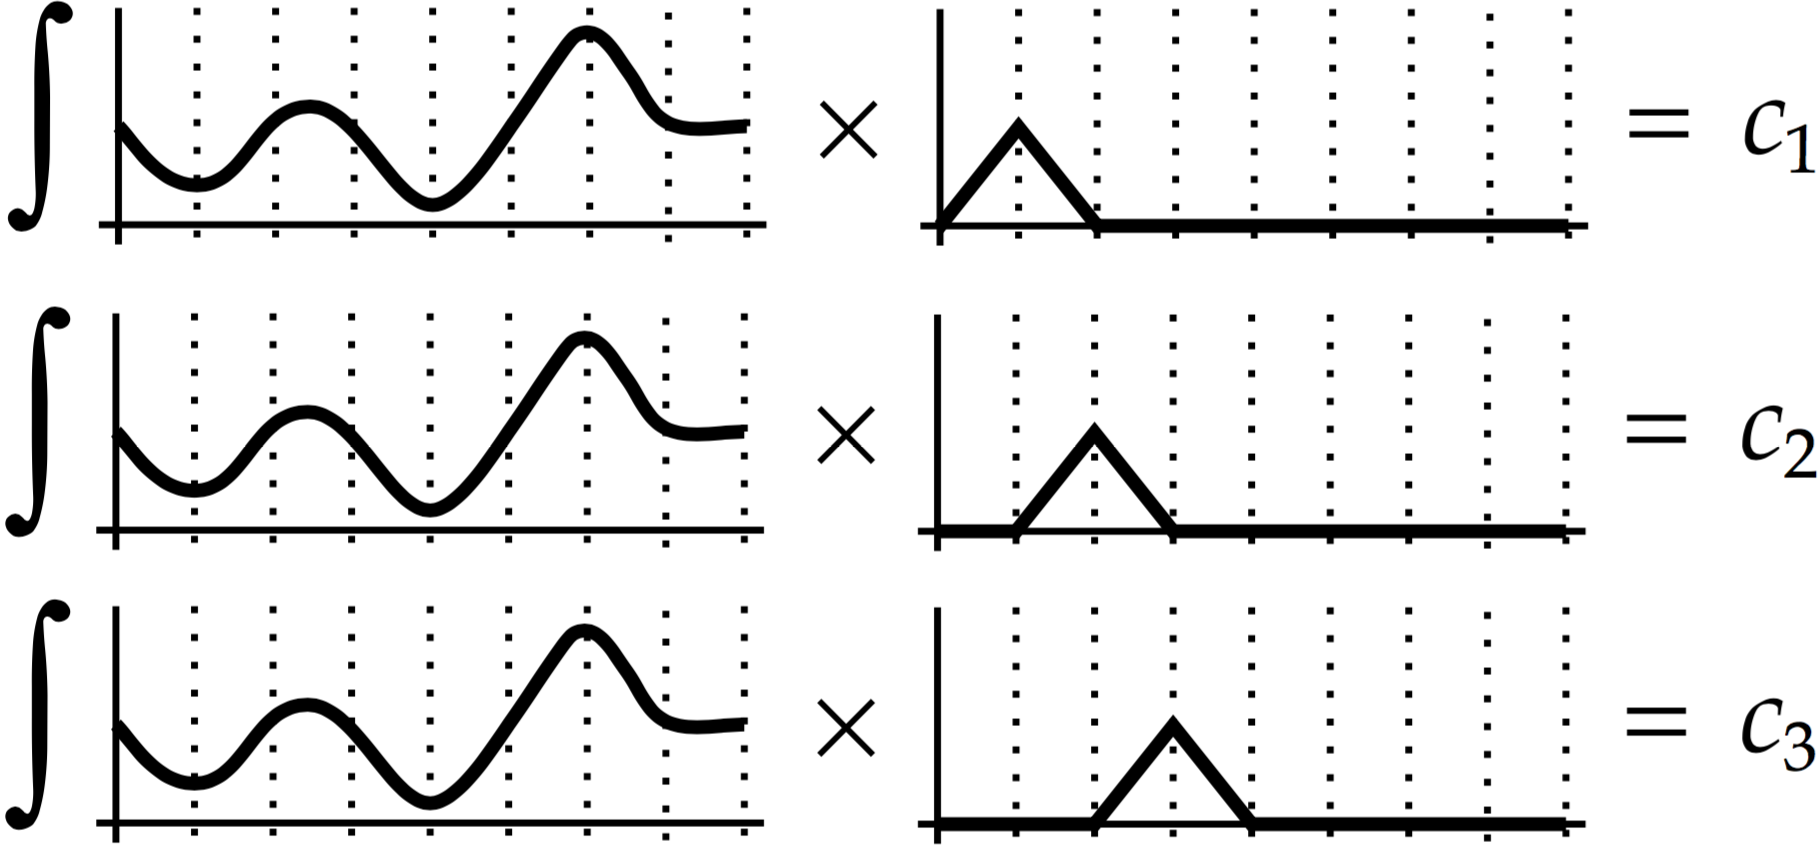
\includegraphics[width=\textwidth]{figures/prt/prt-1}
		\caption{投影}
	\end{subfigure}
		\begin{subfigure}[b]{0.49\textwidth}
		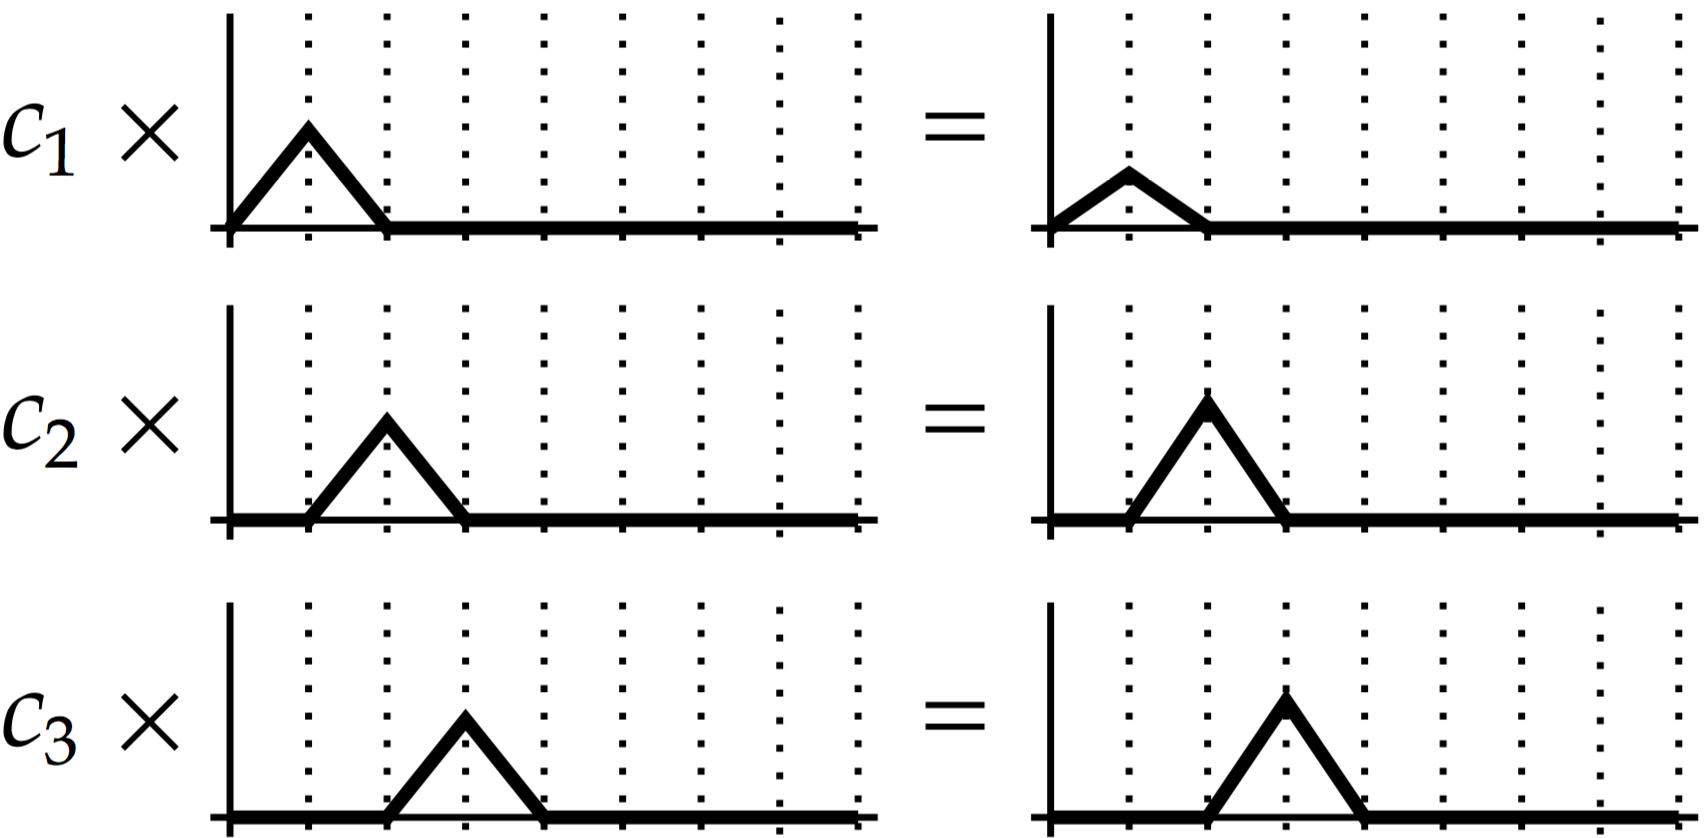
\includegraphics[width=\textwidth]{figures/prt/prt-2}
			\caption{重建}
	\end{subfigure}
	\caption{一种特殊的由线性分段函数组成的函数基,其每个基函数是一小段信号,它们可以被缩放并组合起来对原始函数形成近似,这个过程称为重建(b),决定每个基函数的缩放系数的过程被称为投影(a)。}
	\label{f:pl-projection-and-reconstruction}
\end{figure}

所以,如果已知一组基函数,则我们可以使用一个矢量来表述一个函数,该矢量的各个分量就是对于各个基函数的线性组合系数。给定一个定义在$T$上的函数$f(t)$以及一组基函数$B_i(t)$,该函数可以通过下面的积分被投影(projection)\mathindex{投影}{projection}(如图\ref{f:pl-projection-and-reconstruction}(a)所示)成系数(矢量)的形式:

\begin{equation}
	c_i=\int f(t)B_i(t)dt=:\langle f(t),B_i(t)\rangle
\end{equation}

然后,原始函数可以通过这些基函数与其对应系数乘积(如图\ref{f:pl-projection-and-reconstruction}(b)所示)的加和形式被重建(reconstruction)\mathindex{重建}{reconstruction},即:

\begin{equation}\label{e:pl-reconstruction}
	f(t)\approx\tilde{f}(t) =\sum_{i}^{N}c_iB_i(t)=\raisebox{-.5\height}{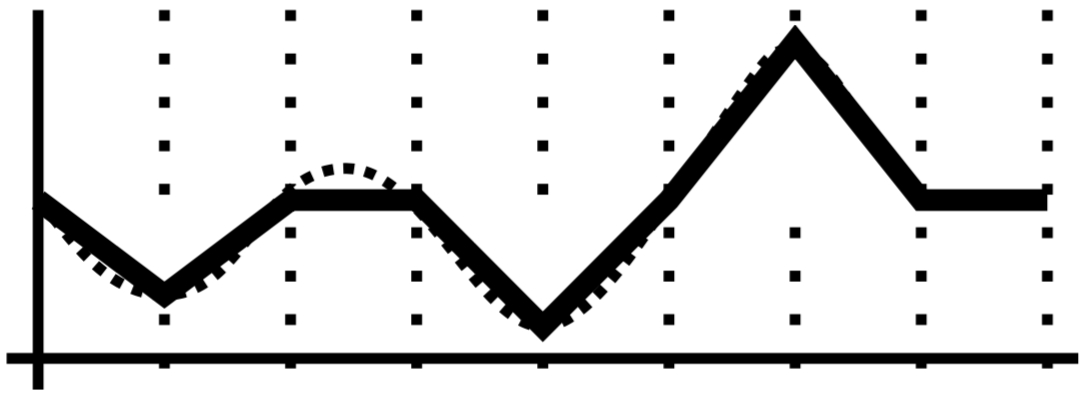
\includegraphics[width=0.25\textwidth]{figures/prt/prt-3}}
\end{equation}

这里$N$表示系数的数量,一个连续函数通常需要无穷多个基函数的线性组合才能完全被重建,当基函数的数量有限,或者$N$小于基函数的数量时,上述基函数的线性组合只是原始函数的一个近似,记为$\tilde{f}(t)$(见式\ref{e:pl-reconstruction})。

上面的例子使用了一系列线性(一次)函数作为基函数,它给出原始函数的一个分段线性近似。在工程上最常用的是使用一组相互正交的多项式作为函数基,正交多项式(orthogonal polynomials)\mathindex{正交多项式}{orthogonal polynomials}是一组具有一些有趣特性的多项式,即任意两个基函数之间都是相互正交的,所以当对任意两个基函数的乘积进行积分时,只有当两者完全相同时才会取得非零值,例如:

\begin{equation}
	\int_{-1}^{1}F_m(x)F_n(x)dx=\begin{cases}
		0 & \text{ for } n\neq m\\
		1 & \text{ for } n=m
	\end{cases}
\end{equation}

上式使用了更严格的限制:两个多项式乘积的积分必须返回0或者1,这些特定子集的基函数被称为标准正交基函数\footnote{注意正交(orthogonal)和标准正交(orthonormal)的区别,在欧几里得空间中,一个标准正交的基是指每个基矢量为单位矢量,并且相互正交。}(orthonormal basis functions)\mathindex{标准正交基函数}{orthonormal basis functions}。

有了上述的理论基础,我们便可以使用一个分量为各个基函数系数的矢量来表述或近似一个连续函数。很显然,每个表面处的光照传输是一个关于BRDF分布函数,可见性及几何项的函数,因此如果场景是静态的,那么该传输函数可以被存储为一个矢量而被重复使用,本节后面将讨论的一些性质将说明这些系数矢量怎样与动态的环境贴图组合在一起用于计算整个光照贡献。

然而,这里存在一个问题是,完整表述一个连续函数需要无限个系数,而光照传输发生于每个表面处,即每个表面位置都需要存储一个系数矢量,这显然面临巨大的存储和计算压力。为此,我们必须对每个表面点使用少量的系数对原函数进行近似,相对于由分段函数构成的基函数(如图\ref{f:pl-projection-and-reconstruction}所示),由多项式组成的基函数还具有另一种特征,不同阶的基函数能够表述原函数不同频率域的特征,阶数越高则保留的频率细节越多,但是需要的系数数量也越多,因此这给出一种可能,即使用少量的低阶多项式基函数来近似原函数的低频部分,这即是预计算辐射传输算法的核心思想。

本节首先讨论多项式基函数(如勒让德多项式)的一些特征,以及基于球面坐标系下的一种多项式基函数(即球谐函数),然后将在后面的内容中利用这些基函数的特征来实现预计算辐射传输算法。




\subsection{勒让德多项式}
工程中最感兴趣的一类多项式是勒让德多项式(Legendre polynomials)\mathindex{勒让德多项式}{Legendre polynomials},记为$P_l(x)$,其定义域为$x\in[-1,1]$,伴随勒让德多项式\footnote{有的数学文献又称其为连带勒让德多项式。}(associated Legendre Polynomials)\mathindex{伴随勒让德多项式}{associated Legendre Polynomials}$P^{m}_{l}(x)$ 和$P^{-m}_{l}(x)$是勒让德多项式的一般化或者说一般勒让德方程的解,其中$l$是一个非负整数,而$m=0,\cdots,l$,这些多项式返回实数(而一般的勒让德多项式返回复数)值。

对于给定正整数$m$,伴随勒让德多项式可以表述为一般非伴随勒让德多项式的形式,即:

\begin{equation}
\begin{aligned}
	p^{m}_{l}(x)&=(-1)^{m}(1-x^{2})^{m/2}\frac{d^{m}}{dx^{m}}P_l(x)\\
	&=\frac{(-1)^{m}}{2^{l}l!}(1-x^{2})^{m/2}\frac{d^{l+m}}{dx^{l+m}}(x^{2}-1)^{l}
\end{aligned}
\end{equation}

由此可以看出,参数$m$表示勒让德多项式导数的阶(order)\mathindex{阶}{order},如果$m=0$,则伴随勒让德多项式退化为多项式(相当于勒让德多项式的0阶导数)。

对于负整数$m$,其伴随勒让德多项式可以表述为:

\begin{equation}
	P_{l}^{-m}=(-1)^{m}\frac{(l-m)!}{(l+m)!}P^{m}_{l}(x)
\end{equation}

伴随勒让德多项式满足正交性,对于固定的$m$满足:

\begin{equation}
	\int^{1}_{-1}P^{m}_l(x) P^{m}_{l^{'}}(x)dx=\frac{2}{2l+1}\frac{(l+m)!}{(l-m)!}\delta_{ll^{'}}
\end{equation}

对于固定的$l$满足:

\begin{equation}
	\int^{1}_{-1}P^{m}_l(x)P^{m^{'}}_l(x)\frac{dx}{1-x^{2}}=\frac{(l+m)!}{m(l-m)!}\delta_{mm^{'}}
\end{equation}

那么伴随勒让德多项式的形式究竟是怎样的呢,这里不做推导,仅直接给出其形式。伴随勒让德多项式可以表述为下述的递归关系:

\begin{equation}\label{e:pl-associated-legendre-polynomials-1}
	(l-m)P^{m}_{l}(x)=x(2l-1)P^{m}_{l-1}(x)-(l+m-1)P^{m}_{l-2}(x)
\end{equation}

有了上述递归表述,就可以通过较小值的$l$推导出较大值$l$下同阶的伴随多项式。但是随着$l$的增大,伴随勒让德多项式的阶$m$也会增加(对于每一个参数$l$,$m=0,\cdots,l$),上式不足以推导出所有的伴随勒让德多项式,而下式给出了新增阶数的伴随勒让德多项式的递推关系:

\begin{equation}\label{e:pl-associated-legendre-polynomials-2}
\begin{aligned}
	P^{l}_l(x)&=(-1)^{l}(2l-1)!!(1-x^{2})^{l/2}\\
	P^{l}_{l+1}&=x(2l+1)P^{l}_l(x)
\end{aligned}
\end{equation}

有了式\ref{e:pl-associated-legendre-polynomials-1}和\ref{e:pl-associated-legendre-polynomials-2},便可以推导出任意参数$l$和$m$下的伴随勒让德多项式。例如以下是开头的6个伴随勒让德多项式:

\begin{equation}
\begin{aligned}
	P^{0}_0(x)&=1\\
	P^{0}_1(x)&=x\\
	P^{1}_1(x)&=-(1-x^{2})^{1/2}\\
	P^{0}_3(x)&=\frac{1}{2}(3x^{2}-1)\\
	P^{1}_2(x)&=-3x(1-x^{2})^{1/2}\\
	P^{2}_2(x)&=3(1-x^{2})\\
	&\cdots
\end{aligned}
\end{equation}

伴随勒让德多项式的另一个参数$l$的意义是什么呢,通过观察式\ref{e:pl-associated-legendre-polynomials-1}和\ref{e:pl-associated-legendre-polynomials-2},随着$l$的增加,变量$x$的指数次数会越来越大,实际上$l$表示了伴随勒让德多项式的次数(degree of a polynomial)\mathindex{多项式的次数}{degree of a polynomial},即多项式中所有单项式中指数次数和的最大值。由此也可以看出对于每一个固定的$l$,必须满足$m\leq l$,因为当$m>l$时(即导数的阶数大于多项式的次数),$P^{m}_l$的值始终为0。

\begin{figure}
\sidecaption
	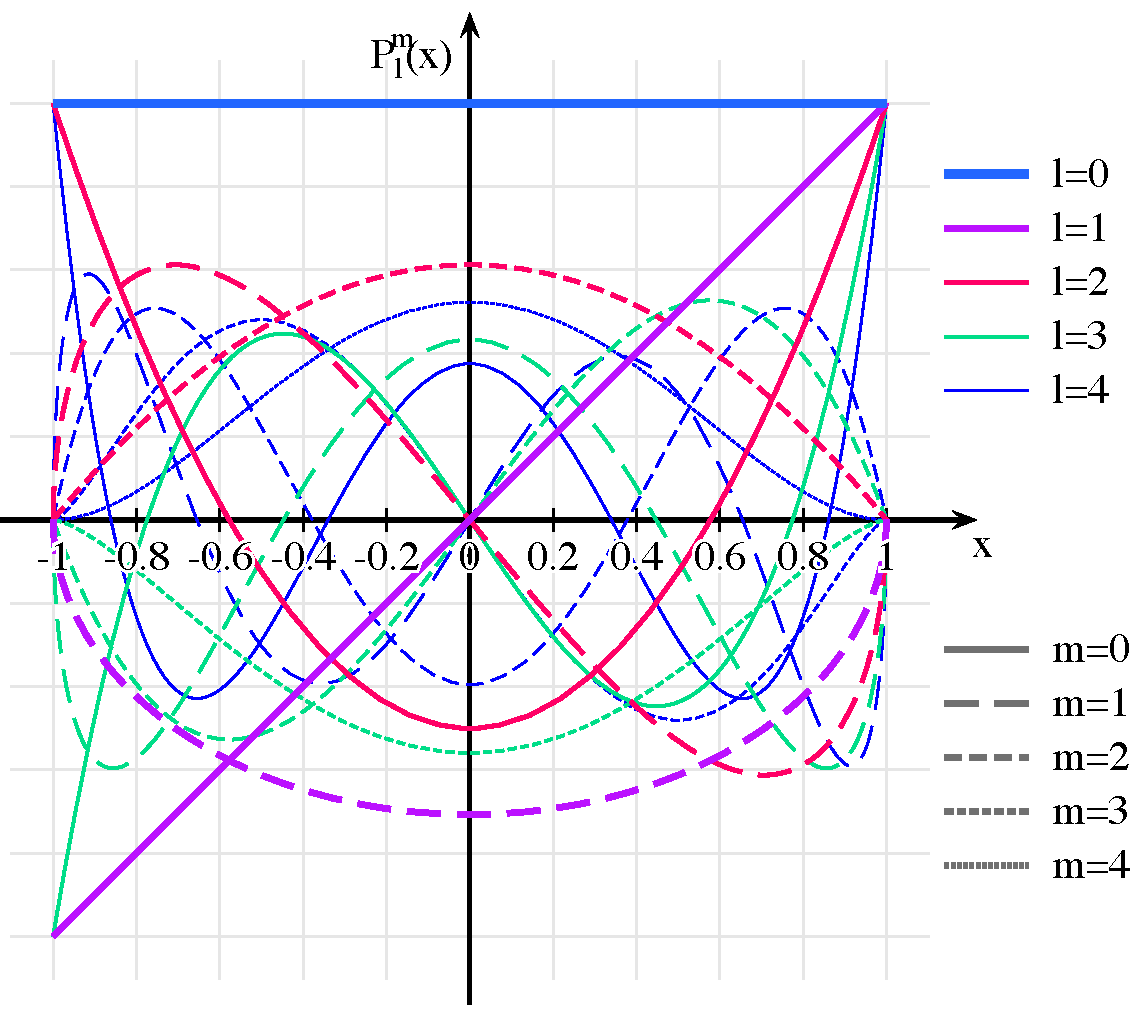
\includegraphics[width=0.65\textwidth]{figures/prt/associated-legendre-functions}
	\caption{伴随勒让德多项式的定义域为$[-1,1]$,右图展示了开头一些伴随勒让德多项式的图,注意这里没有包含阶数$m$为负数的多项式,所有多项式都被归一化到1,随着次数$l$的增大,多项式频率变得越来越高(图片来自Wikipedia,作者:Geek3)。}
	\label{f:pl-associated-legendre-functions}
\end{figure}

图\ref{f:pl-associated-legendre-functions}展示了开头一些伴随勒让德多项式的图,不难看出,随着次数$l$的增大,伴随勒让德多项式的频率变化变得原来越大,因此我们可以使用少数较低次数的伴随勒让德多项式来近似函数的低频部分。




\subsection{球谐函数}
满足拉普拉斯方程($\nabla^{2} f=0$,即为一个二阶连续可导函数)的函数称为谐函数(harmonic function)\mathindex{谐函数}{harmonic function},或者调和函数,球谐函数(spherical harmonics,SH)\mathindex{球谐函数}{spherical harmonics}则是将谐函数限制于球坐标系(spherical coordinates)\mathindex{球坐标系}{spherical coordinates}下的单位球面(unit sphere)上,即它忽略了球坐标系的半径$r$(因为其被固定于球面上),仅取其方向变化部分$\theta$和$\varphi$。因此正如同傅里叶级数(圆上的正弦和余弦函数)是一系列用于表示圆上的方向分布函数,球谐函数可以用来表述球面上的方向分布,例如表面的BRDF分布函数,环境贴图,光照传输,可见性分布等,这些都是仅与方向有关(而与位置无关)的函数。

球谐函数是定义于单位球面上的正交基,因此可以使用以下的参数化:

\begin{equation}
	s=(x,y,z)=(\sin\theta \cos\varphi,\sin\theta \sin\varphi,\cos\theta)
\end{equation}

来描述球谐函数,这里$s$就是单位球面上的一个位置。球谐函数一般使用符号$y$表述,其定义为:

\begin{equation}
	y^{m}_{l}(\theta,\varphi)=\begin{cases}
		\sqrt{2}K^{m}_{l}\cos(m\varphi)P^{m}_{l}(\cos\theta), &m>0\\
		\sqrt{2}K^{m}_{l}\sin(-m\varphi)P^{-m}_{l}(\cos\theta), &m<0\\
		K^{0}_{l}P^{0}_{l}(\cos\theta), & m=0
	\end{cases}
\end{equation}

这里$P$正是前面介绍的伴随勒让德多项式,而$K$仅仅是一个用以实现规则化的缩放系数,其值为:

\begin{equation}
	K^{m}_{l}=\sqrt{\frac{(2l+1)}{4\pi}\frac{(l-|m|)!}{(l+|m|)!}}
\end{equation}

同伴随勒让德多项式一样,我们使用不同的$l$和$m$(满足$-1\leq m\leq l$)的组合来获取所有的球谐函数,这是一个类似金字塔的数据结构,如图\ref{f:pl-sperical-harmonic}所示,为了简化表述,通常使用特定的顺序将其转换为一个平坦的一维矢量,所以我们又可以使用下面的序列定义球谐函数:

\begin{equation}\label{e:pl-harmonics-sequence}
	y^{m}_{l}(\theta,\varphi)=y_i(\theta,\varphi), \text{\quad\quad  其中\quad} i=l(l+1)+m
\end{equation}

在这个序列上,参数$l$将球谐函数分成不同的带(band),每个带内都是次数相同的多项式,给定参数$l$,其对应的带内包含$2l+1$个次数相同的球谐函数,如图\ref{f:pl-sperical-harmonic}所示。

\begin{figure}
\sidecaption
	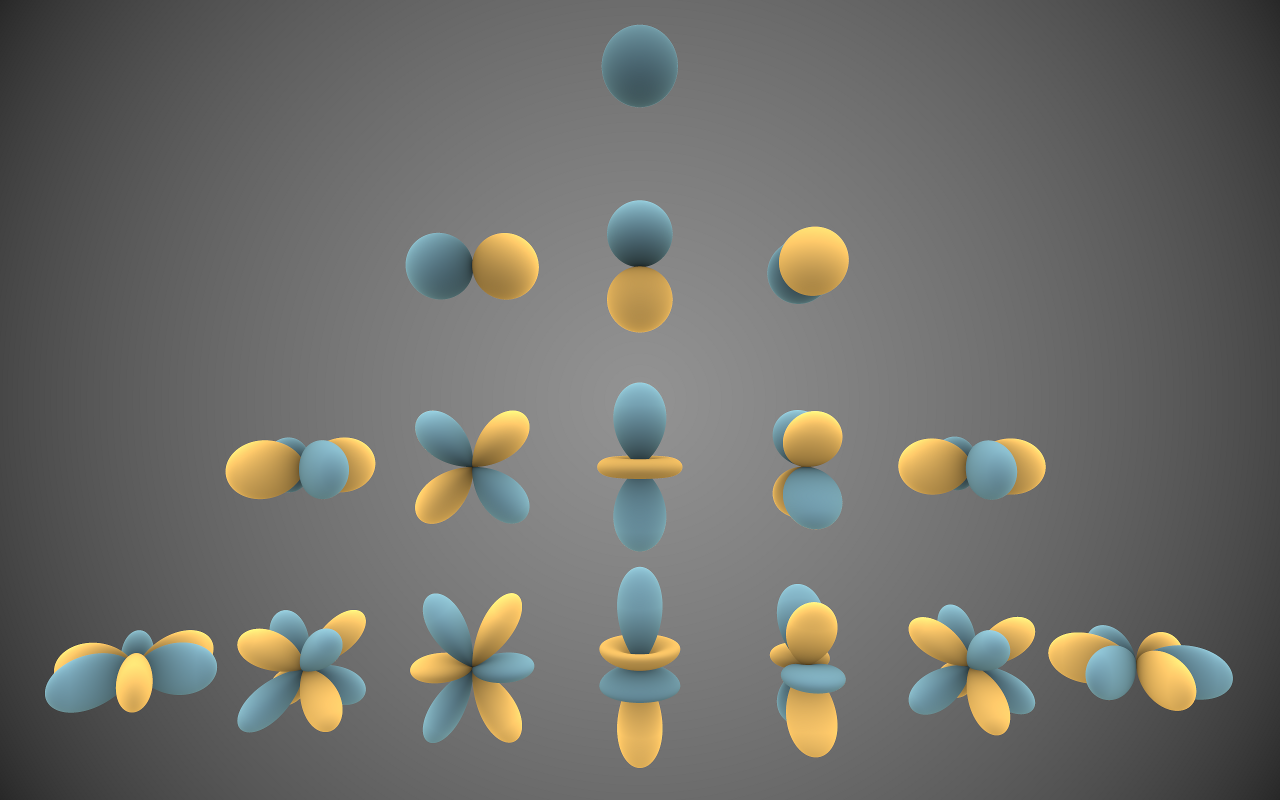
\includegraphics[width=0.65\textwidth]{figures/prt/prt-4}
	\caption{头4个带的球谐函数可视化图,蓝色部分表示函数取正值,黄色部分则表示负值区域,表面上的点到原点的距离指示方向$(\theta ,\phi )$上的函数值$y_{\ell }^{m}(\theta ,\phi )$(图片来自Wikipedia,作者:Inigo.quilez)。}
	\label{f:pl-sperical-harmonic}
\end{figure}

为了更直观的了解球谐函数的特征,我们希望像欧几里得空间的函数一样对其进行可视化(例如图\ref{f:pl-associated-legendre-functions}所示)。球谐函数可以被使用多种方法进行可视化,其中一种比较标准的方法是对单位球面执行扭曲变形操作,该操作对球面上每个点$y^{m}_l(\theta,\varphi)$沿其所在的方向$(\theta,\varphi)$进行缩放,使缩放后的表面上的每个点到原点的距离能够反映该球谐函数在该方向上的值$y^{m}_l(\theta,\varphi)$,同时用不同的颜色来区分球谐函数值的正负(蓝色为正,黄色为负),如图\ref{f:pl-sperical-harmonic}所示。从该图中也能够看出球谐函数的方向分布特征,每个带内的函数具有相似的频率变化,但是不同阶数的球谐函数具有不同的方向分布,以满足近似相似频率下函数的方向特征。




\subsubsection{投影和重建}
将一个球面函数投影为球谐函数系数的过程和一般的基函数投影是相同的,为了计算该投影系数,只需要将对原函数$f$与球谐函数$Y$的乘积进行积分即可:

\begin{equation}
	c_{l}^{m}=\int_{S}f(s)y^{m}_{l}(s)ds
\end{equation}

反之,为了重建对原函数的近似,对球谐函数按对应系数执行线性组合:

\begin{equation}
	\tilde{f}(s)=\sum^{n-1}_{l=0}\sum^{l}_{m=-1}c^{m}_{l}y^{m}_{l}(s)=\sum^{n^{2}}_{i=0}c_iy_i(s)
\end{equation}

可以看到,对原函数的$n$阶近似需要存储$n^{2}$个系数,同傅里叶级数一样,我们可以使用无限个球谐函数的系数来近似原始函数,所以,这里的每个重建实际上都只是一种近似,这称为带限近似(band-limited approximation),带限的过程是指将原始信息划分成各个频率分量,然后移除高于某个阈值的频率,这也是球谐函数中的参数$l$称为带的原因,它指的是频率带分布。

\begin{figure}
\begin{fullwidth}
	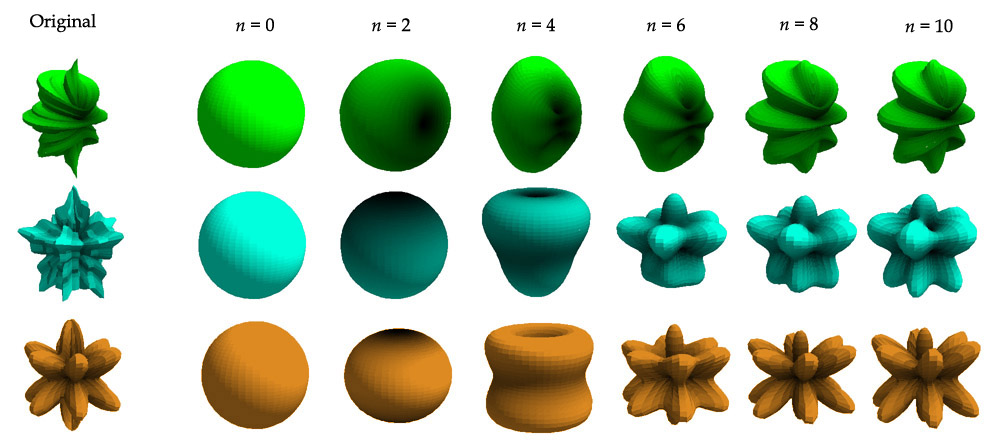
\includegraphics[width=1.0\thewidth]{figures/prt/prt-6-2}
	\caption{函数在球谐函数上的投影近似,随着球谐函数次数(带)$l$的提高,其对原始函数近似度也逐渐提高。(图片来自\cite{a:SphericalHarmonicLightingTheGrittyDetails}。}
	\label{f:pl-band-limited-approximation}
\end{fullwidth}
\end{figure}

图\ref{f:pl-band-limited-approximation}展示了对原始信号的不同带限近似,从左到右分别为常数,线性,二次,$\cdots$等近似,从中可以看到,随着带的增加,球谐函数能够更好地近似原始信号,因此对于低频函数,我们可以使用少量的系数就可以做到很好的近似。



\subsubsection{球谐函数的属性}
相较于其它基函数,球谐函数有一些有趣的特性使得其非常适合于解决光照传输中的一些问题,例如近似那些仅与方向相关的量。


\paragraph{基本属性}
首先,球谐函数之间不仅仅是相互正交(orthogonal)的,还是相互标准正交(orthonormal)的,这意味着如果我们对任意索引(使用式\ref{e:pl-harmonics-sequence}的表述)分别为$i$和$j$对应的球谐函数的乘积$y_iy_j$进行积分,其结果为1(如果$i=j$)或0(如果$i\neq j$)。

球谐函数的标准正交性提供了一种有用的属性,即对于给定的两个球面$S$上的函数$a$$b$,它们乘积的积分满足:

\begin{equation}\label{e:pl-dot-product}
	\int \tilde{a}(s)\tilde{b}(s)ds=\sum^{n^{2}}_{i=1}a_ib_i
\end{equation}

即经过旋转后的球谐函数的函数值保持不变。换句话说,两个带限函数乘积的积分被转化为它们各自投影系数的点积(dot product),这个属性在渲染方程中非常有用,我们可以将入射光照和传输函数均投影为球谐函数系数,而球谐函数的标准正交性保证了这些函数乘积的积分可以简单地计算为它们投影系数的内积。

其次,球谐函数还具有旋转不变性(rotational invariance)\mathindex{旋转不变性}{rotational invariance},即如果$Q$表示在球面$S$上的一个任意旋转,则对于函数$g(s)=f(Q(s))$,其投影为:

\begin{equation}
	\tilde{g}(s)=\tilde{f}(Q(s))
\end{equation}

换句话说,假设现有一个高频的环境光源$f$,并将其投影到球谐函数上得到一个低频的近似$\tilde{f}$,如果现在要对原始光源执行旋转操作$Q$,为了求出原始光源旋转过后的函数$g$的低频近似$\tilde{g}$的球谐函数系数,则我们可以通过直接对$\tilde{f}$的球谐函数系数执行一个线性变换来得到,这与首先对原始函数执行旋转$Q$得到$g$,然后再对$g$执行球谐函数投影得到$\tilde{g}$的效果是一样的,如图\ref{f:pl-sh-rotational-invariance}所示。

\begin{figure}
	\sidecaption
	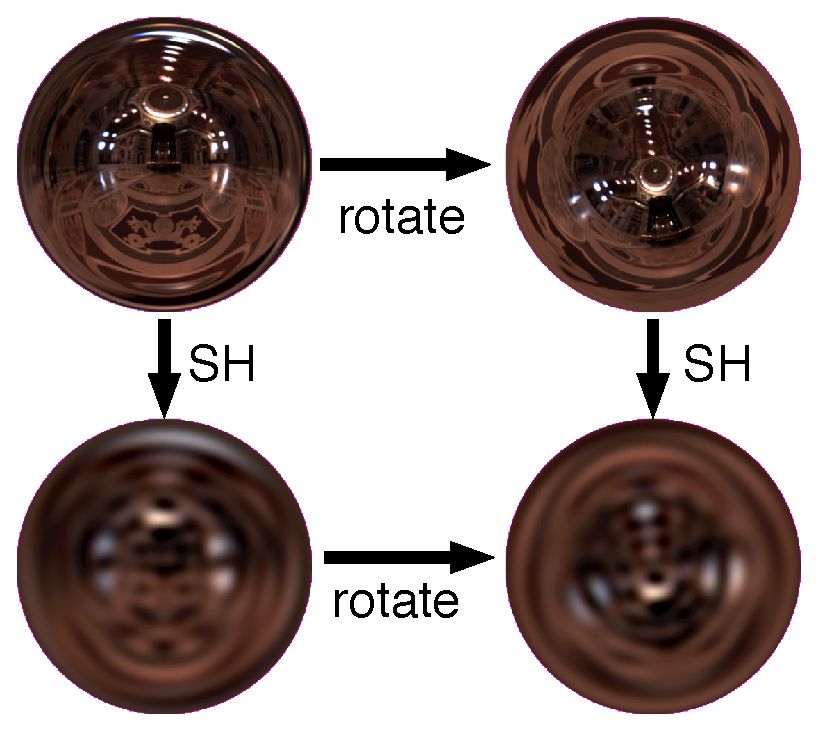
\includegraphics[width=0.42\textwidth]{figures/prt/sh-rotational-invariance}
	\caption{球谐函数具有旋转不变性,即对一个原始函数执行旋转再投影的操作(右上路径),可以直接通过对原始函数的投影系数执行一个线性变换操作(左下路径)来实现(图片来自\cite{a:StupidSphericalHarmonicsSHTricks})。}
	\label{f:pl-sh-rotational-invariance}
\end{figure}

这类似于傅里叶变换的移位不变性(shift invariance)\mathindex{移位不变性}{shift invariance},这意味着光源在旋转情况下是稳定的,因为不管光源发生什么样的旋转,我们只需要对光源执行一次采样操作以计算投影系数,然后任何旋转仅需要对这些系数构成的矢量执行线性变换即可,否则如果每次都需要对原始光源执行旋转,则需要重新计算投影系数,这就不得不对光源进行另一次采样,从而可能导致时间走样。

这个线性变换本质上是一个高维的旋转矩阵,我们将在第\ref{sec:pl-rotation}节介绍该矩阵的计算方法以及旋转的另外一些特性。




\paragraph{乘积的投影}
在前面的内容中,我们已经将整个光照计算分为光源(这里仅考虑与位置无关的环境贴图)和光照传输函数两部分,这两部分均可以看做是仅与方向有关的单位球面上的函数,因此可以分别使用一个球谐函数系数矢量进行近似。如果光照交互所处的表面是漫反射表面,则这两个球面函数乘积的积分是一个常数,因此该表面上光照的计算完全可以使用式\ref{e:pl-dot-product}所示的两个矢量的点乘表示,这两个矢量的分量对应于这两个方向分布函数在球面上的球谐函数投影系数,其中光源的投影系数可以动态调整,而表面上的投影系数可以预计算并缓存起来,以供每一帧执行光照计算,这样就能提高静态场景的计算效率,因为对于静态场景,其光照传输是不变的。

然而,当表面是光泽面时,光源和传输函数乘积的积分不再是一个常数积分值,因为摄像机从不同方向观察到的光照是不一样的,因此它是另一个方向分布函数,此时式\ref{e:pl-dot-product}不再适用,新的问题转换为对光源函数和传输函数的乘积(其结果为一个方向分布函数)的投影近似。即,设$c(s)=a(s)b(s)$为两个方向函数的乘积,我们需要对函数$c(s)$执行另一个投影近似。

根据投影的定义,其投影系数可表示为目标函数和球谐函数乘积的积分,因此函数$c(s)$的投影系数可由下式计算:

\begin{equation}
\begin{aligned}
	c_k=&\int y_k(s)c(s)ds\\
	   =&\int y_k(s)\Biggl(\sum^{n^{2}}_{i=0}a_iy_i(s)\Biggl)\Biggl(\sum^{n^{2}}_{j=0}b_jy_j(s)\Biggl)ds\\
	   =&\sum_{ij}\Gamma_{ijk}a_ib_j
\end{aligned}
\end{equation}

在上式的第二行中,$a(s)$和$b(s)$分别被其投影系数近似,$\Gamma$是一个三重积张量(triple product tensor)\mathindex{三重积张量}{triple product tensor}:

\begin{equation}
	\Gamma_{ijk}=\int y_i(s)y_j(s)y_k(s)ds
\end{equation}

$\Gamma_{ijk}$是一个3阶对称张量,这意味着如果在每个表面位置处存储完全的光照传输,这需要每个顶点存储一个三维矩阵,这显然会占用大量的存储资源。但这里我们可以把光源部分抽取出来,即假设光照传输(即$a(s)$)是已知(固定)的,而光源(即$b(s)$)是未知(可变)的,那么表面上每个位置处的光照传输就仅需要存储一个二维矩阵,该矩阵可以通过下式计算而出:

\begin{equation}
	\mathbf{M}_{ij}=\sum_k\Gamma_{ijk} a_i
\end{equation}

然后每个表面处的光照传输结果对应的方向函数$c(s)$的球谐函数系数为:

\begin{equation}
	c_i=\mathbf{M}_{ij}b_j
\end{equation}

通过上面的乘积投影(product projection)\myindex{乘积投影}{product projection}属性,我们就可以在预计算辐射度方法中处理光泽表面,其中函数$a(s)$表示如表面处的阴影遮挡分布,$b(s)$表示环境贴图光源,$c(s)=a(s)b(s)$表示出射光照的方向分布,我们通过在物体表面处存储一个传输矩阵$\mathbf{M}_{ij}$,然后动态改变光源$b(s)$,就可以按照上式很简单地计算出表面在各个方向的出射光照。




\paragraph{卷积的投影}
本书前面已经讨论过卷积的意义,它通常用来对原始信息进行平滑和过滤,在卷积计算中,一个核函数$h$分别作用于一个信号函数$f$的每一个位置处,其结果是一个更平滑的函数,记为$h*f$。

核函数同样可以用来平滑一个用球谐函数表述的方向分布函数,给定一个圆对称(circular symmetry)\myindex{圆对称}{circular symmetry}的核函数$h(z)$,通过对一个原始函数$f$执行卷积计算可以得到一个新的球谐函数,注意,这里核函数$h(z)$必须是圆对称的,即在垂直于$z$轴的平面上值相同,因此核函数可以只使用一个变量$z$表述,这样才能保证卷积的结果依然位于球面$S$上。

在球面上,卷积可以直接作用于方向函数的频率域(类似于傅里叶级数,球谐函数实际上就是方向函数的频率域),即

\begin{equation}\label{e:pl-sh-convolution}
	(h*f)^{m}_{l}=\sqrt{\frac{4\pi}{2l+1}}h^{0}_{l}f^{m}_{l}
\end{equation} 

也就是说,函数$f$的卷积就是该函数每个带$l$内的所有球谐函数系数$f^{m}_l$被核函数的$m=0$项$h^{0}_l$执行一个缩放操作,注意因为核函数是圆对称的,所以每个带$l$内仅仅只有$m=0$项(在后面将看到该项球谐函数称为带谐函数)具有非零值。该卷积属性提供了一种快速的方法用于计算环境贴图与余弦核函数$h(z) = \max(z,0)$的卷积计算,该操作可以得到一个辐射照度图(irradiance map)\myindex{辐射照度图}{irradiance map}。此外,卷积计算还可以用于对环境贴图执行预过滤操作以得到一个更平滑的环境贴图。
	
	

\subsection{球谐函数的旋转}\label{sec:pl-rotation}
在上面我们已经说明了球谐函数具有旋转不变性,但是并没有讨论怎样对球谐函数执行旋转操作。球谐函数的旋转操作对于光照渲染计算非常重要,例如每个物体表面的传输矢量(或矩阵)通常都是基于每个物体的局部坐标系的,而光源的球谐函数表述通常都是基于全局坐标系的,因此当它们在进行点积计算时,必须要将光源球谐函数旋转至每个物体的局部坐标系中,这个旋转操作发生于每个顶点甚至每个像素;并且,正如接下来的内容可知,球谐函数的旋转计算相对比较复杂,所以这里单独使用一个小节进行介绍。

对一个(系数)矢量执行一个线性变换的过程是什么呢,根据线性变换的定义,该操作实际上可以表述为一个旋转矩阵,使得旋转过后矢量的每个系数是原始系数的一个线性组合,即:

\begin{equation}\label{e:pl-linear-transform}
	g_i=\sum^{n^{2}}_j f_j R_{ij}
\end{equation}

由矩阵操作的定义可知,$R_{ij}$为一个$n^{2}\times n^{2}$的矩阵。然而根据群论(group theory)\mathindex{群论}{group theory}的知识,在该旋转矩阵中,带与带之间的系数并不相交,因此可以推断出旋转矩阵是一个基于块的稀疏对角矩阵,其中每个块的尺寸对应每个带内的阶数,即旋转后的每个球谐函数系数$g_i$仅来自于原始球谐函数中对应带内系数的线性变换。因此,即旋转矩阵具有下述的结构:

\begin{equation}\label{e:pl-sh-rotation-matrix}
	R_{SH}=\left[
	\centering
	\begin{array}{c|ccc|ccccc|c}
		\text{ 1 } & \text{ 0 } & \text{ 0 } & \text{ 0 } & \text{ 0 } & \text{ 0 } & \text{ 0 } & \text{ 0 } & \text{ 0 } & \cdots \\
		\hline
		0 & X & X & X & 0 & 0 & 0 & 0 & 0 & \cdots \\
		0 & X & X & X & 0 & 0 & 0 & 0 & 0 & \cdots \\
		0 & X & X & X & 0 & 0 & 0 & 0 & 0 & \cdots \\
		\hline
		0 & 0 & 0 & 0 & X & X & X & X & X & \cdots \\
		0 & 0 & 0 & 0 & X & X & X & X & X & \cdots \\
		0 & 0 & 0 & 0 & X & X & X & X & X & \cdots \\
		0 & 0 & 0 & 0 & X & X & X & X & X & \cdots \\
		0 & 0 & 0 & 0 & X & X & X & X & X & \cdots \\
		\hline
		\vdots & \vdots & \vdots & \vdots & \vdots & \vdots & \vdots & \vdots & \vdots & \ddots
	\end{array}
	\right]=\begin{bmatrix}
		1 & 0     & 0     & \cdots \\
		0 & R^{1} & 0     & \cdots \\
		0 & 0     & R^{2} & \cdots \\
		\vdots & \vdots & \vdots & \ddots 
	\end{bmatrix}
\end{equation}

如果已知一个该矩阵的显式表述,那么球谐函数旋转的操作就非常简单。然而实际上该旋转矩阵的计算非常复杂;并且由于它是一个关于旋转角度的函数,因此它必须在每次执行旋转操作的时候即时计算,因为此时我们才知道实际的旋转角度;此外,在实时渲染中由于每一帧都需要对每个顶点甚至每个像素执行旋转操作,所以单个旋转操作的计算效率非常重要。

以下我们首先简述旋转的计算方法,以及科学计算中球谐函数旋转的基本思路,然后介绍实时渲染中使用的快速计算方法。




\subsubsection{基本思路}
球谐函数旋转矩阵$R$(如式\ref{e:pl-sh-rotation-matrix})是一个$n^{2}\times n^{2}$高维矩阵,为了求出该高维旋转矩阵的数学形式,我们首先将目光转向传统3维笛卡尔坐标系下的旋转问题,因为球谐函数的旋转本质上也可以看做是一个3维空间的旋转问题。

根据欧拉旋转定理(Euler's rotation theorem)\mathindex{欧拉旋转定理}{Euler's rotation theorem},三维坐标系下的任意一个旋转(假设原始坐标系为$(x,y,z)$,旋转后的坐标系为$(X,Y,Z)$),都可以被分解为三个基本旋转的组合,这些基本旋转可能是围绕坐标轴的旋转,例如旋转组合$XYZ,ZYX$或者$ZYZ$等,其中每个基本旋转的角度按顺序来自于称为欧拉角$(\alpha,\beta,\gamma)$中的一个角度,例如对于$XYZ$组合,它首先围绕$X$轴旋转$\alpha$角度,接着围绕$Y$轴旋转$\beta$角度,最后围绕$Z$轴旋转$\gamma$角度。每个旋转组合定义一个$3\times 3$的旋转矩阵。

欧拉角(Euler angle)\mathindex{欧拉角}{Euler angle}是用于描述刚体在某个固定坐标系下的方向的三个角度,通常记为$(\alpha,\beta,\gamma)$,给定两个原点相同的坐标系以及特定的旋转组合,我们可以得出该旋转对应的欧拉角,这些欧拉角被用于描述一个$3\times 3$的旋转矩阵,进而被用于两个坐标内向量或点的旋转。

上述的3维旋转矩阵很容易被计算出来,它的每个元素是关于欧拉角的函数,为了区分,我们将其表述为$R_{3D}$,它是一个作用于传统3维笛卡尔坐标系的$3\times 3$矩阵,以区别于前面介绍的球谐函数旋转矩阵$R_{SH}$,它是一个作用于高维球谐函数坐标系的$n^{2}\times n^{2}$矩阵。

有了上述这些基础,群论\cite{a:GruppentheorieundihreAnwendungaufdieQuantenmechanikderAtomspektren}的知识指出,复数球谐函数的旋转矩阵的每个元素是关于上述3维旋转中元素的多项式,即是关于欧拉角的函数。\cite{a:RotationMatricesforRealSphericalHarmonicsDirectDeterminationbyRecursion}进一步指出实数球谐函数的旋转矩阵具有一种递推关系(recurrence relations)\mathindex{递推关系}{recurrence relations},使得可以更高效地计算实数球谐函数的旋转矩阵,该关系指出:

\begin{itemize}
	\item 对于固定的带(或次数)$l$,球谐函数旋转矩阵$R_{SH}$中的元素可以表述为原始3维旋转矩阵$R_{3D}$中元素的多项式,并且多项式的次数为$l$。
	\item 这些多项式可以以递归的形式被计算而出,即旋转矩阵$R^{l}_{SH}$中的元素可以表述为旋转矩阵$R^{l-1}_{SH}$中的元素与3维矩阵$R_{3D}$中元素的双线性关系(如式\ref{e:pl-sh-rotation-matrix})。
\end{itemize}

上述的递推关系使得我们可以计算出任意次数球谐函数的旋转矩阵,读者可以参考原论文中的详细递推关系。然而由于这样的计算成本对于实时渲染仍然是非常高的,因为实时渲染涉及每顶点甚至每像素的大量旋转计算,因此以下两节我们将介绍两种更高效的计算旋转矩阵的方法。




\subsubsection{ZXZXZ旋转}
上述的递推方法不对旋转矩阵的形式作出任何已知的假设,对于每一次旋转计算,它都从最低的次数开始递归计算,以构建出整个旋转矩阵的表达式。根据\cite{a:FastApproximationtoSphericalHarmonicRotation},递推方法构建旋转矩阵的计算复杂度约为$\mathcal{O}(l^{3})$,对球谐函数系数矢量执行旋转操作的复杂度也为$\mathcal{O}(l^{3})$。

\cite{a:FastArbitraryBRDFShadingforLowFrequencyLightingUsingSphericalHarmonics}发现,球谐函数围绕$z$轴的旋转具有比较简单的形式和计算量,因此提出一种称为$ZXZXZ$的旋转方法,该方法构建旋转矩阵的复杂度约为上述递推方法的一半,并且$ZXZXZ$方法直接推导出一个显式公式然后直接作用于系数矢量,因此省去了显式执行旋转变换的操作,进一步提高了旋转计算的效率。

该方法首先使用符号积分(symbolic integration)\mathindex{符号积分}{symbolic integration}表述出球谐函数旋转矩阵中每个元素的函数,即:

\begin{equation}\label{e:pl-sh-rotation-symbolic-form}
	\mathbf{M}_{ij}=\int_S y_i(\mathbf{R}s)y_i(s)ds
\end{equation}

上式具有什么意义呢?首先,我们需要解释一下什么是符号积分,符号积分跟传统的数值积分具有类似的含义,唯一的区别是数值积分计算的结果是一个确定的值,而符号积分的结果是一个函数,也就是说被积函数中包含除积分变量以外的自变量,可以理解为符号积分就是寻找不定积分的公式形式,因此上式\ref{e:pl-sh-rotation-symbolic-form}是一个函数,它给出球谐函数旋转矩阵$R_{SH}$中每个元素的形式;其次,那么旋转矩阵是关于谁的函数呢,在式\ref{e:pl-sh-rotation-symbolic-form}中,$R$是一个使用欧拉角表述的3维旋转矩阵,因此上述旋转矩阵元素就是关于欧拉角的函数;最后,为什么式\ref{e:pl-sh-rotation-symbolic-form}可以用来求球谐函数的旋转矩阵呢,这是因为$y_(Rs)$可以看做旋转后的球谐函数基,回想一个函数与某个基函数乘积的积分可以表述为该函数在该基函数上的投影,而坐标变换正是关于每个原始坐标轴(函数)在新坐标系下各个基函数上的投影,所以式\ref{e:pl-sh-rotation-symbolic-form}的积分可以用来表述球谐函数的旋转矩阵。

因此,如果能够直接求出式\ref{e:pl-sh-rotation-symbolic-form}的形式,则可以直接将其用于球谐函数系数矢量的旋转操作。例如,对于围绕$z$轴的旋转,其可以表述为以下的形式:

\begin{equation}
	\mathbf{M}_{ij}=\int^{2\pi}_0\int^{\pi}_0y_i(\theta,\varphi+\alpha)y_i(\theta,\varphi)\sin(\theta)d\theta d\varphi
\end{equation}

根据上式,我们可以得出围绕$z$轴的开头三个带的$9\times 9$旋转矩阵为:

\begin{equation}\label{e:pl-sh-rotation-z}
	Z_{\alpha}=\left[
	\centering
	\begin{array}{c|ccc|ccccc}
		\text{ 1 } & 0 & 0 & 0 & 0 & 0 & 0 & 0 & 0  \\
		\hline
		0 & \cos(\alpha) & 0 & \sin(\alpha) & 0 & 0 & 0 & 0 & 0  \\
		0 & 0 & 1 & 0 & 0 & 0 & 0 & 0 & 0 \\
		0 & -\sin(\alpha) & 0 & \cos(\alpha) & 0 & 0 & 0 & 0 & 0  \\
		\hline
		0 & 0 & 0 & 0 & \cos(2\alpha) & 0 & 0 & 0 & \sin(2\alpha)  \\
		0 & 0 & 0 & 0 & 0 & \cos(\alpha) & 0 & \sin(\alpha) & 0  \\
		0 & 0 & 0 & 0 & 0 & 0 & 1 & 0 & 0  \\
		0 & 0 & 0 & 0 & 0 & -\sin(\alpha) & 0 & \cos(\alpha) & 0  \\
		0 & 0 & 0 & 0 & -\sin(2\alpha) & 0 & 0 & 0 & \cos(2\alpha)  \\
	\end{array}
	\right]
\end{equation}

上述的矩阵形式也可以推广到次数更高的球谐函数,其中带$l$对应的项为$l\alpha$的正弦和余弦函数。从上述矩阵的结构也可以看出前面介绍的递推方法的思路,因为高次数的旋转矩阵对应的正余弦函数可以展开为低次数旋转矩阵对应的正余弦函数。

上述的矩阵$Z_{\alpha}$也揭示了另一个特征,即围绕$z$轴的旋转矩阵具有比较简洁而稀疏的形式,因此我们可以设想将整个旋转矩阵$R_{SH}$分解成$R_{\alpha}$与其它基本矩阵的组合,根据欧拉旋转定理,\cite{a:FastArbitraryBRDFShadingforLowFrequencyLightingUsingSphericalHarmonics}使用了$ZXZ$的旋转组合,这样三个基本旋转矩阵的其中两个都可以使用上述的围绕$z$轴的旋转矩阵$R_{\alpha}$,剩下的问题只需要计算出围绕$y$轴的旋转矩阵即可。\cite{a:FastArbitraryBRDFShadingforLowFrequencyLightingUsingSphericalHarmonics}进一步将该基础矩阵分解为三个矩阵的组合:首先围绕$x$轴旋转$90^{\circ}$,然后再围绕$z$轴旋转$\beta$角度,最后再围绕$x$轴旋转$-90^{\circ}$。其中,由于围绕$x$轴的两次旋转角度是固定的,因此这两个旋转矩阵可以被预存起来,即:

\begin{fullwidth}
\begin{equation}
\begin{aligned}
	X_{-90}=\left[
	\centering
	\begin{array}{c|ccc|ccccc}
		1 & 0 & 0 & 0 & 0 & 0 & 0 & 0 & 0  \\
		\hline
		0 & 0 & 1 & 0 & 0 & 0 & 0 & 0 & 0  \\
		0 & -1 & 0 & 0 & 0 & 0 & 0 & 0 & 0 \\
		0 & 0 & 0 & 1 & 0 & 0 & 0 & 0 & 0  \\
		\hline
		0 & 0 & 0 & 0 & 0 & 0 & 0 & 1 & 0  \\
		0 & 0 & 0 & 0 & 0 & -1 & 0 & 0 & 0  \\
		0 & 0 & 0 & 0 & 0 & 0 & -\frac{1}{2} & 0 & -\frac{\sqrt{3}}{2}  \\
		0 & 0 & 0 & 0 & -1 & 0 & 0 & 0 & 0  \\
		0 & 0 & 0 & 0 & 0 & 0 & -\frac{\sqrt{3}}{2} & 0 & \frac{1}{2}  \\
	\end{array}
	\right] && 
	X_{+90}=\left[
	\centering
	\begin{array}{c|ccc|ccccc}
		1 & 0 & 0 & 0 & 0 & 0 & 0 & 0 & 0  \\
		\hline
		0 & 0 & -1 & 0 & 0 & 0 & 0 & 0 & 0  \\
		0 & 1 & 0 & 0 & 0 & 0 & 0 & 0 & 0 \\
		0 & 0 & 0 & 1 & 0 & 0 & 0 & 0 & 0  \\
		\hline
		0 & 0 & 0 & 0 & 0 & 0 & 0 & -1 & 0  \\
		0 & 0 & 0 & 0 & 0 & -1 & 0 & 0 & 0  \\
		0 & 0 & 0 & 0 & 0 & 0 & -\frac{1}{2} & 0 & -\frac{\sqrt{3}}{2}  \\
		0 & 0 & 0 & 0 & -1 & 0 & 0 & 0 & 0  \\
		0 & 0 & 0 & 0 & 0 & 0 & -\frac{\sqrt{3}}{2} & 0 & \frac{1}{2}  \\
	\end{array}
	\right]
\end{aligned}
\end{equation}
\end{fullwidth}

根据上述过程,原始的旋转矩阵被分解为以下ZXZXZ的旋转矩阵的组合:

\begin{equation}
	R_{SH}(\alpha,\beta,\gamma)=Z_{\gamma}X_{-90}Z_{\beta}X_{+90}Z_{\alpha}
\end{equation}

上式涉及到4个$9\times 9$矩阵的相乘计算,我们可以进一步将这些矩阵的相乘转变为一个显式的旋转矩阵,并且其中的每个包含欧拉角的三角函数的矩阵元素可以表述原始$R_{3D}$中元素的多项式。将该矩阵直接作用于球谐函数系数矢量,这相对于递推方法省略了显式构建的过程(由本节开头的内容可知,仅该显式矩阵的构建复杂度都为$\mathcal{O}(n^{3})$)。

$ZXZXZX$方法虽然简单,但是它仅适用于次数比较小的球谐函数的旋转,例如$l\leq 6$,对于较高次数的球谐函数,由于围绕$y$轴计算成本增加很快,因此其效率会低于递推方法,但是这对于实时渲染来说基本上已经足够。



\subsubsection{快速近似法}
$ZXZXZ$方法中的缺点在于围绕$y$轴的计算很耗时,\cite{a:FastApproximationtoSphericalHarmonicRotation}在此基础上对$R_y$提出一种使用低阶泰勒展开(Taylor expansion)\mathindex{泰勒展开}{Taylor expansion}的近似方法,该方法的矩阵分解可以表述为
	$R=R_z(\alpha)R_y(\beta)R_z(\gamma)$,其中围绕$z$轴的$R_z(\alpha)$和$R_z(\gamma)$采样上节介绍的方法进行计算。

为了计算$R_y(\beta)$,我们首先使用二阶泰勒公式将其展开,即:

\begin{equation}\label{e:pl-sh-rotation-2-taylor}
	\mathbf{R}_y(\beta)\approx\mathbf{I}+\beta\frac{d\mathbf{R}_y}{d\beta}(0)+\frac{\beta^{2}}{2}\frac{d^{2}\mathbf{R}_y}{d\beta}(0)
\end{equation}

这里$\mathbf{I}$为单位矩阵,上述$\mathbf{R}_y$的一阶和二阶导数如式\ref{e:pl-sh-rotation-taylor}所示,它们是根据前面介绍的递推方法推导而来,\cite{a:FastApproximationtoSphericalHarmonicRotation}的附录A包含了其推导过程。注意这里旋转矩阵$\mathbf{R}$的右上标表示的是球谐函数的次数(或带数)$l$,所以$\mathbf{R}^{l}_y$及其导数均是一个$2l+1\times 2l+1$的矩阵。

观察式\ref{e:pl-sh-rotation-taylor}可以看出,$\mathbf{R}_y$的一阶导数矩阵$\frac{d\mathbf{R}_y}{d\beta}(0)$(式\ref{e:pl-sh-rotation-taylor}的左边一列)仅仅在上下两个副对角线上具有非零值(如图\ref{f:pl-15-taylor}(b)所示),而$\mathbf{R}_y$的二阶导数矩阵$\frac{d^{2}\mathbf{R}_y}{d\beta^{2}}(0)$(式\ref{e:pl-sh-rotation-taylor}的右边一列)仅仅在主对角线,以及高于上副对角线和低于下副对角线的两个对角线上具有非零值(如图\ref{f:pl-15-taylor}(c)所示),因此$\mathbf{R}_y$的二阶泰勒展开是一个非常稀疏的矩阵(如图\ref{f:pl-15-taylor}(d)所示),并且我们知道哪些元素具有非零值,所以仅仅需要构建这部分矩阵元素即可。

\begin{figure}
\begin{fullwidth}
	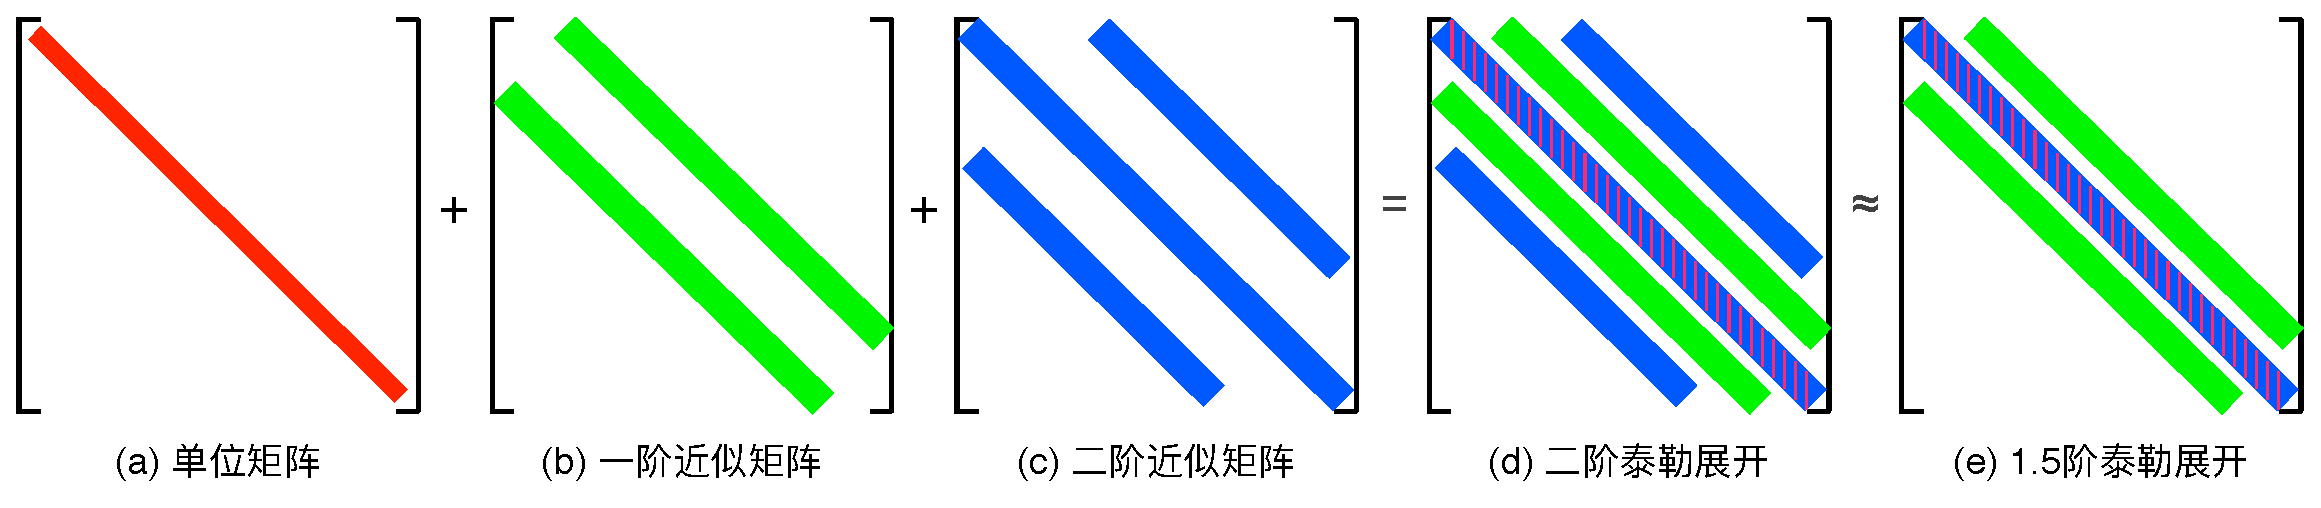
\includegraphics[width=1.0\thewidth]{figures/prt/15-taylor}
	\caption{围绕$y$轴的球谐函数旋转矩阵$\mathbf{R}_y$的二阶泰勒展开及其各项的矩阵,(a),(b)和(c)分别对应式\ref{e:pl-sh-rotation-2-taylor}中的单位矩阵,一阶导数矩阵和二阶导数矩阵,由于二阶导数矩阵(d)的非主对角线项具有对整个近似具有较小的影响,因此这些元素被忽略,而形成一个1.5阶的泰勒近似(e)。}
	\label{f:pl-15-taylor}
\end{fullwidth}
\end{figure}

在实践中,\cite{a:FastApproximationtoSphericalHarmonicRotation}发现$\mathbf{R}_y$的二阶泰勒展开项中的非主对角线(即高于上副对角线和低于下副对角线的两个对角线)上的元素对整个近似的影响很小,因此这些对象性上的元素被忽略,剩下的整个二阶泰勒近似矩阵仅包含主对角线和上下两个副对角线上的元素,这称之为一个1.5阶泰勒近似,如图\ref{f:pl-15-taylor}(e)所示,相比式\ref{e:pl-sh-rotation-2-taylor},它的精确度只有一点点损失,但是减少了更多的计算量。

该近似方法的计算复杂度为$\mathbf{O}(n^{2})$,据\cite{a:FastApproximationtoSphericalHarmonicRotation}说明,该方法比$ZXZXZ$方法的性能快约$4\sim 5$倍,这使得该方法甚至可以用于实时的每像素计算中。然而由于使用了泰勒近似,因此该方法仅适用于比较小的旋转角度,但是这种限制在实时渲染中影响较小,我们会在后面的例子中给予说明,并且即使某些少量的旋转角度大于一定的误差范围,我们可以对这少部分的旋转计算转换为使用前面介绍的$ZXZXZ$方法。

\begin{figure}
\begin{equation}\label{e:pl-sh-rotation-taylor}
\rotatebox{90}{$
\begin{aligned}
	\frac{dR_Y}{d\beta}(0)&=\begin{pmatrix}
		0          & \mathbf{0}                 & \mathbf{0}                 & \mathbf{0}                 & \cdots \\
		\mathbf{0} & \frac{dR^{1}_Y}{d\beta}(0) & \mathbf{0}                 & \mathbf{0}                 & \cdots \\
		\mathbf{0} & \mathbf{0}                 & \frac{dR^{2}_Y}{d\beta}(0) & \mathbf{0}                 & \cdots \\
		\mathbf{0} & \mathbf{0}                 & \mathbf{0}                 & \frac{dR^{3}_Y}{d\beta}(0) & \cdots \\
		\vdots     & \vdots                     & \vdots                     & \vdots                     & \ddots
	\end{pmatrix} & \frac{d^{2}R_Y}{d\beta^{2}}(0)&=\begin{pmatrix}
		0          & \mathbf{0}                         & \mathbf{0}                         & \mathbf{0}                         & \cdots \\
		\mathbf{0} & \frac{d^{2}R^{1}_Y}{d\beta^{2}}(0) & \mathbf{0}                         & \mathbf{0}                         & \cdots \\
		\mathbf{0} & \mathbf{0}                         & \frac{d^{2}R^{2}_Y}{d\beta^{2}}(0) & \mathbf{0}                         & \cdots \\
		\mathbf{0} & \mathbf{0}                         & \mathbf{0}                         & \frac{d^{2}R^{3}_Y}{d\beta^{2}}(0) & \cdots \\
		\vdots     & \vdots                             & \vdots                             & \vdots                             & \ddots
	\end{pmatrix}\\
	\text{其中:} && \text{其中:}\\
	\frac{dR^{1}_Y}{d\beta}(0)&=\begin{pmatrix}
		0 & 0 & 0\\
		0 & 0 & -1\\
		0 & 1 & 0
	\end{pmatrix} & \frac{d^{2}R^{1}_Y}{d\beta^{2}}(0)&=\begin{pmatrix}
		0 & 0  & 0\\
		0 & -1 & 0\\
		0 & 1  & -1
	\end{pmatrix}\\
	\frac{dR^{2}_Y}{d\beta}(0)&=\begin{pmatrix}
		0  & 1 & 0    & 0     & 0\\
		-1 & 0 & 0    & 0     & 0\\
		0  & 0 & 0    & -1.73 & 0\\
		0  & 0 & 1.73 & 0     & -1\\ q
		0  & 0 & 0    & 1     & 0
	\end{pmatrix} & \frac{d^{2}R^{2}_Y}{d\beta^{2}}(0)&=\begin{pmatrix}
		-1 & 0  & 0    & 0  & 0\\
		0  & -1 & 0    & 0  & 0\\
		0  & 0  & -3   & 0  & 1.73\\
		0  & 0  & 0    & -4 & 0\\
		0  & 0  & 1.73 & 0  & -1
	\end{pmatrix}\\
	\frac{dR^{3}_Y}{d\beta}(0)&=\begin{pmatrix}
		0     & 1.22  & 0    & 0    & 0     & 0     & 0\\
		-1.22 & 0     & 1.58 & 0    & 0     & 0     & 0\\
		0     & -1.58 & 0    & 0    & 0     & 0     & 0\\
		0     & 0     & 0    & 0    & -2.45 & 0     & 0\\
		0     & 0     & 0    & 2.45 & 0     & -1.58 & 0\\
		0     & 0     & 0    & 0    & 1.58  & 0     &-1.22\\
		0     & 0     & 0    & 0    & 0     & 1.22  & 0
 	\end{pmatrix} & 
 	\frac{d^{2}R^{3}_Y}{d\beta^{2}}(0)&=\begin{pmatrix}
		-1.5 & 0  & 1.94 & 0    & 0    & 0    & 0\\
		0    & -4 & 0    & 0    & 0    & 0    & 0\\
		1.94 & 0  & -2.5 & 0    & 0    & 0    & 0\\
		0    & 0  & 0    & -6   & 0    & 3.78 & 0\\
		0    & 0  & 0    & 0    & -8.5 & 0    & 1.94\\
		0    & 0  & 0    & 3.78 & 0    & -4   & 0\\
		0    & 0  & 0    & 0    & 1.94 & 0    & -1.5
 	\end{pmatrix} 
\end{aligned}$}
\end{equation}
\end{figure}




\subsubsection{带谐函数}
如果函数$f$是关于$z$轴圆对称的,则它的投影中仅包含$m=0$的球谐函数,这样的球谐函数也称为带谐函数(zonal harmonics,ZH),如图\ref{f:pl-sperical-harmonic}的中间一列所示。广义的带谐函数是指在单位圆上围绕任意一个对称轴圆对称的方向函数,例如大部分参与介质中的相位函数(phase function)\mathindex{相位函数}{phase function}都是圆对称的方向函数。所有的带谐函数都可以由围绕$z$轴的带谐函数旋转而来,为了便于描述,以下我们仅称围绕$z$轴圆对称的球谐函数为(狭义的)带谐函数,而本节的目标就是要讨论带谐函数的旋转。

相对于普通球谐函数,带谐函数的旋转操作要简单得多,因为带谐函数在每个带中只取一个基函数($m=0$),所以式\ref{e:pl-sh-rotation-matrix}中的每个带内仅包含中间的一列取非零值,既具有如下的矩阵结构:

\begin{equation}\label{e:pl-zonal-rotation-matrix}
	R=\left[
	\centering
	\begin{array}{c|ccc|ccccc|c}
		\text{ 1 } & \text{ 0 } & \text{ 0 } & \text{ 0 } & \text{ 0 } & \text{ 0 } & \text{ 0 } & \text{ 0 } & \text{ 0 } & \cdots \\
		\hline
		0 & 0 & X & 0 & 0 & 0 & 0 & 0 & 0 & \cdots \\
		0 & 0 & X & 0 & 0 & 0 & 0 & 0 & 0 & \cdots \\
		0 & 0 & X & 0 & 0 & 0 & 0 & 0 & 0 & \cdots \\
		\hline
		0 & 0 & 0 & 0 & 0 & 0 & X & 0 & 0 & \cdots \\
		0 & 0 & 0 & 0 & 0 & 0 & X & 0 & 0 & \cdots \\
		0 & 0 & 0 & 0 & 0 & 0 & X & 0 & 0 & \cdots \\
		0 & 0 & 0 & 0 & 0 & 0 & X & 0 & 0 & \cdots \\
		0 & 0 & 0 & 0 & 0 & 0 & X & 0 & 0 & \cdots \\
		\hline
		\vdots & \vdots & \vdots & \vdots & \vdots & \vdots & \vdots & \vdots & \vdots & \ddots
	\end{array}
	\right]
\end{equation}

那么应该怎样(使用简单的方法)计算出上述的旋转矩阵呢?即我们的目标是要计算出上述矩阵中非零项的列中每个元素的值,可以记为$C_{lm}$。为了计算旋转矩阵中的元素值,可以考虑对一个位置$z=(0,0,1)$处的脉冲函数$\delta(s)$执行旋转,由于脉冲函数具有确定(且简单)的表述形式,我们可以借此来计算旋转矩阵的元素值$C_{lm}$,然后将该旋转矩阵运用于一般的带谐函数的旋转。

首先根据投影的定义可计算出位置$(0,0,1)$处的脉冲函数的投影系数为:

\begin{equation}\label{e:pl-delta-sh-coefficients}
	\delta_l=\int\delta(s)y^{0}_{l}(s)ds=y^{0}_{l}(z)=\sqrt{\frac{2l+1}{4\pi}}
\end{equation}

在上式中,由于带谐函数的投影仅包含$m=0$项,所以这里系数$\delta_l$仅与带$l$有关;其次,由于脉冲函数仅在$(0,0,1)$处取值且为1,所以上述的投影积分值即为球谐函数$y^{0}_l(s)$在$s=z=(0,0,1)$处的值,该脉冲函数的带谐函数近似如图\ref{f:pl-zonal-rotation}(a)所示。

现在我们对脉冲函数$\delta(s)$执行一个旋转操作,使其旋转到任意指定方向$z^{'}$,得到$\hat{\delta}(s)$,如图\ref{f:pl-zonal-rotation}(b)所示,根据和式\ref{e:pl-delta-sh-coefficients}类似的方法可以得出$\hat{\delta}(s)$的投影系数为:

\begin{equation}
	\hat{\delta}^{m}_l=\int\hat{\delta}(s)y^{m}_{l}(s)ds=y^{m}_{l}(z^{'})
\end{equation}

注意这里$z^{'}$表示一个已知的确定值。由于旋转后的函数不再是关于$z$轴圆对称的(如图\ref{f:pl-zonal-rotation}(b)所示),所以它会投影到每个带内的各个$m$值对应的球谐函数上,因此其系数同时与$m$和$l$相关。

\begin{figure}
	\sidecaption
	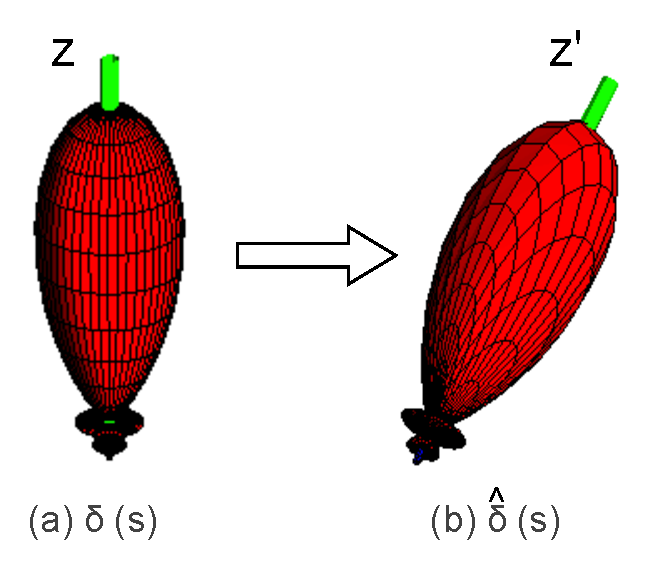
\includegraphics[width=0.47\textwidth]{figures/prt/zonal-rotation}
	\caption{(a)为单位球面上位置$(0,0,1)$处的脉冲函数的球谐函数近似,其中$l=6$,(b)为其旋转到方向$z^{'}$后的近似。由于脉冲函数的表述比较简单,因此可以用来计算带谐函数的旋转矩阵(图片来自\cite{a:LocalDeformablePrecomputedRadianceTransfer})。}
	\label{f:pl-zonal-rotation}
\end{figure}

根据旋转不变性,对系数$\delta_l$执行旋转操作后的值等于系数$\hat{\delta}^{m}_l$,可以得到:

\begin{equation}
	C_{lm}\delta_l=\hat{\delta}^{m}_{l}=y^{m}_{l}(z^{'})
\end{equation}

由上式可以计算出旋转矩阵中的元素的值为:

\begin{equation}
	C_{lm}=y^{m}_l(z^{'})/\delta_l=\sqrt{\frac{4\pi}{2l+1}} y^{m}_l(z^{'})
\end{equation}

由此我们便计算出了带谐函数的旋转矩阵中每个元素的值,进而可以将该旋转矩阵运用于任意由$z$旋转到$z^{'}$方向的带谐函数。一般地,假设$g(s)$为关于$z$轴圆对称的带谐函数,将其旋转至$s^{*}$方向得到$\hat{g}(s)$,如果已知$g(s)$的投影系数为$g_l$,则旋转至$s^{*}$方向后的函数$\hat{g}(s)$的的投影系数为:

\begin{equation}
	\hat{g}^{m}_l=\sqrt{\frac{4\pi}{2l+1}} y^{m}_l(s^{*}) g_l
\end{equation}

将上式和式\ref{e:pl-sh-convolution}进行对比可以发现,对带谐函数执行旋转的操作,等效于带谐函数$g(s)$与一个方向$s^{*}$处的脉冲函数$\delta(s)$的卷积(该脉冲函数的投影系数为$y^{m}_l(s^{*})$)。




\section{基于图像的光照技术}\label{sec:pl-ibl}
基于图像的光照(image-based lighting,IBL)\myindex{基于图像的光照}{image-based lighting}技术,主要是指将某种形式的光照度量(例如辐射照度或辐射亮度等)存储为图片的格式,然后在渲染时相应部分的光照计算被转化为对纹理数据的查询或读取,这可以大大加速光照的计算,被广泛运用于离线和实时渲染中。

当前大部分基于图像的光照技术主要都是基于环境映射(environment mapping)\myindex{环境映射}{environment mapping}的,环境映射又称为反射映射(reflection mapping)\myindex{反射映射}{reflection mapping},它最早由\cite{a:Textureandreflectionincomputergeneratedimages}提出,主要用于加速镜面曲面对周围环境的反射计算。传统的镜面反射光照的计算需要对镜面曲面上的每一个点分别执行光照计算,也就是说曲面上的入射光照分布是随着着色位置的变化而变化的,这就使得镜面反射光照的计算很难达到实时要求。然而,如果假设周围环境距离当前着色物体比较远,以至于物体表面着色位置的变化对光照的影响相对于物体与环境的距离是可以忽略不计的,这时的环境光照也就可以近似认为是与着色位置无关的,而仅与方向有关,所以我们可以将整个周围的环境光照缓存到一张纹理当中,然后通过一个入射方向作为索引对纹理数据进行读取,此时环境光照的计算转变为对一个纹理的查询操作(当然这也忽略了局部物体之间的遮挡关系),这可以大大加速环境光照的计算。

\begin{figure}
	\sidecaption
	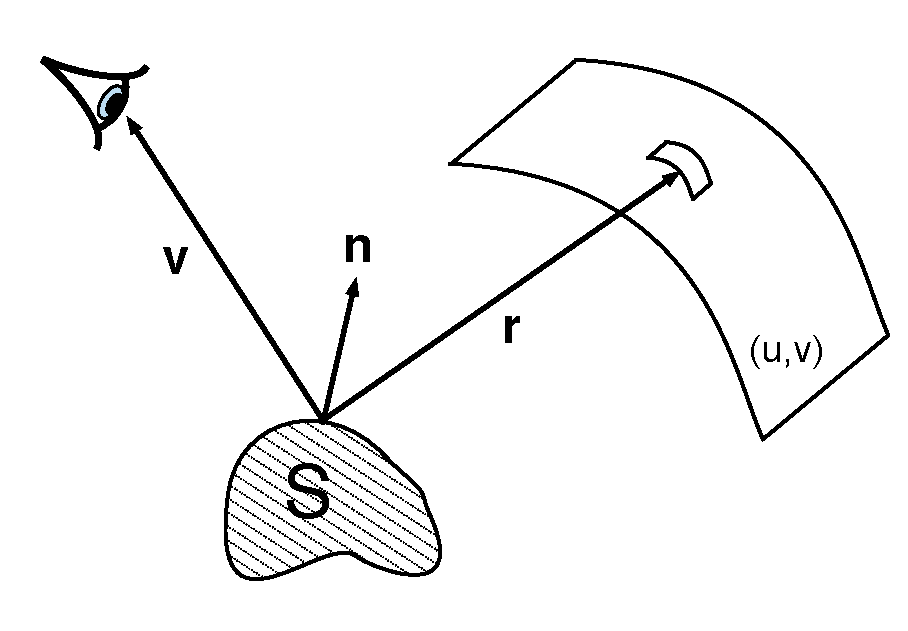
\includegraphics[width=0.55\textwidth]{figures/pl/environment-mapping}
	\caption{反射映射的基本概念图,图中物体$S$为镜面曲面,$\mathbf{n},\mathbf{v}$和$\mathbf{r}$分别为着色点处的法线,观察方向和入射方向,它们的关系可由反射定律得出,右上角的曲面表示一个环境贴图,其中入射方向$r$首先被映射为一个纹理坐标$(u,v)$,然后用于直接从环境贴图中读取入射光照。}
	\label{f:pl-environment-mappling}
\end{figure}

图\ref{f:pl-environment-mappling}演示了环境映射的基本概念,对于镜面曲面$S$,它与光的交互遵循反射定律,因此对于给定法线$\mathbf{n}$和观察方向$\mathbf{v}$,其入射方向$\mathbf{r}$为:

\begin{equation}
\mathbf{r}=2(\mathbf{n}\cdot\mathbf{v})\mathbf{n}-\mathbf{v}
\end{equation}

环境贴图中存储的是入射光照的方向分布,因此上式计算出的入射方向$\mathbf{r}$可以用于对环境贴图的查询操作。但是要知道怎么对环境贴图按方向进行查询(或索引),我们需要知道环境贴图按照怎样的方式将周围环境投影到环境贴图中,这种投影方式决定着怎样将世界空间的入射方向$\mathbf{r}$映射为纹理空间的一个纹理坐标$(u,v)$,以下我们就分别介绍几种不同的环境贴图映射方法,然后介绍环境贴图在光照计算中的一般运用。



\subsection{方向映射}
环境贴图(environment maps)\myindex{环境贴图}{environment maps}是一个泛义上的2D图像,它也可以被理解为是一个方向函数,即对于给定单位球面上任意一个方向,该函数返回纹理中的一个纹素值。从这个意义上理解,环境贴图可以具有不同的格式,或者说对方向的不同编码方式,即针对相同的方向,它们可能被映射到环境贴图上不同的纹理坐标$(u,v)$值。因此,当需要构建或使用一个环境贴图时,我们首先需要考虑的是以何种方式将单位球面上(世界空间内)的方向$\mathbf{r}$映射为纹理空间的一个$(u,v)$坐标值,这个过程也称为投影(projection)\myindex{投影}{projection},这个投影操作将3D的方向矢量$\mathbf{r}=(r_x,r_y,r_z)$转变成了一个2D矢量$(u,v)$。传统的环境映射如极坐标映射,立方体映射,球面映射等。

不同的环境映射方法具有不同的优缺点,在选择时需要考虑多方面的因素。例如不仅需要考虑方向与纹理坐标之间直接的编码/解码效率,还需要考虑环境贴图占据的存储大小,该映射过程带来的最大误差,以及(本章后面将会介绍的)对光照计算(如预过滤等)带来的影响。例如,这种映射是否是均匀的,非均匀的映射会使得有些方向的采样密度过于密集,而另一些方向的分布则非常稀疏,这就导致映射的误差很大。也就是说,世界空间物体表面相同的面积应该被映射到纹理中相似大小的面积中;此外,纹理的映射还应该是线性的,这意味着世界空间的一条直线被映射到纹理空间仍然保持为一条直线,非线性的映射则使会得映射的算法变得复杂。\cite{a:ASurveyofEfficientRepresentationsforIndependentUnitVectors, a:ALightFieldRepresentationforRealTimeGlobalIllumination}比较了几种常见的环境映射方法的计算效率和准确度。读者在学习下面的这些映射算法时应该带着这些问题去比较它们的优势与不足。



\subsubsection{极坐标映射}
\cite{a:Textureandreflectionincomputergeneratedimages}提出的极坐标映射是最早的环境光照映射算法,在这种极坐标表述中,屏幕空间的坐标被表述为一个角对$(\theta,\phi)$,其中$\theta$和$\phi$分别对应极坐标下的纬度和经度,$\theta$的取值范围为$[0,2\pi]$,$\phi$的取值为$[0,\pi]$。假设某个归一化的入射方向为$\mathbf{r}=(r_x,r_y,r_z)$,则其对应的纹理坐标为:

\begin{equation}
	\begin{aligned}
		\theta &= \arccos(-r_z) \\
		\phi &=atan2(r_y,r_x)
	\end{aligned}
\end{equation}

极坐标映射的计算非常简单,从概念上看它就是相当于将一个球面沿某个经度剖开,然后向两边拉伸,直至形成一个矩形,这个矩形就是被映射后的纹理空间,如图\ref{f:pl-polar-coordinates}所示。

\begin{figure}
	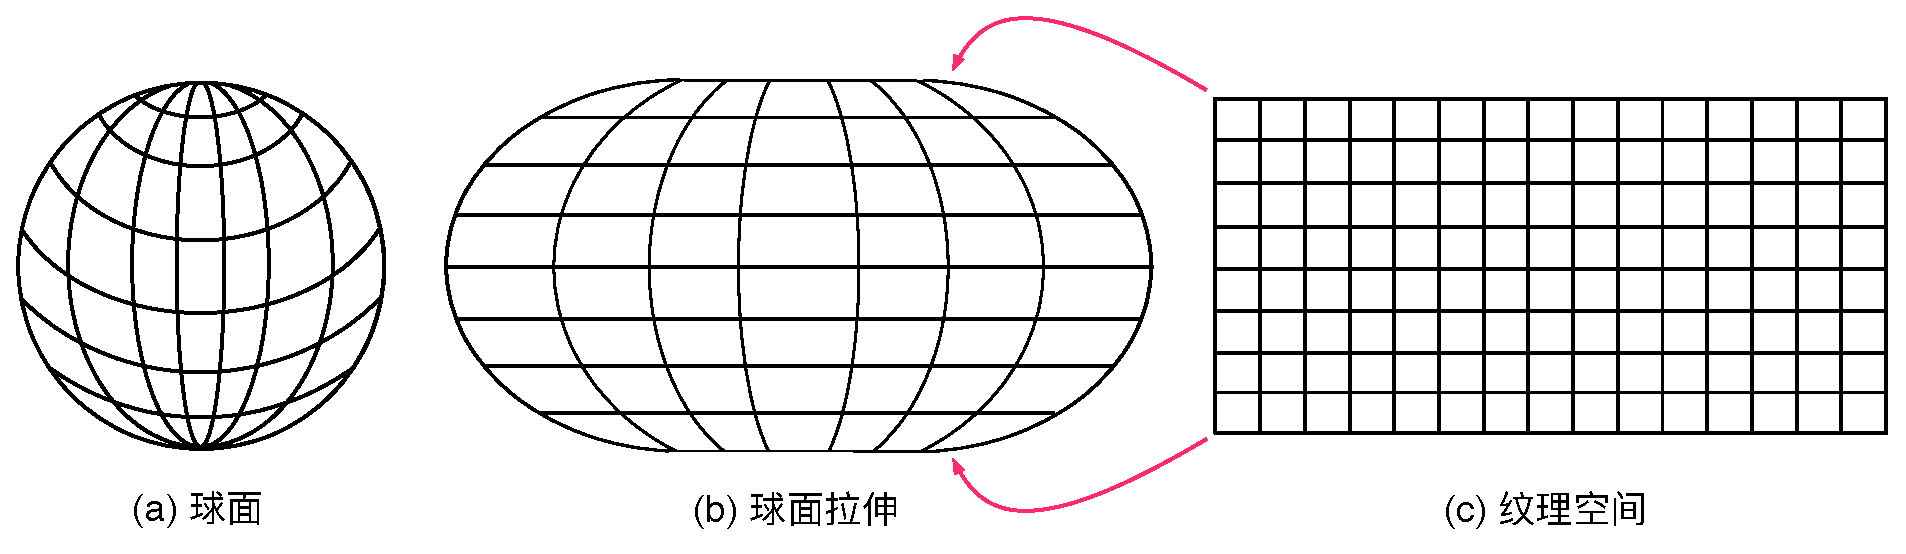
\includegraphics[width=\textwidth]{figures/pl/polar-coordinates}
	\caption{极坐标可以被用于实现对球面向图像平面的映射,这个过程可以看做沿着某个经度将球面划开,然后沿着两边拉伸(b),直至形成一个矩形形状(c),这个过程也类似于地球被展开到一张矩形地图上的位置映射。}
	\label{f:pl-polar-coordinates}
\end{figure}

尽管极坐标映射的形式看起来非常简单,但实际计算效率却非常低,例如它的投影计算涉及到计算成本非常高的反三角函数计算,另外它也不满足前面介绍的均分采样和线性映射,例如从图\ref{f:pl-polar-coordinates}就可以看出,它仅仅是直接从一个形状经过拉伸形成另一个形状,这种变换显然不是线性的,南北极附近相对于赤道被拉伸得更加厉害。



\subsubsection{球面映射}
球面映射(sphere mapping)\myindex{球面映射}{sphere mapping}是第一个被运用于工业中的环境映射方法,它最早在\cite{a:PyramidalParametrics}中被提出,随后在\cite{a:IlluminationandReflectionMaps:SimulatedObjectsinSimulatedandRealEnvironments,a:TextureMappingasaFundamentalDrawingPrimitive}被更全面地讨论,OpenGL和DirectX都集成了对球面映射的支持。

球面映射的概念非常简单,如图\ref{f:pl-sphere-mapping}所示,我们将一个完全光滑的小球放置于环境的中心(如图中大圆圆心处的小黑点),然后通过一个观察平面(如图中左边垂直于$z$轴的平面)以正交投影(orthographic projection)\myindex{正交投影}{orthographic projection}的方式收集来自该球面上各个方向的入射光照(如图中红色箭头线$\mathbf{r}$所示),这些光照表述的就是位于环境中心处的面向观察平面方向(即$z$轴)半球空间内的入射光照,这个过程可以通过光线追踪的方式进行计算,也可以通过从后面介绍的立方体贴图中投影而来。通过面向$z$和$-z$两个方向分别做一次球面映射就可以得到整个球面的入射光照。

球面贴图(sphere map)\myindex{球面贴图}{sphere map}是通过观察平面计算出来的,该观察平面的宽度和高度都等于光滑球面的直径,观察平面通过正交投影发出的观察光线如黑色的箭头线$\mathbf{v}$所示,这些光线在球面上被反射至入射光线$\mathbf{r}$方向上。从图中可以看出,在位于赤道附近,反射光线几乎反向平行于观察光线,在球面的边缘,反射光线则几乎平行于该球面的正切面。

\begin{figure}
	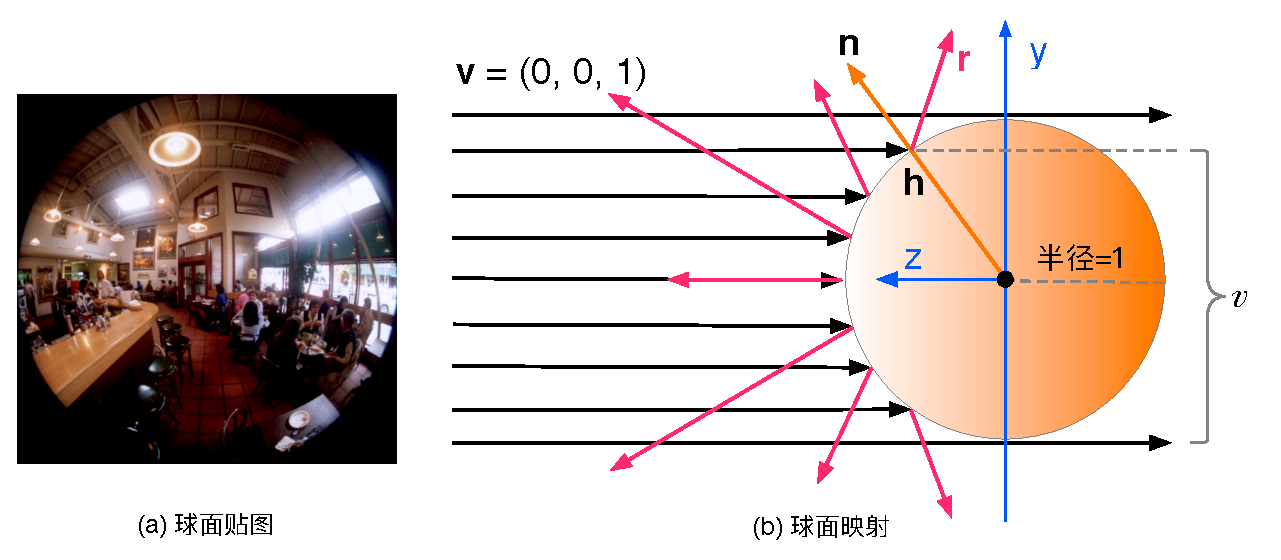
\includegraphics[width=\textwidth]{figures/pl/sphere-mapping}
	\caption{球面映射的概念示意图,一个绝对光滑的球体被放置于环境中心,然后从$z$轴反方向以正交投影的方式向球面发出光线$\mathbf{v}$,该光线经与球面反射后收集来自入射方向$\mathbf{r}$的光照形成球面贴图(左图来自\cite{a:TheStoryofReflectionMapping})。}
	\label{f:pl-sphere-mapping}
\end{figure}

那么,在生成一个球面环境贴图之后,通过给定一个光照的入射方向$\mathbf{r}$,我们怎样得到该贴图上对应的纹理位置呢?换句话说,一个入射方向$\mathbf{r}$是怎样被映射为一个纹理坐标$(u,v)$的?如图\ref{f:pl-sphere-mapping}(b)所示,一个入射方向$\mathbf{r}$到球面贴图的映射,可以看做为观察光线$\mathbf{v}$与球面的交点$\mathbf{h}=(h_x,h_y,h_z)$到球面贴图的映射,而根据正交投影的定义,直接取交点$\mathbf{h}$的$x$和$y$轴的值$(h_x,h_y)$即可作为球面贴图的$(u,v)$值,那么剩下的问题就归结为通过已知的$\mathbf{r}=(r_x,r_y,r_z)$求出其对应的交点$\mathbf{h}$。

由于观察光线$\mathbf{v}$平行于$z$轴,所以其归一化的观察方向可以表述为$\mathbf{v}=(0,0,1)$,因此$\mathbf{v}$与$\mathbf{r}$所对应的法线可以表述为$(r_x,r_y,r_z+1)$,归一化后为:

\begin{equation}\label{e:pl-sm-m}
	\begin{aligned}
		m=&\sqrt{r^{2}_x+r^{2}_y+(r_z+1)^{2}}\\
		\mathbf{n}=&\Bigg(\frac{r_x}{m},\frac{r_y}{m},\frac{r_z+1}{m}\Bigg)
	\end{aligned}
\end{equation}

有了上述法线$\mathbf{n}$的表述,如果假设光滑球面的半径为1,则上述法线$\mathbf{h}$中的分量值正好可以用来表述其对应的交点$\mathbf{h}$的位置。同时由于$(h_x,h_y)$的取值范围为$[-1,1]$,所以我们通过下面的方式将其映射到$[0,1]$:

\begin{equation}
	\begin{aligned}
		u=&\frac{r_x}{2m}+0.5\\
		v=&\frac{r_y}{2m}+0.5
	\end{aligned}
\end{equation}

其中$m$取式\ref{e:pl-sm-m}中的值。

尽管球面映射的整个计算过程相对比较简单,并且整个方向映射没有缝隙,但它依然面临一些缺点。首先球面映射的采样分布是非常不均匀的,例如在靠近$z$轴附近,方向被映射得比较密集,而在靠近球面边缘附近,大量的方向被映射到纹理中圆形区域边缘较窄的面积,这种非线性的特征使得顶点之间的线性插值结果是可能错误的。这非线性可以从图\ref{f:pl-sphere-mapping}(a)中看出,随着入射光线向球面边缘靠近,球面贴图被扭曲越来越严重。

此外,在球面的边缘,由于入射光线$\mathbf{r}$几乎平行于球面的正切面,因此整个球面边缘其实代表一个相同的方向,因此它们具有相同的光照值,又称为一个奇点。在这种情况下,两个顶点之间的插值很有可能是穿过球面背部的部分,但是却可能错误地在球面贴图中的圆形图像内部进行插值\cite{a:Reflectionvectorshadinghardware};此外,在边缘部分,由于较小的表面(像素)面积被映射到更多的方向,因此可能形成比较大的采样方差,是这部分的着色形成一些比较刺眼的斑点或暗点。

最后,由于球面映射只能生成特定观察方向下半个球面的入射光照,另外半个球面的光照则被忽略,因此它是与视角有关的。\cite{a:View-independentenvironmentmaps}在此基础上提出抛物面球面映射,它分别对$z$和$-z$轴分别执行一次球面映射以生产两个覆盖全空间方向的球面贴图,然后这两张纹理被用于环境映射的计算,这里不再详述。



\subsubsection{立方体映射}
\cite{a:EnvironmentMappingandOtherApplicationsofWorldProjections}提出了目前为止工业中最为流行的环境映射算法,该方法称为立方体映射(cube mapping)\myindex{立方体映射}{cube mapping},在该表述中,摄像机被放置于一个环境的中央位置,然后将整个环境分别投影到一个立方体的六个面上。这个投影过程可以很容易地被现代图形处理器实现,例如我们只需要将摄像机分别朝向图\ref{f:pl-cube-mapping}(a)所示的六个方向(即$-x,+x,-y,+y,-z,+z$),然后分别对每个方向执行一次渲染,使每个方向上对应的场景被投影到垂直于该方向的一个2D图像上,如图\ref{f:pl-cube-mapping}(b)所示。在更新的图形处理器接口中,上述过程甚至只需要一个渲染通道就可以完成,我们只需要在几何着色器中修改摄像机的朝向即可。

\begin{figure}
	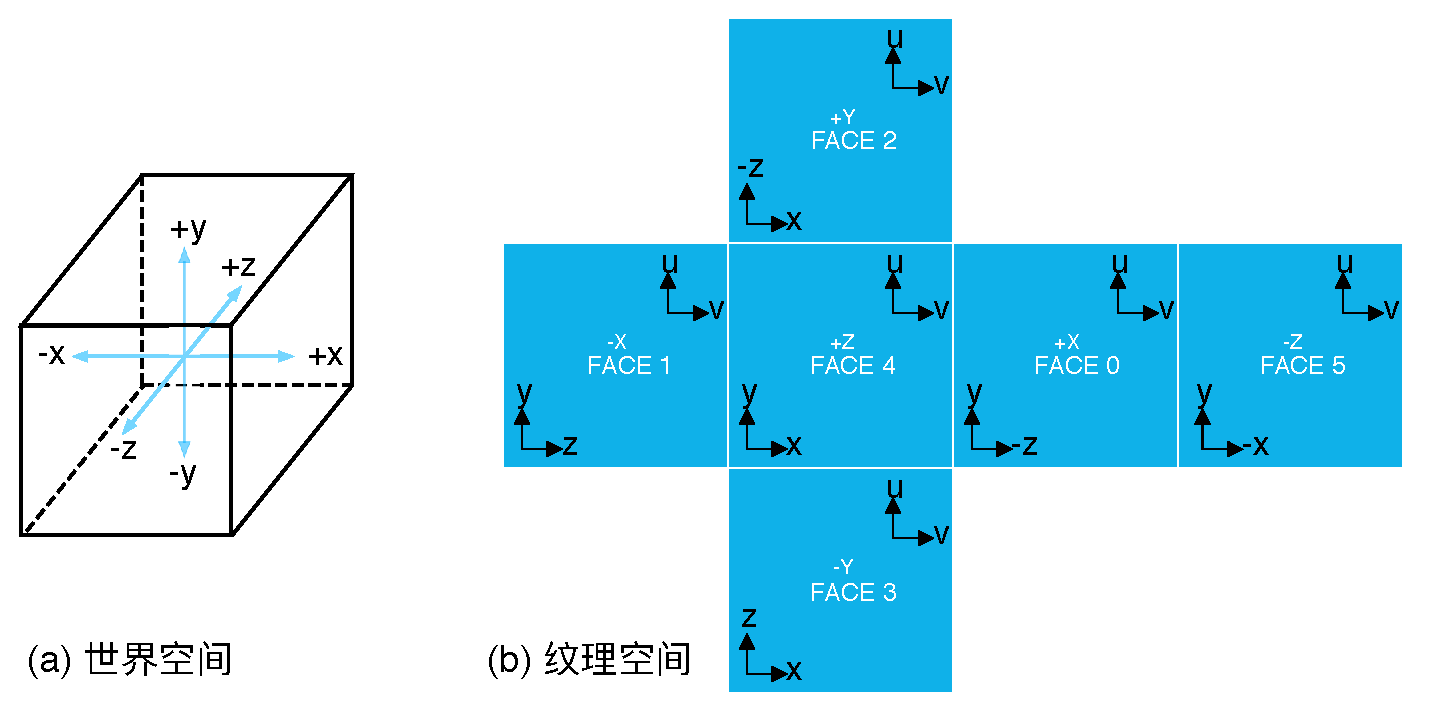
\includegraphics[width=\textwidth]{figures/pl/cube-mapping}
	\caption{立方体映射的过程,它首先将周围环境映射到一个立方体的六个面上(a),然后将该立方体展开即形成一个立方体贴图(b)。}
	\label{f:pl-cube-mapping}
\end{figure}

在立方体映射中,由世界空间的方向向纹理空间的变换非常简单,这只需要将表示方向的范围矢量投影到立方体对应的面即可,该面上对应投影使用的坐标值即可作为立方体贴图中的纹理坐标,例如对于$+y$面上的方向(即图\ref{f:pl-cube-mapping}(a)中立方体的上平面),其对应的纹理坐标为方向矢量在$-zx$平面上的投影(如图\ref{f:pl-cube-mapping}(b)中最上面的FACE2正方形平面)。

立方体映射的主要优点是整个映射是分段线性映射,即在立方体的每个面内的映射是线性的;立方体映射的主要缺点是它的光照值需要分别存储的6个纹理中,例如在读取的时候需要额外区分每个方向对应于立方体的哪一个面,这会导致在着色器中形成分支选择;此外,位于每个面中心位置处的纹素相对于正方形边缘附近的纹理对应于更小的立体角,这使得立方体映射表述的方向密度是不均匀的;最后,所有方向被存储在不同的纹理中,这使得跨越多个面的顶点之间的插值计算变得比较困难。



\subsubsection{八面体映射}
通过对前面这些环境映射技术的比较,我们可以推导出一种比较理想的环境映射方法,它既应该拥有球面映射那样的将整个球面的所有方向表述在一张纹理上的能力,又应该具有立方体映射那样具有线性映射和高效索引的特征,八面体映射就是一种比较接近这种要求的环境映射方法。

\begin{figure}
	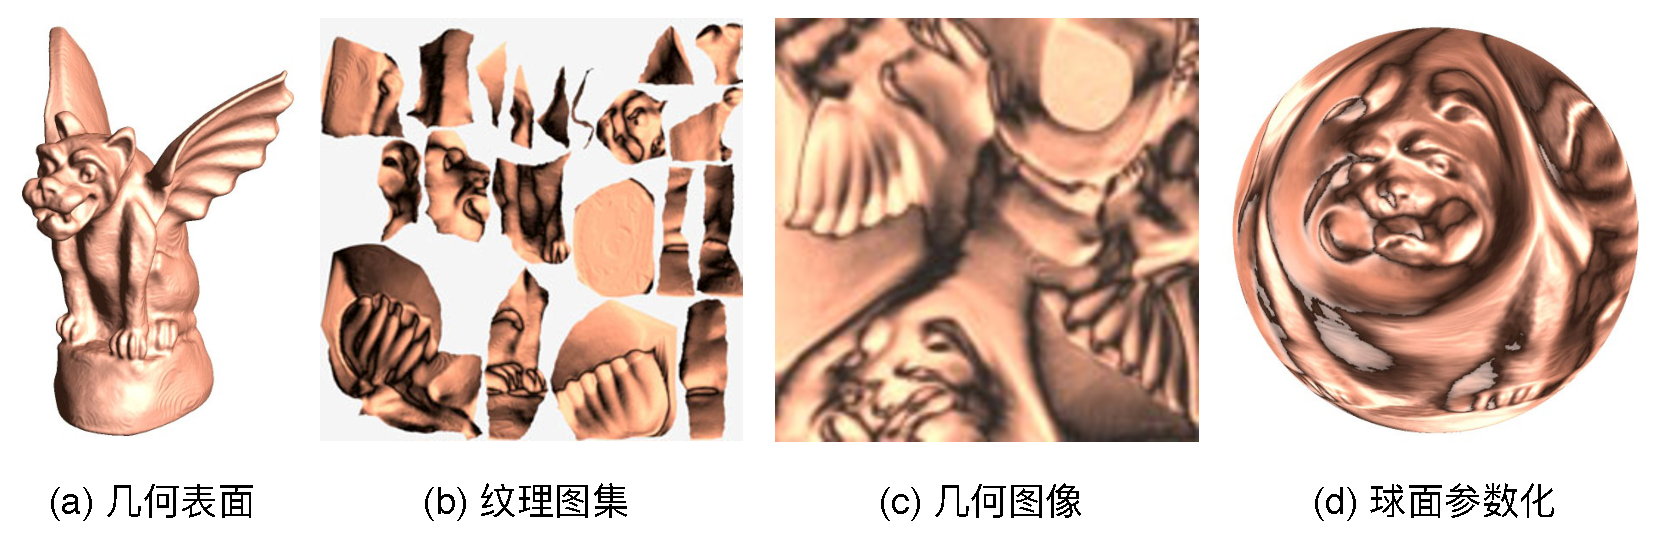
\includegraphics[width=\textwidth]{figures/pl/surface-parametrization}
	\caption{几种不同的表面参数化表述及其演进(图片来自\cite{a:SphericalParametrizationandRemeshing})。}
	\label{f:pl-surface-parametrization}
\end{figure}

八面体映射(octahedron mapping)在计算机图形学中的运用最早要追溯到对表面参数化的改进,表面参数化(surface parametrization)\myindex{表面参数化}{surface parametrization}是指将几何物体的表面与一个平面域(planar domain)\myindex{平面域}{planar domain}建立一种联系,使得我们可以对表面提供各种需要的属性,这即是对表面建立一种参数表述。传统的做法是将表面划分成多个图块(charts)\myindex{图块}{charts},然后让它们分别与平面域上的某个区域建立一种映射,这些平面域上对应的区域即是对该表面图块的参数化,这个平面域上的区域的集合称为一个纹理图集(texture atlas)\myindex{纹理图集}{texture atlas}\cite{a:Texturemappingprogressivemeshes,a:Interactivetexturemapping,a:Ageneralmethodforpreservingattributevaluesonsimplifiedmeshes,a:Leastsquaresconformalmapsforautomatictextureatlasgeneration},如图\ref{f:pl-surface-parametrization}(b)所示,这也即是当前工业中对物体网格表面进行参数化的主要形式,这些纹理图集可以用来存储各种表面属性数据,如法线,漫反射系数等。

然而纹理图集的缺点是各个图集之间有不连续的缝隙,如图\ref{f:pl-surface-parametrization}(b)所示,这种缝隙不仅会反应在着色的表面上,而且会使得对纹理的过滤操作产生错误的结果。为了弥补这种缺陷,\cite{a:Geometryimages}提出一种称为几何图像(geometry images)\myindex{几何图像}{geometry images}的概念,该方法将整个几何表面映射为一个完整的2D图像,该几何图像因此不包含任何缝隙,如图\ref{f:pl-surface-parametrization}(c)所示。

基于几何图像的思路,\cite{a:SphericalParametrizationandRemeshing}进一步提出了球面参数化(spherical parametrization)\myindex{球面参数化}{spherical parametrization}的方法,该方法认为,对于一个零亏格\footnote{在数学上,亏格(genus)是指一个自闭的表面包含的“洞”的数量,参见\url{https://en.wikipedia.org/wiki/Genus_(mathematics)}}(genus-zero)\mathindex{零亏格}{genus-zero}的几何表面,假如它们的表面细节变化不是特别复杂(例如那些由球面简单变形而来的表面),则这些表面完全可以使用一个球面域(spherical domain)\myindex{球面域}{spherical domain}来进行参数化,即我们可以将整个表面区域“展开”到一个球面作用域上,使表面上的每个区域对应于该球面域上的某个部分,即表面与球面域之间形成1对1的映射。例如在图\ref{f:pl-spherical-parametrization}中,一个零亏格的闭合曲面被首先映射到一个球面域,然后这个球面域被映射到一个正方面体上,最后这个正八面体被展开为一个参数化的2D纹理。
	
\begin{figure}
	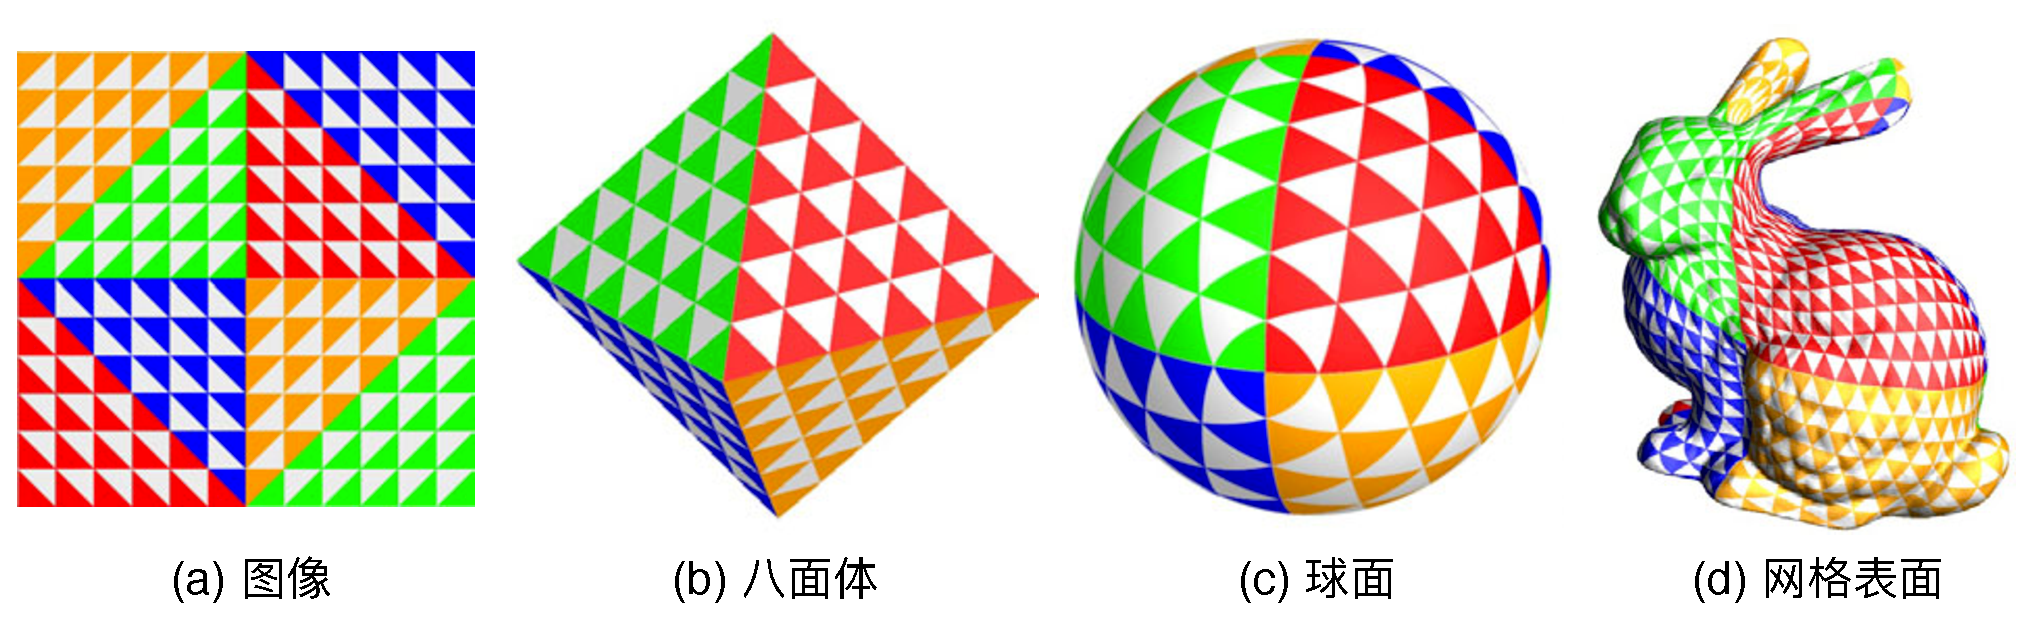
\includegraphics[width=\textwidth]{figures/pl/spherical-parametrization}
	\caption{球面参数化的基本概念,从右到左,首先一个零亏格的闭合曲面(d)被映射到一个球面域(c)上,然后球面投影到一个八面体上(b),最后八面体展开为一个2D图像(a),这样整个曲面被参数化为一个无缝的2D纹理(图片来自\cite{a:SphericalParametrizationandRemeshing})。}
	\label{f:pl-spherical-parametrization}
\end{figure}

虽然球面参数化方法的提出是用于解决表面表述的问题,但是对于环境映射的问题,如果将整个周围环境中的表面看做一个零亏格的单个几何物体,那么我们可以使用球面参数化的思路将这个“环境几何表面”参数化到一个球面域,这个球面域上的每个点对应于一个入射方向的光照值,整个环境被均匀地映射到一个球面域上,这就是\cite{a:OctahedronEnvironmentMaps}提出的八面体环境贴图(octahedron environment maps)\myindex{八面体环境贴图}{octahedron environment maps}的基本思路。

球面参数化和环境映射的区别是,球面参数化需要去构造一个均匀的方向分布,来使曲面被更好地映射到一个球面域上,进而被参数化为一个2D纹理,也就是图\ref{f:pl-spherical-parametrization}中由(d)到(c)的一步;然而对于环境映射,这个球面域其实是已知的,我们只需要对每个方向存储一个光照值即可,即它只包含图\ref{f:pl-spherical-parametrization}中的(a)(b)和(c)两个步骤,也就是怎样将一个球面域投影到一个正八面体上,以及怎样将一个正八面体展开为一个2D图片。



\paragraph{球面域向八面体面的投影}
几何中的八面体是指拥有八个面,12条边和6个顶点的多面体,我们常使用的八面体通常是指由八个等边三角形构成的正八面体,其中每4个面共享一个顶点,如图\ref{f:pl-octahedron-mapping}左图所示,以下我们所讨论的八面体都是指这种正八面体。

前面介绍的几种环境映射方法都是直接将球面域映射到2D的纹理空间,而八面体映射需要首先将球面域映射到一个中间的八面体结构,然后再由八面体展开形成2D的图像,表面上看起来这更复杂了,然而以下我们将看到八面体有一种特殊的性质使得这个映射算法反而更加简单高效。

\begin{figure}
	\sidecaption
	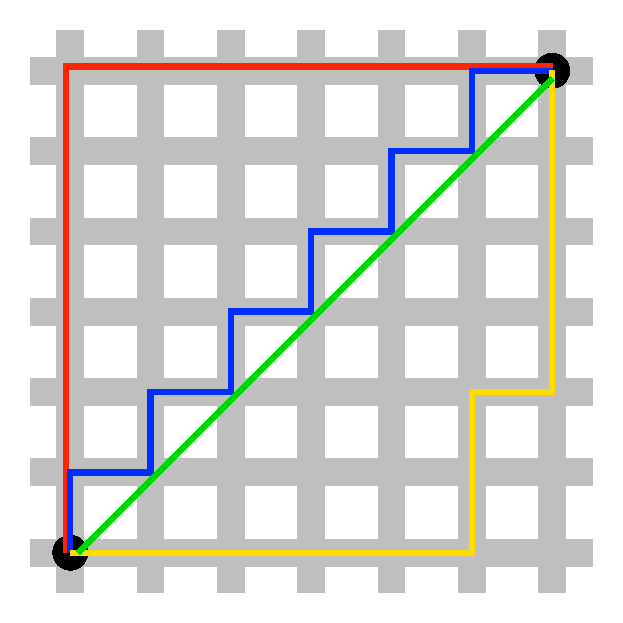
\includegraphics[width=0.4\textwidth]{figures/pl/manhattan-distance}
	\caption{出租车几何学中的曼哈顿距离与传统欧几里得距离的比较,在出租车几何学中,红,黄和蓝三条路径具有相同的最短距离12,在欧几里得几何中则只有绿色一条最短路径为$6\sqrt{2}\approx 8.49$(图片来自Wikipedia,作者:Psychonaut)。}
	\label{f:pl-manhattan-distance}
\end{figure}

一般的映射算法都涉及到一些高次的乘/除法或者三角函数计算,例如式\ref{e:pl-sm-m}中的归一化系数就涉及乘法和开方的计算,然而正八面体却具有一种特殊的属性使得其仅使用最简单的加法运算就可以实现由球面域到正八面体的映射。在出租车几何学(taxicab geometry)\mathindex{出租车几何学}{taxicab geometry}中,我们使用另一个不同于笛卡尔坐标系下的距离度量(如$|d|=\sqrt{x^{2}+y^{2}+z^{2}}$),那就是两点之间的距离等于每个对应分量的绝对差值的和,例如$ds=dx+dy+dz$,这个距离度量又称为直角距离(rectilinear distance)\mathindex{直角距离}{rectilinear distance},$L^{1}$范数($L^{1}$ norm)或者曼哈顿距离(Manhattan distance)\mathindex{曼哈顿距离}{Manhattan distance}等,它指示了一辆出租车在两个位置之间行驶的最短距离,如图\ref{f:pl-manhattan-distance}所示。

对于一个正八面体,假设其两个顶点的坐标分为为$(\pm r,0,0),(0,\pm r,0)$和$(0,0,\pm r)$,其中$r$为正八面体的中心距离任意一个顶点的距离,由正八面体的几何特征可得,任意一个点$p=(p_x,p_y,p_z)$位于正八面体的面上的条件是$p$到正八面体中心点的曼哈顿距离为$r$,即$|p_x|+|p_y|+|p_z|=r$。根据上述性质,对于一个位于由正八面体的顶点构成的球面上的点$p$,我们可以通过下述方式得到它在八面体上的投影$p^{'}$:

\begin{equation}\label{e:pl-octahedron-projection}
	p^{'}=\frac{p}{|p_x|+|p_y|+|p_z|}
\end{equation}

上述的投影操作仅涉及到最简单的加法运算,计算效率非常高;同时由于上式只是对$p$点位置各个分量的等比缩放,因此投影到正八面体上的的点$p^{'}$仍位于由$p$到原点构成的直线上,如图\ref{f:pl-octahedron-mapping}右图所示。

\begin{figure}
\begin{fullwidth}
	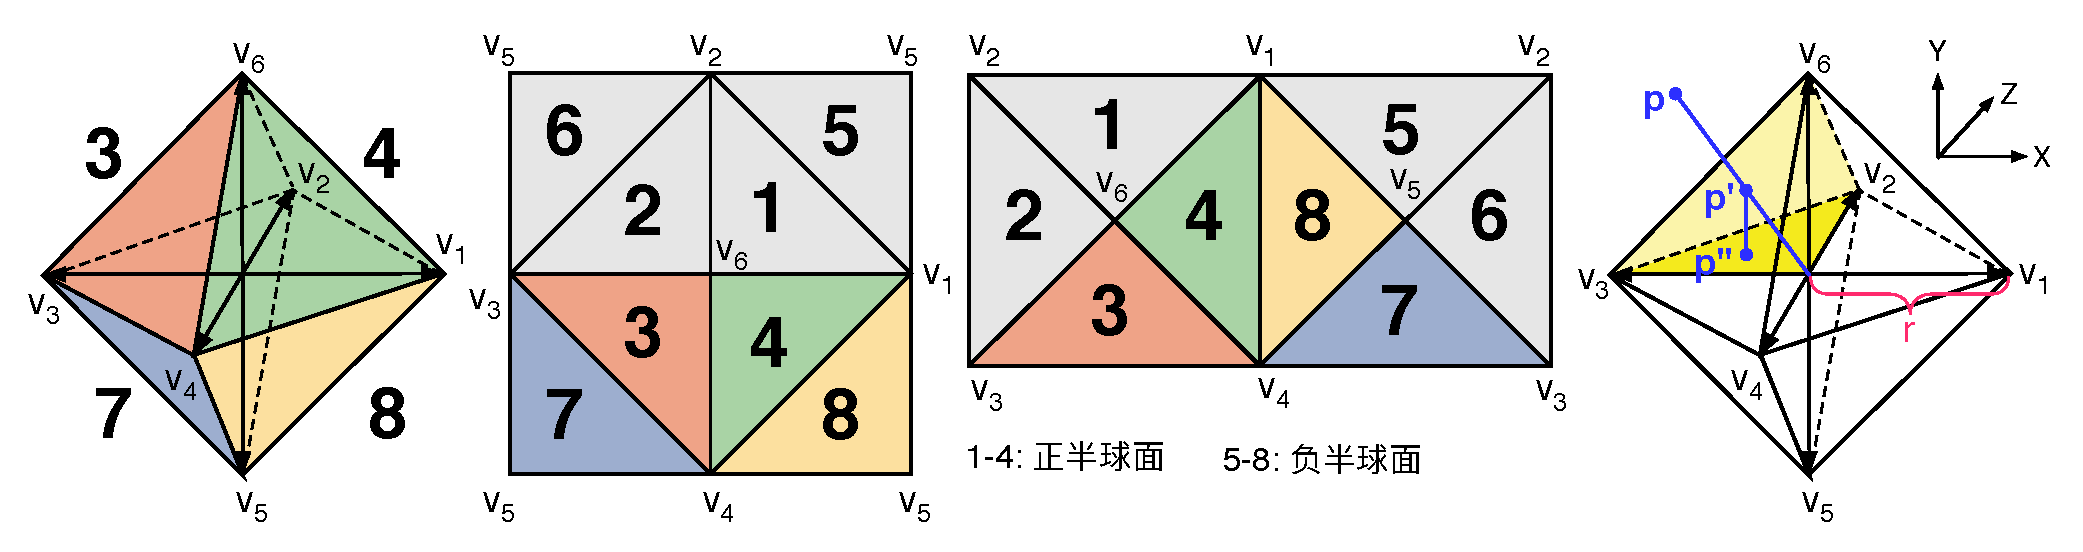
\includegraphics[width=\thewidth]{figures/pl/octahedron-mapping}
	\caption{八面体映射的基本概念,球面上代表方向的点首先被投影到八面体的面上,然后八面体被展开为一个正方形或者矩形的2D图像(图片来自\cite{a:OctahedronEnvironmentMaps})。}
	\label{f:pl-octahedron-mapping}
\end{fullwidth}
\end{figure}



\paragraph{八面体面的展开}
为了将正八面体展开为一个正方形,对于所有位于正半球面上的点,即$p_y>0$,我们将它直接正交投影到XZ平面(即是仅取X和Z轴上的分量),这形成四个全等的等腰直角三角形,其要长均为$r$,如图\ref{f:pl-octahedron-mapping}左二图中的1,2,3和4面,并且这四个等腰直角三角形构成一个正方形;对于负半球面上的点,我们首先仍然按类似的方式投影到ZX平面形成四个等腰直角三角形,然后将这些等腰三角形沿其与上面的三角形的交线向外展开,形成图\ref{f:pl-octahedron-mapping}左二图中的5,6,7和8面。上述的过程可以按下式进行计算:

\begin{equation}
	p^{''}_q=\begin{cases}
		(p^{'}_x,0,p^{'}_z)  & p^{y}\geq 0\\
		(\sigma(p^{'}_x)(1-\sigma(p^{'}_z))p^{'}_z,0,(\sigma(p^{'}_z)(1-\sigma(p^{'}_x))p^{'}_x) & p^{'}_y<0
	\end{cases}
\end{equation}

这里$\sigma(x)$是一个符号函数。

除了上述的方法,我们还可以将正八面体投影到一个比率为$2:1$的矩形纹理上,首先同样是将所有面正交投影到ZX平面上形成8个等腰直角三角形,然后我们将其中一对上下相邻面沿其公交线展开,最后在分别将上下半球的面沿八面体的上下顶点展开,如图\ref{f:pl-octahedron-mapping}右二图所示,该过程可以按下式进行计算:

\begin{equation}
	p^{''}_r=\begin{cases}
		(p^{'}_x-p^{'}_z-1,0,p^{'}_x+p^{'}_z) & p^{'}_y\geq 0 \\
		(p^{'}_z-p^{'}_x+1,0,p^{'}_x+p^{'}_z) & p^{'}_y< 0
	\end{cases}
\end{equation}

根据图\ref{f:pl-octahedron-mapping}的布局可知,$p^{''}_r\in[-2,2]\times [-1,1]$,而$p^{''}_q\in [-1,-1]^{2}$。

八面体环境映射是一种计算效率非常高的映射方法,这得益于它将$L^{2}$范数转换为$L^{1}$范数,它的映射仅仅涉及到加法的运算,同时每个面内方向的映射也是线性的,它的方向分布也非常均匀,\cite{a:ASurveyofEfficientRepresentationsforIndependentUnitVectors}对通过几种环境映射算法进行比较,八面体映射也是误差非常低的一种映射方法。




\subsection{预过滤}\label{sec:pl-pre-filtering}
对于一个给定位置处的入射光照场$L(l)$,例如本节介绍的环境贴图,给定观察方向$v$上的出射辐射亮度 $R(v)$可由下述反射方程计算得出:

\begin{equation}\label{e:pl-prefiltering-1}
	R(v)=\int_H L(l)f(l,v)(n\cdot l){\rm d}l
\end{equation}

上式意味着,对于表面上的每一个位置,我们都需要计算围绕该点法线方向上整个半空间范围$H$内的一个积分,该积分的被积函数为入射光照场与反射分布函数以及几何项的乘积。对于绝对光滑的镜面表面,其反射分布函数只包含一个唯一的入射方向,此时上述的积分退化为单个函数值的计算,如果入射光照场存储为一个环境贴图,则这意味着每个像素位置只需要一次纹理查询操作,正如本节前面介绍的那要,如图\ref{f:pl-pl-pre-filtering-3}和\ref{f:pl-pl-pre-filtering-1}(a) 所示;然而对于光泽反射,由于表面具有一定的粗糙度,因此同一观察方向可以接受来自多个入射方 向的光照,如图\ref{f:pl-pl-pre-filtering-1}(b)所示,此时每个表面像素的着色都需要执行一个积分计算,这种计算成本对于实时渲染来说是不可承受的,本节我们就来讨论怎样 计算使用环境贴图光照下的光泽和漫反射。

\begin{figure}
	\sidecaption
	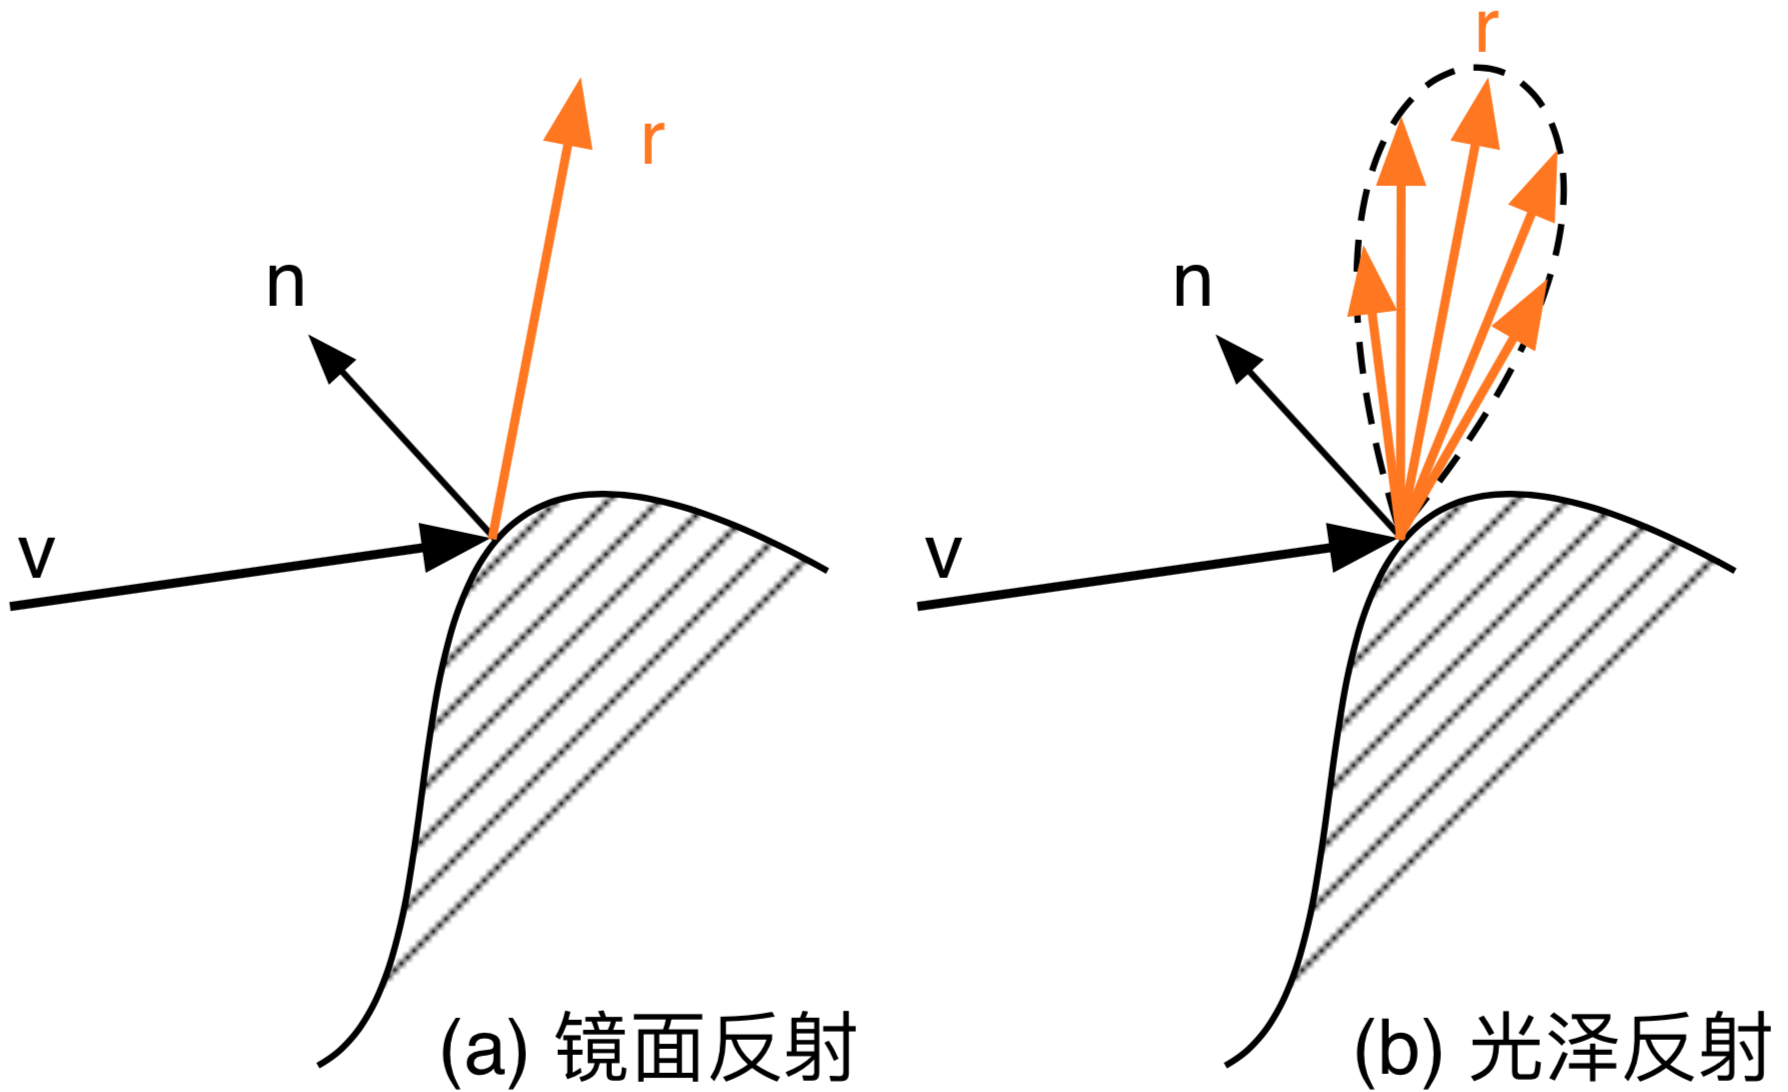
\includegraphics[width=0.65\textwidth]{figures/pl/pl-pre-filtering-1}
	\caption{对于环境贴图表述的入射光照场,镜面表面反射只需要执行一次纹理查询操作(a),而光泽表面具有一定的粗糙度,因此它需要执行多次纹理查询操作(b),每个查询方向的光照被反射分布函数加权后形成对入射光照的贡献}
	\label{f:pl-pl-pre-filtering-1}
\end{figure}

对于式\ref{e:pl-prefiltering-1},$L(l)$可以被看做一个未过滤的原始环境贴图,如果将BRDF函数看做一个用于加权各个方向入射辐射亮度的核函数,则可以将这个对入射辐射亮度的加权计算预先计算并存储起来,形成一个预过滤的环境贴图,该预过滤的环境贴图存储的是每个观察方向$v$上的辐射亮度,它通过对入射辐射亮度场$L(l)$使用BRDF函数执行加权计算而出,这样在实时渲染着色的时候只需要对该预过滤环境贴图执行一次查询操作(就像原始环境贴图对于镜面反射那样)即可,我们称这样的预计算操作为预过滤(prefiltering)\myindex{预过滤}{prefiltering},并称这种预过滤后的环境贴图为反射贴图(reflection map)\myindex{反射贴图}{reflection map},预过滤的目的是将加权的积分计算过程放到预处理阶段,以加速实时计算的性能,它使得实时计算的成本被 降低到一个固定开支,例如单次纹理查询的成本。

从上述的分析来看,预过滤计算本身是很简单的,它仅仅是将一个积分计算预先计算出来而已,其中的过滤器可以具有任意的形式,例如不同的窗宽,各向异性等属性。然而本节的难点在于,我们希望把这种预过滤结果存储在纹理中以供着色器执行像素查询操作,由于表面上每个位置处的BRDF函数可能具有不同的形式(例如不同的窗宽),这就给反射贴图增加了维度以及复杂度,本节后面的主要内容就是讨论这些不同BRDF形式下的预过滤技术。

此外,除了运用于环境贴图光照的预计算,预过滤技术也是实时渲染中常用而高效的一种技术手段,我们还将在后面的章节继续介绍它的其它运用。




\subsubsection{漫反射表面}
首先来看最简单的漫反射模型,对于漫反射,其BRDF函数对于所有观察和入射方向是一个常数,即$f_{\rm diff} = c_{\rm diff}/\pi$,其中$c_{\rm diff}$为漫反射表面的漫反射率,将该BRDF常数代入式\ref{e:pl-prefiltering-1},则该式转换为漫反射率 $c_{\rm diff}$ 与以下辐射照度的乘积:

\begin{equation}\label{e:pl-prefiltering-2}
	\int_H \cfrac{L(l)(n\cdot l)}{\pi}{\rm d}l
\end{equation}

上式表述的是一个特定的法线方向对应的辐射照度,由于它只与方向有关,因此同样可以使用前面的环境贴图的表述形式进行存储,例如立方体贴图,不同的是,这里每个值存储的是一个辐射照度(irradiance)值,因此这种预过滤的环境贴图又称为辐射照度环境贴图(irradiance environment maps)\myindex{辐射照度环境贴图}{irradiance environment maps}\cite{a:IlluminationandReflectionMaps:SimulatedObjectsinSimulatedandRealEnvironments},该贴图通过一个法线方向进行索引(或者说辐射照度是关于法线的函数),如图\ref{f:pl-f:pl-pl-pre-filtering-2}(a)所示。

\begin{figure}
	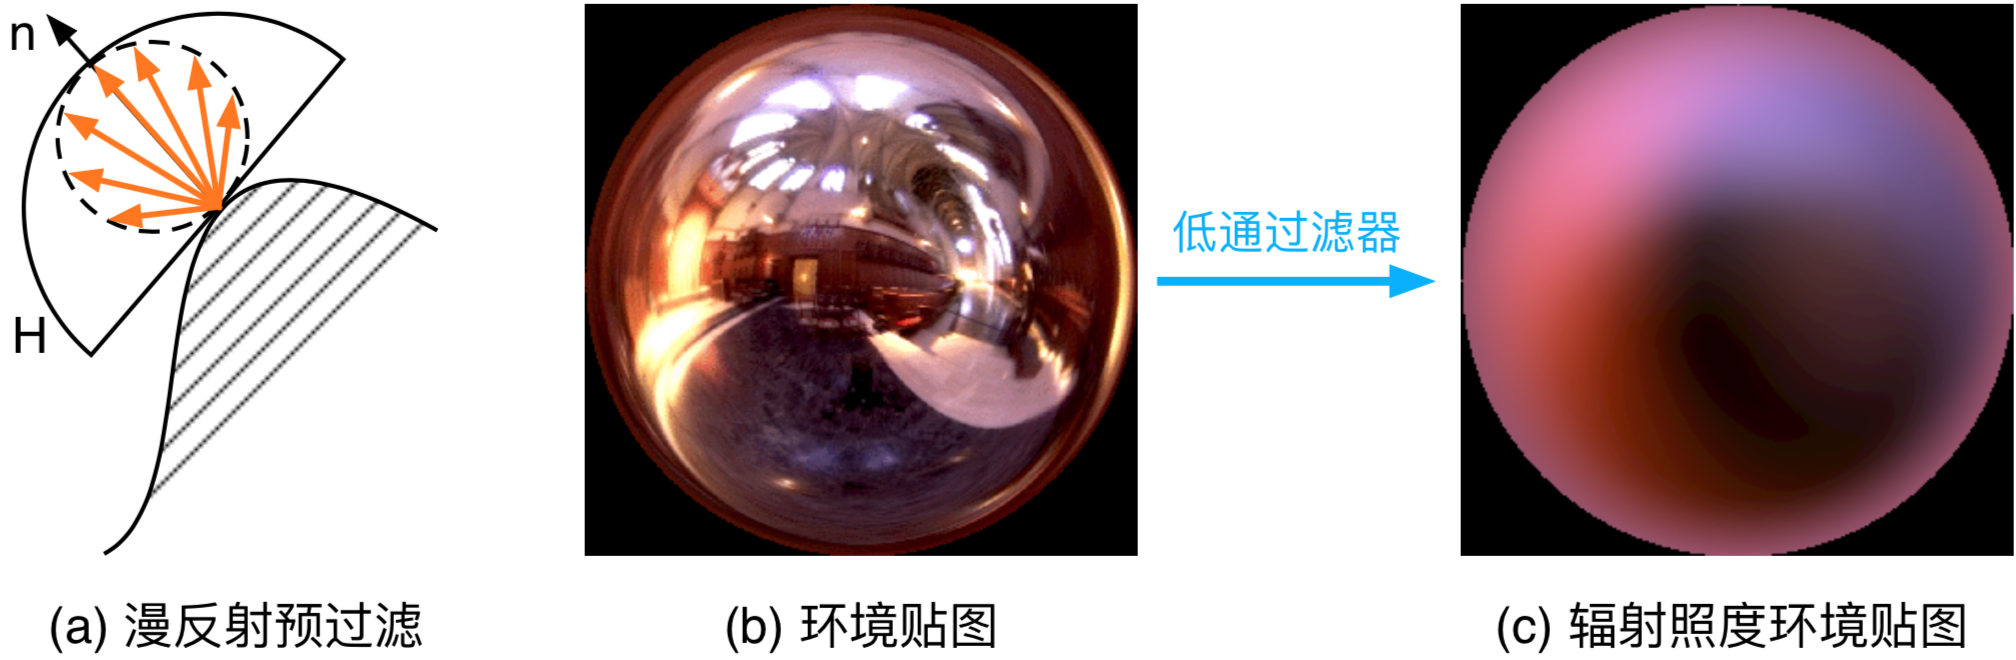
\includegraphics[width=\textwidth]{figures/pl/pl-prefiltering-2}
	\caption{漫反射表面的预过滤计算,其过滤函数为法线方向面对的半空间$H$内法线和入射方向夹角的余弦函数,其预过滤计算的值又称为辐射照度,它被存储在一个辐射照度贴图中(c),通过法线方向索引查询(图片来自于\cite{a:Anefficientrepresentationforirradianceenvironmentmaps})}
	\label{f:pl-f:pl-pl-pre-filtering-2}
\end{figure}

由于漫反射光照可以看做是对原始高频的环境贴图作用了一个低通过滤器(low pass filter)\myindex{低通过滤器}{low pass filter},如图\cite{f:pl-f:pl-pl-pre-filtering-2}(b)和(c)所示,因此辐射照度的频率变化非常低,它可以使用非常低分辨率的贴图进行存储,也可以使用前面介绍的球谐函数进行表述 \cite{a:Anefficientrepresentationforirradianceenvironmentmaps}。



\subsubsection{光泽表面}
从上一节的内容可以看出,漫反射光照的预过滤使用的是一个空间不变的(space invariant)\myindex{空间不变的}{space invariant}过滤器(即余弦函数),因此对原始环境贴图上的每一个像素使用一个相同的过滤器。然而光泽表面的BRDF函数则要复杂得多,光泽表面的BRDF函数通常是空变的(space variant)\myindex{空变的}{space variant}或者说移变的(shift variant)\myindex{移变的}{shift variant},即表面上不同位置处使用完全不同的BRDF核函数,这可能是由于粗糙度变化引起的,例如不同粗糙度对应的BRDF函数具有不同的窗宽,也可能是由于各向异性造成的,例如不同反射方向的BRDF函数具有不同的形式。

要讨论任意BRDF作为核函数的预过滤是非常复杂的,当前也没有比较统一且高效的方法能够处理任意BRDF函数的预过滤,后面的内容我们将聚焦于各向同性的(isotropic)BRDF分布函数,这也是目前工业中比较主流的方案,读者应能够通过了解光泽表面预过滤技术的基本原理及思路,去阅读和理解更一般的BRDF函数下的预过滤。

本节将首先讨论最简单的冯氏BRDF模型,冯氏模型之所以简单,是因为它不仅是各向同性的,并且它的反射函数形状仅与粗糙度有关,而与反射方向和表面的法线无关,这使得在同一粗糙度下,冯氏模型的核函数是固定的,也就是我们可以近似地用粗糙度来表述冯氏BRDF函数的窗宽。

冯氏BRDF模型(Phong model)\myindex{冯氏模型}{Phong model}可以表述为:

\begin{equation}
	f_{\rm phong}(v,l)=k_s\cfrac{(r\cdot l)^{N}}{n\cdot l}
\end{equation}

\noindent 其中,$k_s$和$N$分别表述的是冯氏BRDF函数的形状和尺寸,将上式代入式\ref{e:pl-prefiltering-1}得到:

\begin{equation}
	\begin{aligned}
		L_{\rm phong}(r)=&\int_H k_s\cfrac{(r\cdot l)^{N}}{n\cdot l}L(l)(n\cdot l){\rm d}l\\
		=&k_s\int_H(r\cdot l)^{N}L(l){\rm d}l
	\end{aligned}
\end{equation}

由上式可以看出,对于同一粗糙度$N$,冯氏BRDF作为预过滤的核函数$(r\cdot l)^{N}$是相同的(注意这里表面的反射系数$k_s$被提到积分外面,并不参与预过滤计算),这和上一节中介绍的漫反射的情形是类似的;此外,由于冯氏模型只与反射方向有关,因此这里使用反射方向来索引预过滤的环境贴图,这里预过滤的环境贴图中存储的是辐射照度值,即前面介绍的反射贴图,在着色的时 候这个值从贴图中查询并与反射系数$k_s$相乘后作为表面像素的出射辐射亮度, 这种方法最早在\cite{a:Realistichardware-acceleratedshadingandlighting,a:IlluminationandReflectionMaps:SimulatedObjectsinSimulatedandRealEnvironments}被提出。

除此之外,我们还需要考虑对不同粗糙度表面的预过滤,这需要分别对每个粗糙度系数$N$ 做一个单独的预过滤以生成一个不同的反射贴图,这样将会面临比较大的存储压力。实践中,这些指数形式的粗糙度往往被转换为多级纹理的形式\cite{a:Efficientreflectanceandvisibilityapproximationsforenvironmentmaprendering,a:Efficientrenderingofspatialbidirectionalreflectancedistributionfunctions},即以渐进的方式生成一系列 反射贴图(预过滤的环境贴图),它们一起被存储进一个多级纹理(mip map) 当中(例如多级立方体贴图),其中多级纹理的每一级使用相对前一级具有2倍 标准差的高斯函数,例如$\sigma_{j+1} = 2\sigma_j$ 。最后,在实时着色计算的时候,首先根据表面的粗糙度计算出多级纹理的层级,然后使用双线性插值计算出实际的纹理值。

冯氏模型是最简单的光泽BRDF模型,因为它的微表面法线分布就是一个高斯函数,其中粗糙度由高斯函数的标准差控制,其反射函数的形状与观察方向和法线的夹角无关。另一些更一般的各向同性BRDF模型是与观察方向

和法线的夹角有关的,所谓BRDF函数是各向同性的(isotropic),通常是指BRDF函数的形状围绕法线是成圆对称的,这意味着还需要一个额外的维度用以存储观察方向与法线的夹角,\cite{a:Approximationofglossyreflectionwithprefilteredenvironmentmaps,a:Reflectionspaceimagebasedrendering}对一般的各向同性BRDF做了一些近似处理,在这些近似假设下,原始的高维辐射照度函数被降维,使得仍然可以像冯氏模型那样仅用一个反射方向就可以查询反射贴图的值,这里不再详述,我们会在后面介绍一个快速计算一般各向同性BRDF模型的预过滤方法。



\subsubsection{阶层式预过滤}
前面的两节介绍了环境贴图预过滤使用的两种不同的过滤器,它们分别对应两种不同的BRDF模型,即漫反射BRDF和冯氏BRDF模型。本节我们将聚焦于,给定一个过滤器,怎样高效地执行预过滤计算本身,因此本节的内容与具体过滤器的形式无关。传统的预过滤计算使用的是一种暴力(brute force)方法,即对于每个像素的过滤,它使用周围的每个像素与过滤器中对应的每个离散值进行加权计算,这种计算方法虽然精确,但是计算成本也非常高,特别是如果我们希望这个预过滤计算实时发生,本节我们将介绍一种高效且通用的阶层式预过滤计算框架。

首先回顾一下预过滤的过程,如图\ref{f:pl-pl-pre-filtering-3}所示,为了要计算反射贴图中的一个像素值,如图\ref{f:pl-pl-pre-filtering-3}(a) 中的小黑点所示,我们将一个给定的过滤器作用与原始环境贴图上相同的位置,然后用该核函数与该核函数覆盖的原始环境贴图区域执行卷积计算,该卷积计算的结果及时预过滤的结果。

\begin{figure}
	\sidecaption
	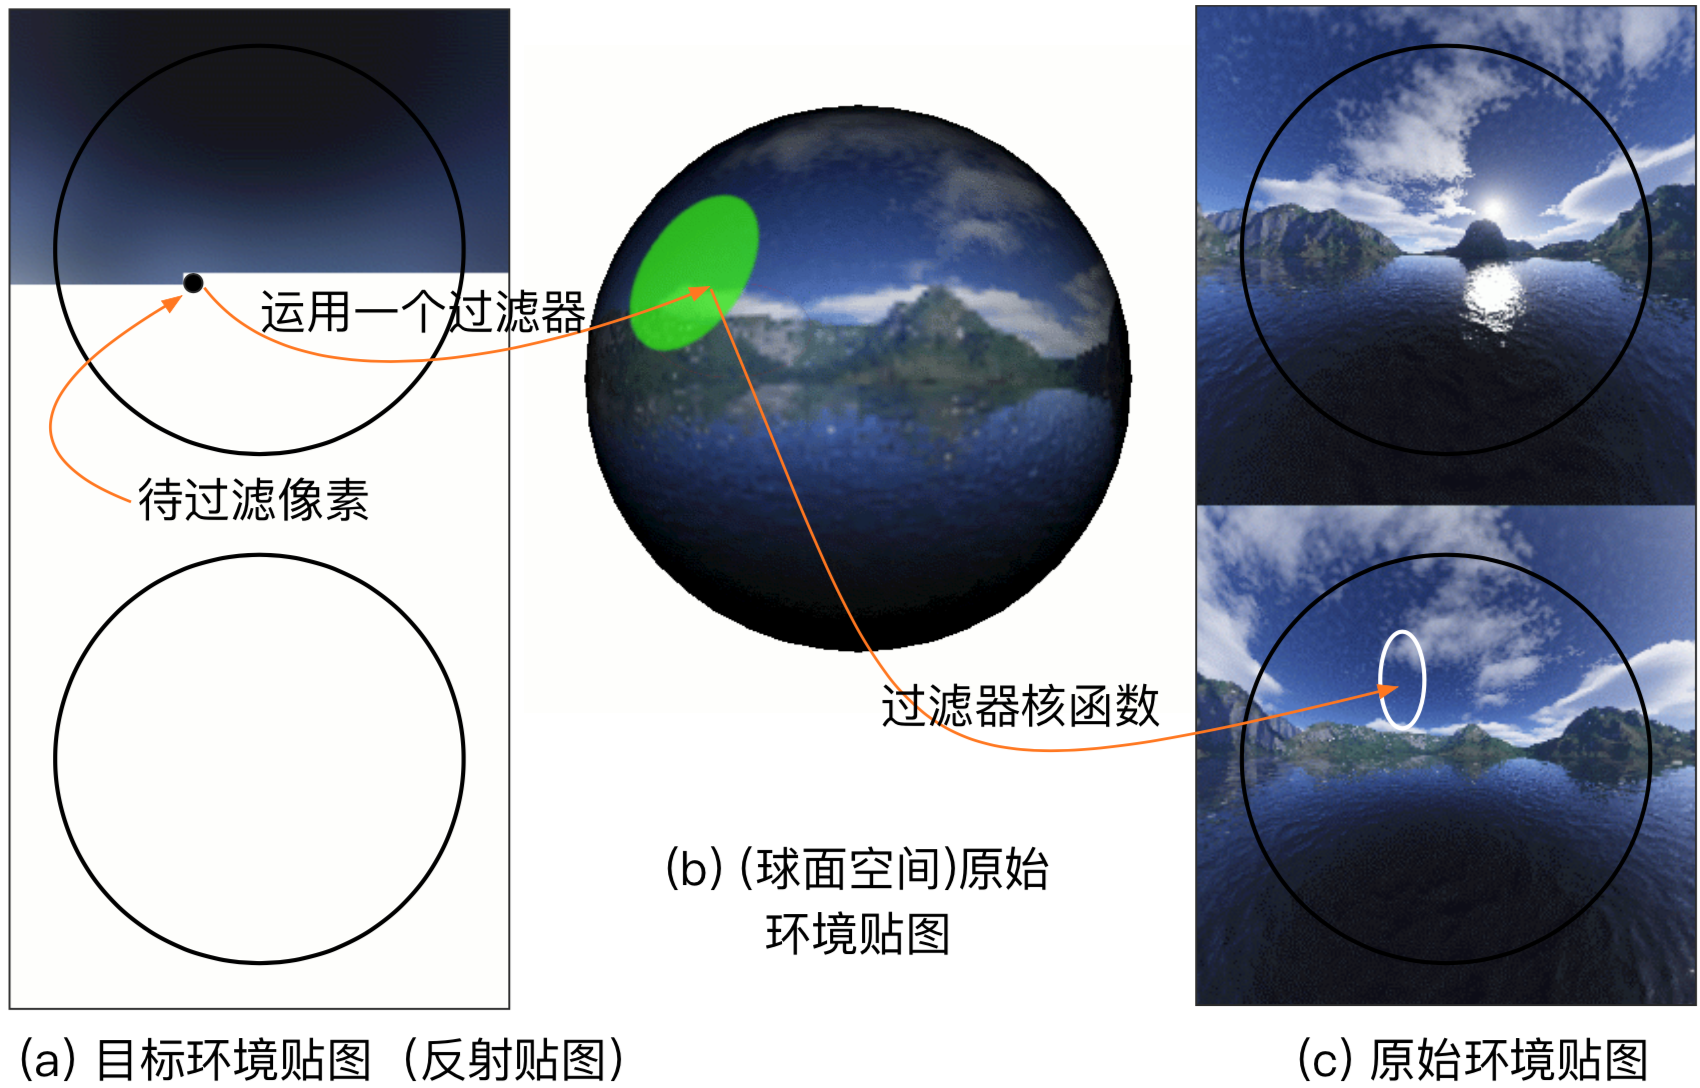
\includegraphics[width=0.65\textwidth]{figures/pl/pl-prefiltering-3}
	\caption{预过滤的过程:对于目标反射贴图(a),它的每一个像素值来自于将一个过滤器核函数 (绿色圆形区域)作用于原始环境贴图中该像素的位置处(b),其结果为该核函数覆盖区域内像素值的加权平均(图片来自\cite{a:Aunifiedapproachtoprefilteredenvironmentmaps})}
	\label{f:pl-pl-pre-filtering-3}
\end{figure}

由此可知,对于每一个目标贴图中的像素,过滤器中的每一个离散值与原 始环境贴图中对应位置处的像素值相乘,然后对所有这些乘积值相加得到过滤后的值,这使得预过滤计算的过程非常慢。在这个过滤过程中,如果过滤器核函数中的某些区域非常平滑,即频率变化很低,那么我们可以使用对该过滤器核函数进行缩减采样(downsampling)后的版本进行过滤计算,基于此观察,\cite{a:Aunifiedapproachtoprefilteredenvironmentmaps}提出了阶层式预过滤(hierarchical prefiltering)技术。

大部分BRDF分布函数仅在很窄的区域内频率变化非常大,例如那些接 近反射方向的方向,所以我们可以对原始过滤器执行一系列的$2\times 2$ 箱式过滤器(box filter),使得到一个关于BRDF过滤器的多级纹理,如图\ref{f:pl-pre-filtering-4}左一小图 所示。尽管这降低了对过滤器纹理数据的读取次数,但是它仍然需要与原始环境贴图中的多个像素值进行相乘计算,所以为了同步减少相乘计算的次数,原始环境贴图也需要执行相应的$2\times 2$箱式过滤器,以生成对应的多级纹理,如图\ref{f:pl-pre-filtering-4}左二小图所示。

\begin{figure}
\begin{fullwidth}
	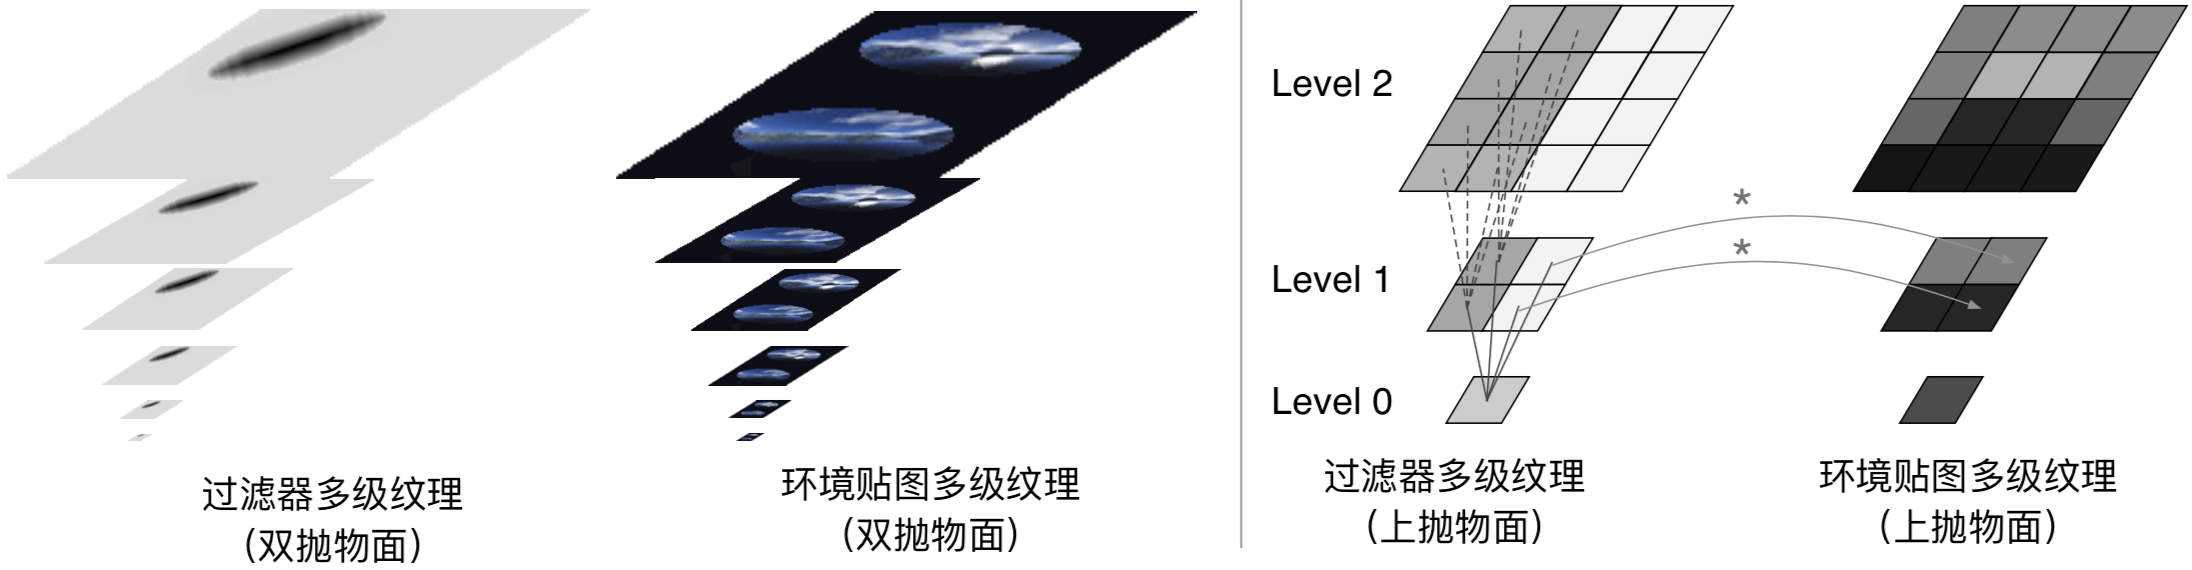
\includegraphics[width=\thewidth]{figures/pl/pre-filtering-4}
	\caption{环境贴图的阶层式预过滤,左一和左二分别是BRDF过滤器核函数和原始环境贴图的多级纹理,右一和右二图解释了阶层式预过滤(对于单个像素)的工作机制;对于过滤器多级纹理中的每一个像素值(其中上下抛物面分 开处理),分别检查它与其下一(更高)级四个相邻像素的差异,如果这些差异均小于某个阈值,则该像素被使用并与环境贴图多级纹理中对应的像素相乘,否则下一级四个相邻的像素被执行相同的检查,最后将所有这些贡献值累加起来形成目标贴图中一个单一的像素值(图片来自 [Kautz et al., 2000])。(图片来自\cite{a:Aunifiedapproachtoprefilteredenvironmentmaps})}
	\label{f:pl-pre-filtering-4}
\end{fullwidth}
\end{figure}

目标贴图中每个像素值的计算过程如下,如图\ref{f:pl-pre-filtering-4}右一右二小图所示,对于每一个过滤器,我们首先从该过滤器多级纹理的最低一级(即第0级)开始,这一级只有一个像素,如图\ref{f:pl-pre-filtering-4}右二小图的第0级,对于该单个像素,首先检查它与下一级(即第1级)相邻4个像素值的差异,如果该差异小于某个阈值,例如0.001,则说明过滤器中的该部分区域比较平滑,因此该低级的过滤器值可以直接被使用,否则更高一级的4个相邻像素被使用。

在图\ref{f:pl-pre-filtering-4}中,第0级与第1级4个相邻像素的差异较大,因此第0级的 像素被抛弃,并用第1级的4个像素值来代替,而这4个像素与第3级纹理中相邻的4个像素的差异值均小于阈值,因此这4个值直接被使用,它们的像素值直接与环境贴图多级纹理中的对应像素值相乘然后被累加到最终结果中。

通过阶层式过滤,过滤器核函数中平滑的部分不必按其实际的像素数量执 行相乘操作,因此加速了预过滤计算,这和本书前面第\ref{chp:rad}章第\ref{sec:r-hierarchical-radiosity}节介绍的阶层 式辐射度方法的原理类似。



\subsubsection{重要性采样方法}
阶层式预过滤是一种非常高效的预过滤方法,它主要通过减少对低频区域内环境贴图的像素读取次数来提高预过滤的效率,这是通过生成一个多级的环境贴图来实现的。然而,为了取得每个BRDF样本对应多级环境贴图的层级,阶层式方法依赖于一个从小向上的递归比较方法,这种递归的算法结构对GPU是非常不友好的,因为相邻的样本递归的次数可能完全不一样,这使得算法的并行性很差,因此原始的阶层式预过滤算法\cite{a:FastArbitraryBRDFShadingforLowFrequencyLightingUsingSphericalHarmonics}是实现于CPU中的。

很显然,在实时渲染中,我们需要能够对GPU友好的算法,这样的算法要求程序具有较高的并行性,本节介绍的重要性采样方法\cite{a:Real-timeShadingwithFilteredImportanceSampling}就是这样一种方法,这种方法保留了阶层式预过滤方法的优点(即使用一个多级环境贴图来减少低频区域内像素的读取次数),同时又具有很好的并行性,能够高效地实现在GPU中。

阶层式过滤方法的缺点在于,它无法预估一个BRDF方向样本的重要性,因此它需要在一个迭代算法结构中通过比较与相邻像素的差异来确定使用什么样的方向样本,以及计算其样本的重要性。给定一个BRDF的显式表述形式,我们可以使用重要性采样方法对其进行采样,如图\ref{f:pl-importance-sampling}(a)所示,然后样本的重要性将用于选择多级环境贴图的层级,如图\ref{f:pl-importance-sampling}(b)所示。

\begin{figure}
	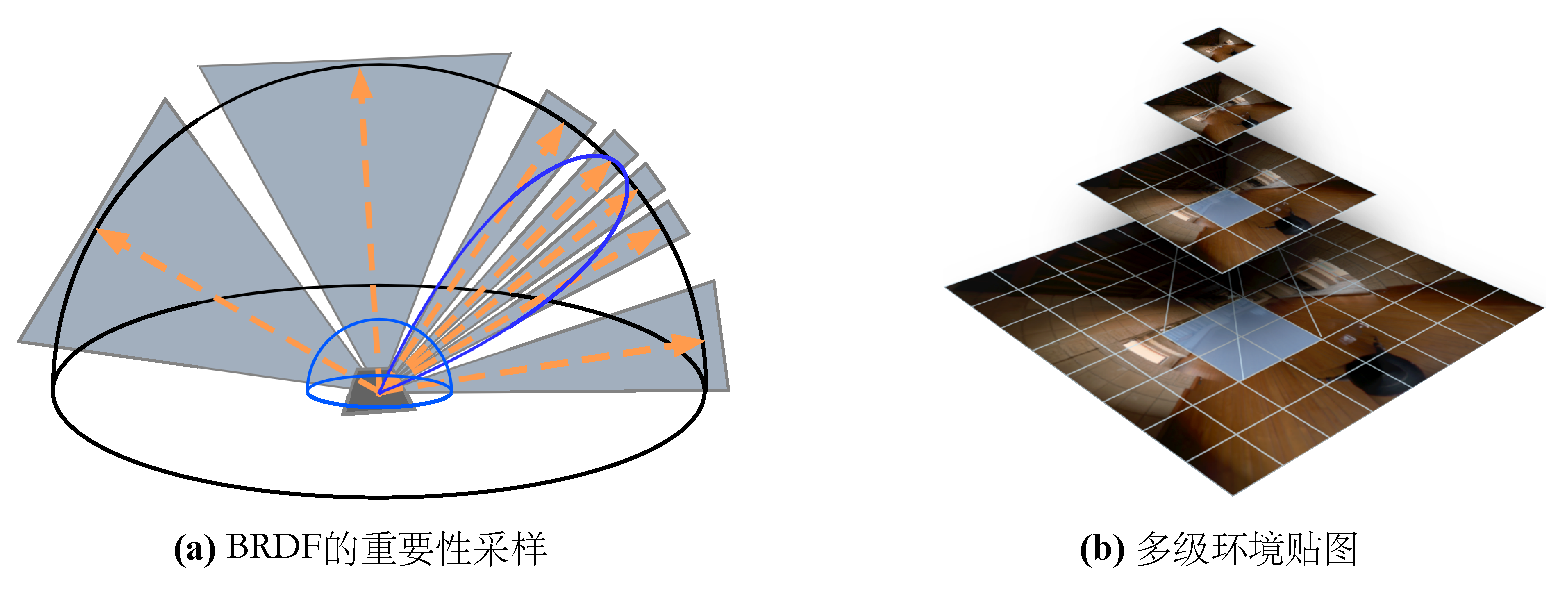
\includegraphics[width=\textwidth]{figures/pl/importance-sampling}
	\caption{重要性采样方法首先对BRDF函数执行重要性采样(b),然后根据样本的重要性来选择对应的多级环境贴图的层级(a),其过滤的窗宽反比于其重要性(图片来自\cite{a:Real-timeShadingwithFilteredImportanceSampling})}
	\label{f:pl-importance-sampling}
\end{figure}

为了对BRDF采样,工业中通常使用一个简化的GGX模型\cite{a:Physically-basedlightingincallofduty:Black,a:Gettingmorephysicalincallofduty:Blackopsii,a:RealShadinginUnrealEngine4},即将式\ref{e:pl-prefiltering-1}拆分成以下两部分:

\begin{equation}
\begin{aligned}
	R(v)=&\int_H L(l)\cfrac{D(h)G(l,v,h)F(V,H)}{4(n\cdot v)}{\rm d}l\\
	\approx&\Biggl(\int_H L(l)D(h){\rm d}l\Biggl)\Biggl(\int_H \cfrac{G(l,v,h)F(v,h)}{4(n\cdot v)}{\rm d}l\Biggl)
\end{aligned}
\end{equation}

上式的第二个积分项可以被预计算起来,因为它们与光照场是无关的。所以剩下的,我们仅需要对微面元的法线分布函数$D(h)$进行采样,这形成下面的预过滤积分形式:

\begin{equation}\label{e:pl-intergal-directional}
	\int_H L(l)D(h){\rm d}l
\end{equation}

对于一个给定的法线分布函数,我们在CPU端生成其使用的方向样本,并将其传输到GPU的常量寄存器中,然后所有使用该法线分布函数的表面都使用这些相同的样本。这些球面空间中相对于表面法线的方向样本,可以通过使用逆变换算法从一对均匀样本$\xi_0,\xi_1\in[0,1]$中生成,即:

\begin{equation}\label{e:pl-uniform-sampling}
\begin{aligned}
	\theta=&2\pi \xi_0\\
	\phi=&\tan^{-1}\Biggl(\cfrac{\alpha\sqrt{\xi_1}}{\sqrt{1-\xi_1}}\Biggl)
\end{aligned}
\end{equation}

\noindent 其中,$\alpha$表示的是表面的粗糙度,这里考虑几何项的重要性,这里每个样本还需要被$|l\cdot n|$加权。

通过上面的方法,我们已经得到了一个方向样本,那么接下来的问题就是怎样选择该样本使用的多级环境贴图的层级。通过观察图\ref{f:pl-importance-sampling}(a),我们可以使用每个样本所“占据”的方向范围来决定该样本所过滤的范围,这个范围进而被用来选择多级纹理的层级,于是我们可以通过每个样本在方向空间所占据的立体角,与环境贴图中每个像素所占据的立体角的比率来计算多级纹理的层级。

样本在方向空间的立体角$SA_{\rm sample}$等于均匀分布样本的尺寸除以每个样本的重要性函数,这是因为每个样本所占据的“范围”与其重要性函数成反比,如图\ref{f:pl-importance-sampling}(a)所示;而每个像素的表面尺寸可以通过如下的方式计算:即立方体每个面的面积4\footnote{每个边的坐标值范围为$[-1,1]$,所以面积为4。},被由方向空间向立方体投影变换的雅可比矩阵$J(x,y,z)$加权,然后再除以每个面内像素的数量$Resolution^{2}$,其中有立方体面$[-1,1]^{3}$向单位球面投影的雅可比矩阵为$J(x,y,z)=\cfrac{1}{(x^{2}+y^{2}+z^{2})^{3/2}}$。综上,样本对应多级纹理的层级可由下式计算得出,即:

\begin{equation}\label{e:pl-lod}
\begin{aligned}
	SA_{\rm sample}=&\cfrac{4\pi}{ND\bigg(\cfrac{p+n}{||p+n||}\bigg)}\\
	SA_{\rm texel}=&\cfrac{4J(p_x,p_y,p_z)}{Resolution^{2}}\\
	MipLevel=&\cfrac{1}{2}\log^2\Biggl(\cfrac{SA_{\rm sample}}{SA_{\rm texel}}\Biggl)
\end{aligned}
\end{equation}

在实现中,有两种策略来执行上述的重要性采样预过滤过程,对于各向同性的BRDF分布函数,我们可以直接在CPU段预计算出每个BRDF分布函数需要使用的样本,然后这些样本被上传的GPU中,表面上的每个像素都执行相同的计算,因此能够符合GPU的并行计算特征,同时能够保留阶层式预过滤方法使用多级环境贴图的优点;对于各向异性的BRDF分布函数,那么方向采样的过程则涉及到表面法线,因此这个重要性采样过程必须发生在GPU阶段,这种情况下CPU只能生成均匀的随机$[\xi_1,\xi_2]$,而包括式\ref{e:pl-uniform-sampling}和\ref{e:pl-lod}的整个过程则均实时发生于GPU端的像素着色器中。

\begin{myshaded}
	尽管阶层式预过滤和重要性采样方法都能够实现对多级环境贴图的像素读取,但是两者的精确度是不一样的。
	
	阶层式预过滤方法由于使用过滤器与环境贴图中像素乘积的值来作为差异比较的依据,这相当于是对整个被积函数进行重要性采样,因此每个样本的贡献值能够最大化。方然这里我们不能说它就一定具有更快的收敛速度,因为它本质上不是一种完全的重要性采样方法,它的每个样本需要通过多次迭代才能最终确定,因此存在一定数量的浪费。
	
	但是反观重要性采样方法,它仅仅是对法线分布函数$D$进行重要性采样,因此当法线分布函数与整个被积函数的形状差异比较大时,其方差就会比较大。
\end{myshaded}




\subsubsection{实时预过滤方法}
重要性采样方法的主要缺点,是它的样本具有随机性,因此整个估计会有比较大的方差,这往往需要使用更多数量的样本才能减少这种估计误差,例如它需要增加4倍的样本数量才能减少2倍的方差。对于GGX而言,它的一个重要特征是在很大的方向范围内存在一个“拖尾”,在这些拖尾的区域,其BRDF分布函数的重要性很低,因此这些拖尾区域的方差会非常高,为了实现这种重要的光泽反射特征,重要性采样方法不得不使用非常大数量的样本,因此使得其很难满足实时预过滤的要求。

重要性采样预过滤方法的误差来源于其使用方向样本的随机性,本节要介绍的也是一种基于重要性采样的方法,但是它通过精心控制这些样本的位置,其影响环境贴图的尺寸,以及样本的权重来最小化这种随机性,从而使得最终的预过滤结果的误差最小。通过减少样本的随机性,整个预过滤估计具有更小的误差,因此在相同的误差条件下,这种方法需要的样本数量相对于重要性采样要少得多,从而使其能够比较好的适用于实时地对环境贴图执行预过滤。

除此之外,前面这些关于预过滤的内容,仅讨论了一般预过滤的原理及方法,并没有针对特定的环境贴图表述形式,这些方法能够很好地作用于球面空间,但是当前工业中大多使用的是立方体贴图,当这些过滤方法作用于立方体环境贴图时,其会遇到一些困难。一方面,这需要考虑立方体贴图各个面之间的缝隙,特别是那些边角的位置,这些地方的过滤需要考虑来自三个面的像素的加权,这种对于三个表面的参数化非常困难;另一方面,即是过滤器核函数在球面上是圆对称的,但是当期投影到立方体表面时,过滤器会变成各向异性的,尽管许多方法能够处理各向异性的过滤器,但是它们均不能满足实时计算的需求。本节介绍的方法将会描述对这些困难的处理。



\paragraph{基本思路}
样本的随机性带来估计的方差,然而怎样在保证重要性采样的前提下,又能使样本的随机性带来的误差最小化,我们需要一种对估计误差形式上的定义。

为了推导出这个误差的公式形式,首先将式\ref{e:pl-intergal-directional}基于方向的积分转变成以下基于面积的积分形式,这样我们将能够在像素区域进行分析:

\begin{equation}\label{e:pl-intergal-area}
\begin{aligned}
	\int L(x)D(x){\rm d}x\approx &\int L(x)B(x){\rm d}x\\
	\approx &\sum_i c_i\int L(x)b_i(x){\rm d}x
\end{aligned}
\end{equation}

在上式中,$B(x)$表示法线分布函数$D(x)$在立方体贴图上的投影,$i$表示多级立方体贴图上的每一个纹素,该纹素对整个积分的贡献为$b_i(x)$。式\ref{e:pl-intergal-area}中,实际上$\sum_i c_ib_i(x)$是对$B(x)$的一个近似,即将将$b_i(x)$看做一个基函数,那么$c_i$就是$B(x)$投影到这些基函数的系数。


通过观察式\ref{e:pl-intergal-area}可以发现,光照场$L(x)$是一个公共因子,因此上式可重组为:

\begin{equation}
	\int L(x)\Biggl| B(x)- \sum_i c_i b_i(x)\Biggl| {\rm d}x \approx 0
\end{equation}

\noindent 然后通过将$L(x)$从上式移除,可以得到一个不依赖于特定光照场的形式\cite{a:Cardinality-constrainedtexturefiltering}:

\begin{equation}\label{e:pl-min-error}
	\int \Biggl| B(x)- \sum_i c_i b_i(x)\Biggl| {\rm d}x \approx 0
\end{equation}

上式说明,我们可以通过选择某组基函数$b_i(x)$,并使得上述积分被积函数的绝对值最小化,来使得整个预过滤估计(即式\ref{e:pl-intergal-area})的误差最小化。

式\ref{e:pl-intergal-area}并没有定义$b_i(x)$的具体形式,$b_i(x)$是环境贴图所在纹理空间上的基函数\footnote{因为$D(x)$已经被投影到立方体贴图所在的纹理空间。},它表示的是第$i$个像素位置处的贡献值。不管$b_i$如何选择,只要能够找到一组系数$c_i$使得式\ref{e:pl-min-error}的值最小化,即可以使得整个预过滤估计的误差最小化。

特别地,如果选择基函数$b_i(x)$为一个$2\times 2$的盒式过滤器(box filter)\myindex{盒式过滤器}{box filter},则在式\ref{e:pl-intergal-area}第二行公式中,被积函数$L(x)b_i(x)$刚好可以表述为将一个盒式过滤器作用与原始的环境贴图,这刚好是我们形成多级环境贴图的过程,因此式式\ref{e:pl-intergal-area}就转化为各个像素位置处投影系数$c_i$与多级环境贴图中纹素值的乘积的和,这仅仅涉及对多级环境贴图的一次三线性查询操作,而系数$c_i$独立于环境贴图,因此它可以被预计算至一个查询表中,最后整个预过滤的实时计算就会的非常简单:两次纹理的查询操作以及相应两项的乘积计算。

有了上述的理论基础,本节介绍的快速预过滤方法\cite{a:FastFilteringofReflectionProbes}的思路就变得很清晰了,为了实现对立方体环境贴图的实时预过滤,这要求算法的结构非常简单,并且对于每个带预过滤像素仅使用很少的样本,算法中对纹理的查询应该尽可能地使用GPU的三线性插值特性。快速预过滤方法将整个过滤卷积计算分成两个通道,以及一个与环境贴图无关的查询表格的预计算:

\begin{itemize}
	\item 在第一个通道,算法首先对原始环境贴图执行过滤以生成一个多级纹理的结构,这个过程和前面的阶层式预过滤和重要性采样方法的思路是一致的,即减少对低频区域像素的读取次数,因为这些样本覆盖这更大的方向范围,原本它们需要从原始环境贴图读取更多数量的纹素。
	\item 在第二个通道,算法组合多级环境贴图中的纹素与样本查询表格中的系数,计算出最终过滤后的环境贴图。
	\item 最后,上述快速预过滤方法的实时计算部分非常简单,基本上仅仅涉及纹素的读取,该过滤过程的大部分操作都被转移到查询表的生成当中,由于查询表示与环境贴图无关的,因此它在一个预处理阶段被执行,并且可以使用非常复杂的方法来减少估计的误差以及提高最终结果的质量。查询表格中存储着每一个方向样本的位置,其对应多级环境贴图中的细分层级,以及该样本的过滤权重值
\end{itemize}

以下,我们分别详细介绍这三个过程及其涉及的一些相关问题。



\paragraph{第一通道:向下采样}
第一个通道的主要目的,是对原始环境贴图执行向下采样以生成多级的环境贴图。纹素的向下采样(down sampling)\myindex{向下采样}{down sampling}就是对周围的相邻纹素执行加权平均来生成低分辨率纹理的过程,通过前面的分析可知,每个相邻像素的加权权重就是我们用于重建过滤器$B(x)$的基函数$b_i(x)$。

传统生成多级纹理的标准方法是使用一个递归的盒式过滤器(box filter)\myindex{盒式过滤器}{box filter},盒式过滤器其实是一个0阶的B样条(B-spline)\mathindex{B样条}{B-spline},它的递推关系(recurrence relation)\myindex{递推关系}{recurrence relation}为$(1/2,1/2)$\cite{a:Apracticalguidetosplines;rev.ed}。

虽然盒式过滤器非常简单并且计算速度很快,但是从这种分段常数基函数(piecewise constant basis)表述的图像中获取的纹素,用在第二通道的组合计算时,其收敛速度会非常慢,因此我们需要一种相邻纹素之间过渡更加平滑的多级纹理。下一个能够被用于2次幂(power-of-two)网格的B样条是二次B样条(quadratic b-spline)基函数,它的递推关系为$(1/8,3/8,3/8,1/8)$,实验发现它能够在收敛速度和质量之间取得最好的平衡。

然而二次方B样条是一个$4\times 4$的张量积,这意味着我们需要对相邻的16个纹素执行加权计算,目前GPU一般并没有提供这种线性插值特性。但是从\cite{a:Fastthird-ordertexturefiltering}中得到启发,我们可以使用4个双线性的样本来计算对16个纹素的加权平均。考虑1D的情形,我们需要对相邻的$s_1,s_2,s_3$和$s_4$这4个纹素执行的加权计算为:

\begin{equation}\label{e:pl-4-weighted-average}
	1/8s_1+3/8s_2+3/8s_3+1/8s_4
\end{equation}

\noindent 对于线性插值函数${\rm lerp}(a,b,t)=(1-t)a+tb$,上述的加权计算可以重写为两个线性插值的和,即:

\begin{equation}
	\cfrac{1}{2}\bigg({\rm lerp}(s_1,s_2,3/4)+{\rm lerp}(s_3,s_4,1/4)\bigg)
\end{equation}

上式说明,我们可以使用两个简单的线性插值计算来计算式\ref{e:pl-4-weighted-average}所示的加权计算,而这种线性插值特性是GPU能够提供的。图\ref{f:pl-downsampling}显式了这种线性插值的图形化描述,其中黑色轮廓线表示位于立方体贴图边角的4个纹素,其中每个纹素的中心位于由蓝色线条构成的网格单元的顶点位置,绿色点线表示立方体面的边,4个红色的原点分别表示4个双线性的样本位置,它们分别位于相邻两个纹素的$1/4$和$3/4$的位置处。

\begin{figure}
	\sidecaption
	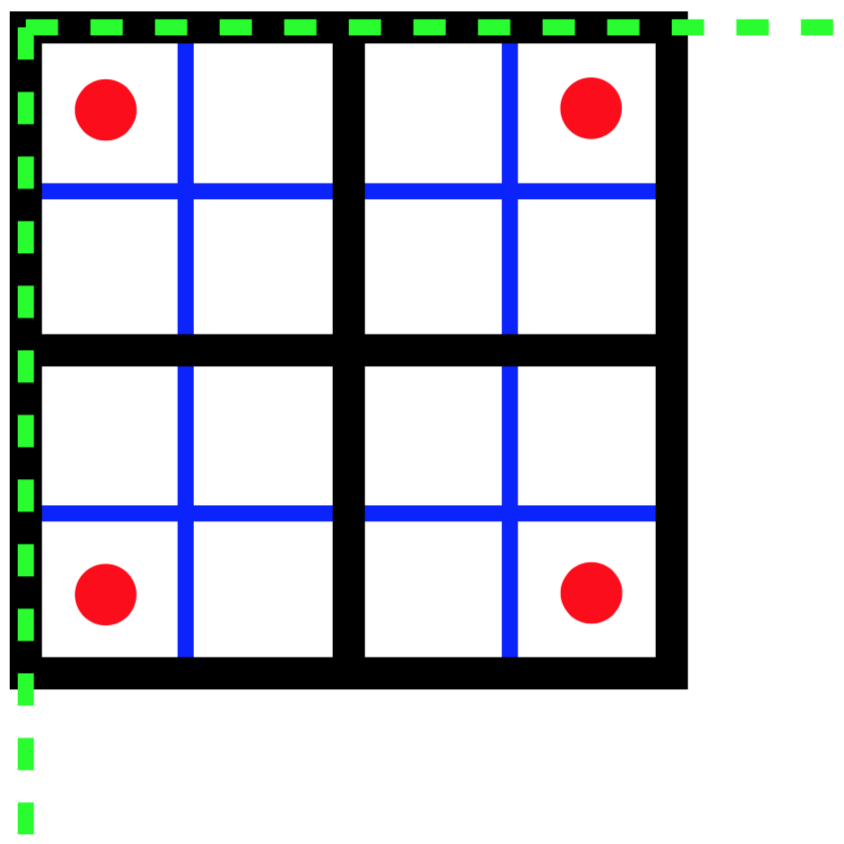
\includegraphics[width=0.3\textwidth]{figures/pl/downsampling}
	\caption{16个样本的二次方B样条加权可以使用4个双线性的样本插值来得到相同的结果}
	\label{f:pl-downsampling}
\end{figure}

另一方面,上述的过滤操作是作用于立方体环境贴图每一个2D的面上的,这也是一般生成多级纹理的方式,过滤器作用于2D的纹理上。然而在本节讨论的快速过滤方法中,我们最终需要将这些二次方B样条的权重值作为法线分布函数的基函数,以更好的近似法线分布函数,如式\ref{e:pl-min-error}所示,而法线分布函数是表述于球面上的,虽然二次方B样条是平滑的,但是球面上一个常数函数投影到立方体的每个面之后,在面与面之间并不是平滑的,所以为了更好地近似法线分布函数,我们需要对递推过程中的每一个样本,使用由球面到立方体表面投影变换的雅可比矩阵$J(x,y,z)$进行加权,这种使用$J(x,y,z)$加权后的$b_i(x)$才能更好地重建法线分布函数。

图\ref{f:pl-reconstruction-comparation}显式了不同的基函数$b_i(x)$在立方体表面上对法线分布函数(本节主要指GGX)的近似,其中盒式过滤器的近似效果比较差,它需要更大数量的方向样本采样比较平滑的近似法线分布函数,如图\ref{f:pl-reconstruction-comparation}(b)所示;图\ref{f:pl-reconstruction-comparation}(c)和(d)均使用了二次方B样条作为基函数$b_i(x)$,但是为加权的二次方B样条不能很好地近似立方体边缘的法线分布函数,如图\ref{f:pl-reconstruction-comparation}(c)所示;而使用雅可比矩阵进行加权的基函数$b_i(x)$能够更好地近似法线分布函数。

\begin{figure}
\begin{fullwidth}
	\begin{subfigure}[b]{0.245\thewidth}
		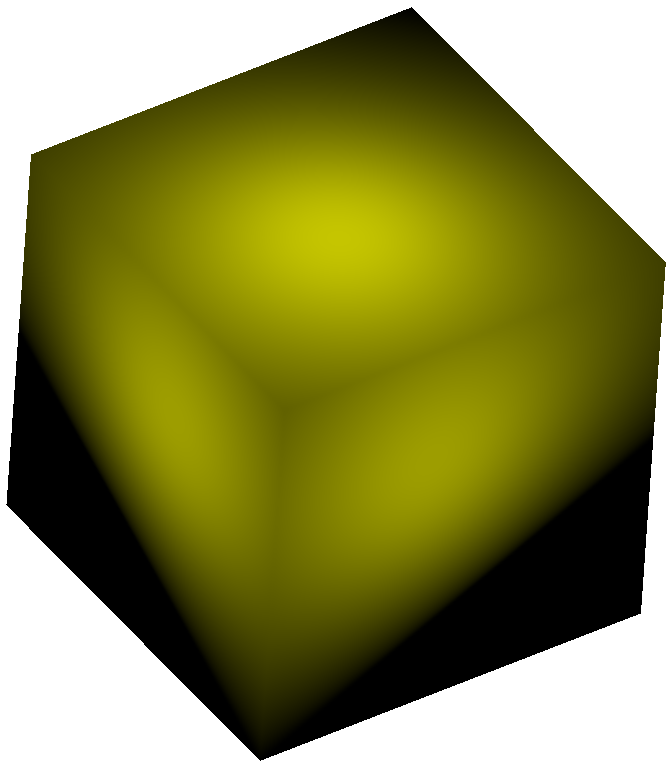
\includegraphics[width=\textwidth]{figures/pl/reconstruction-reference}
		\caption{参考}
	\end{subfigure}
	\begin{subfigure}[b]{0.245\thewidth}
		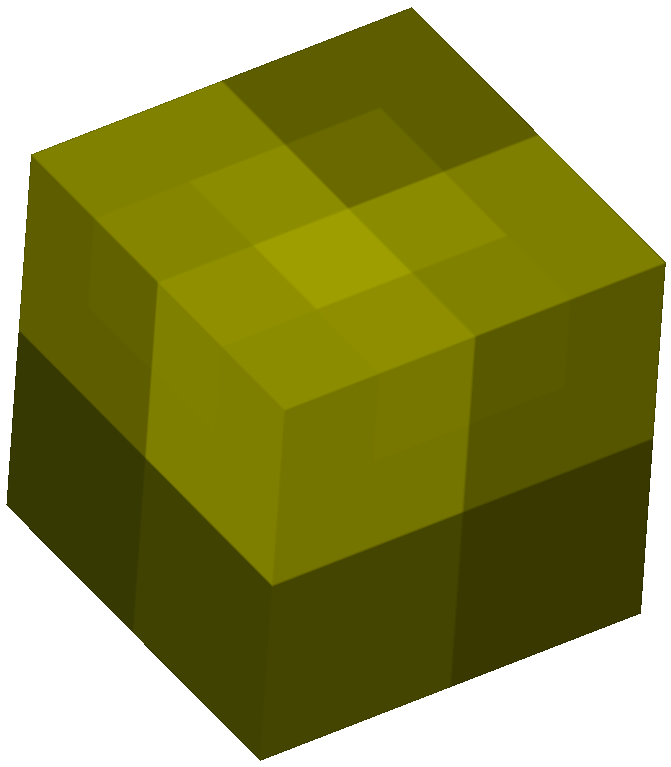
\includegraphics[width=\textwidth]{figures/pl/reconstruction-box}
			\caption{盒过滤器}
	\end{subfigure}
	\begin{subfigure}[b]{0.245\thewidth}
		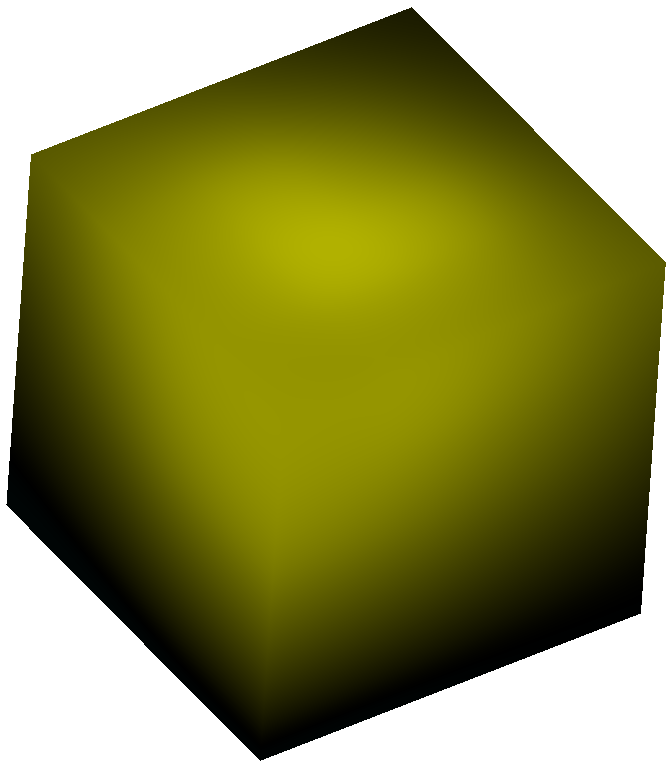
\includegraphics[width=\textwidth]{figures/pl/reconstruction-unweighted}
			\caption{为加权}
	\end{subfigure}
	\begin{subfigure}[b]{0.245\thewidth}
		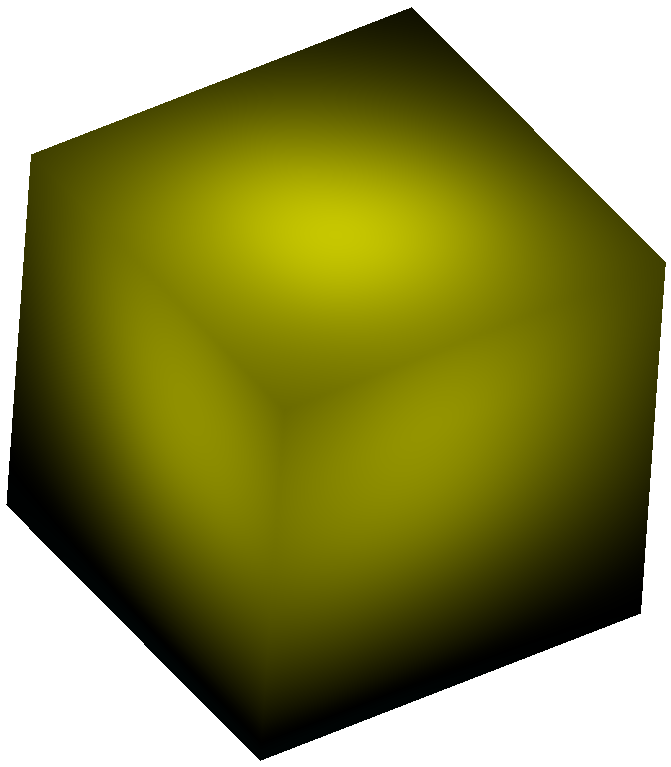
\includegraphics[width=\textwidth]{figures/pl/reconstruction-weighted}
			\caption{雅可比加权}
	\end{subfigure}
	\caption{不同基函数$b_i(x)$对一个粗糙表面的GGX核函数的重建结果,这里对每个像素均使用8个样本进行重建,好的基函数能够大大减少需要的方向样本的数量,提高了精确度并加快了收敛速度(图片来自\cite{a:FastFilteringofReflectionProbes})}
	\label{f:pl-reconstruction-comparation}
\end{fullwidth}
\end{figure}




\paragraph{第二通道:法线分布函数的近似}
第二个通道的主要目的,是将从多级环境贴图中查询的多个三线性样本,与后面预计算的查询表中的系数进行组合,以对最终的预过滤结果进行近似。

前面已经计算出了多级环境贴图中的颜色值,但是还不知道系数表格中的对每个样本到底存储了哪些参数值,以及每个参数的用途是什么,这就是接下来的内容。

对于每一个GGX核函数,其预计算出并存储的系数表格为:

\begin{equation*}
	{\rm Table}=(N \text{个样本})\times(3\text{个坐标系})\times (5\text{个参数值})\times(3\text{个多项式系数})
\end{equation*}

其中$N$为每个GGX核函数使用的方向样本的数量,我们将在后面具体描述怎样确定这些样本的位置,这里先假设它已经被确定;3个坐标系用来进行混合以消除极点,这也会在后面介绍。

其中的5个具体的参数值才是我们最终执行预过滤组合计算需要的参数值,它们分为以下三个数据类型:

\begin{itemize}
	\item \textbf{float3}:一个$<x,y,z>$坐标值,它表示的是样本的位置。
	\item \textbf{float}:样本对应多级环境贴图的细节层级$l_i$。
	\item \textbf{float}:样本的权重,即投影系数$c_i$。
\end{itemize}

样本的位置$<x,y,z>$是相对于一个待计算纹素坐标系$\hat{x},\hat{y},\hat{z}$的偏移值,这个纹素的坐标系定义于一个极坐标系(polar coordinate)中,其中$\hat{z}=\hat{n}$为纹素的方向,$\hat{a}$为极坐标的方向,纹素的正切空间定义为$\hat{x}=normalize(\hat{a}\times \hat{z})$,$\hat{y}=normalize(\hat{a}-\hat{z}(\hat{a}\cdot\hat{z}))$,如图\ref{f:pl-polar-frame}所示。

\begin{figure}
	\sidecaption
	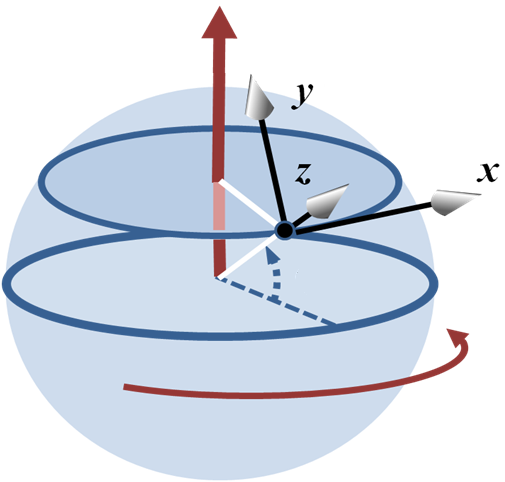
\includegraphics[width=0.45\textwidth]{figures/pl/polar-frame}
	\caption{使用极坐标系来定义样本的偏移位置,在快速预过滤方法中每个样本位置包含三个极坐标系,其极坐标分别对应三个主轴(图片来自\cite{a:FastFilteringofReflectionProbes})}
	\label{f:pl-polar-frame}
\end{figure}

在上述的极坐标系下定义的正切空间中,其在极点$\pm$处会存在奇异值,因此为了避免这种情况,\cite{a:FastFilteringofReflectionProbes}对每个样本位置使用了三个极坐标系,其每个极坐标的方向分别对应三个主坐标主轴,最终的参数值来源于这三个坐标系下参数值的混合,其混合的规则使得这些奇异值位置的混合系数为0,其它完全不与奇异值相交的位置混合系数为1,其它区域则平滑地过度,具体内容参见原文,我们关注于预过滤方法,这里不再对其详细讨论。

现在总结一下以上内容,对于每一个GGX核函数,它有三个极坐标系,其中每个坐标系内有$N$个独立的方向样本,每个样本有5个参数:定义于坐标系$(x_i,y_i,z_i)$内的位置偏移,其使用的细分层级$l_i$,以及样本的权重值$w_i$(即投影系数$c_i$)。每个样本的位置$p$可表示为$p=x_i\hat{x}+y_i\hat{y}+z_i\hat{z}$。

基于以上内容,一个环境贴图每个纹素的预过滤颜色值为:

\begin{equation}
	\cfrac{\sum^{2}_{frame=0}W_{frame}(n)\sum^{N-1}_{i=0}w_i sample(p,l_i)}{\sum^{2}_{frame=0}W_{frame}(n)\sum^{N-1}_{i=0}w_i}
\end{equation}

\noindent 其中,$W_{frame}$为每个极坐标系的加权值,$w_i$即为后面会介绍的法线分布函数的投影系数$w_i$,而函数$sample(p,l_i)$从多级环境贴图中执行三线性插值得到的光照值。

从上式可以看出,实时预过滤方法的实时计算非常简单,它仅仅涉及对多级环境贴图的三线性采样,以及从系数表格中顺序读取各个参数值,所有关于样本位置的采样,以及投影系数的计算均被前置到后面会介绍的预计算阶段,这大大加速了对环境贴图的预过滤计算。

最后,除了通过增加样本的数量,我们还可以根据纹素在立方体表面上的位置来调整这些采样参数的值,使得估计的误差进一步减小,这也是为了更好地考虑核函数由球面空间向立方体表面投影时的不均匀性。\cite{a:FastFilteringofReflectionProbes}简单地将这些采样参数表示为纹素位置的一个低阶的多项式,其中纹素的在立方体中的坐标定义如图\ref{f:pl-polynomials}所示,其中$\theta$为绕极点方向逆时针旋转的角度,它在每个面由-1到1之间线性变化,$\phi$则在每个侧面由下向上在-1到1之间线性变化,并在走向极点时变化至0。

\begin{figure}
	\sidecaption
	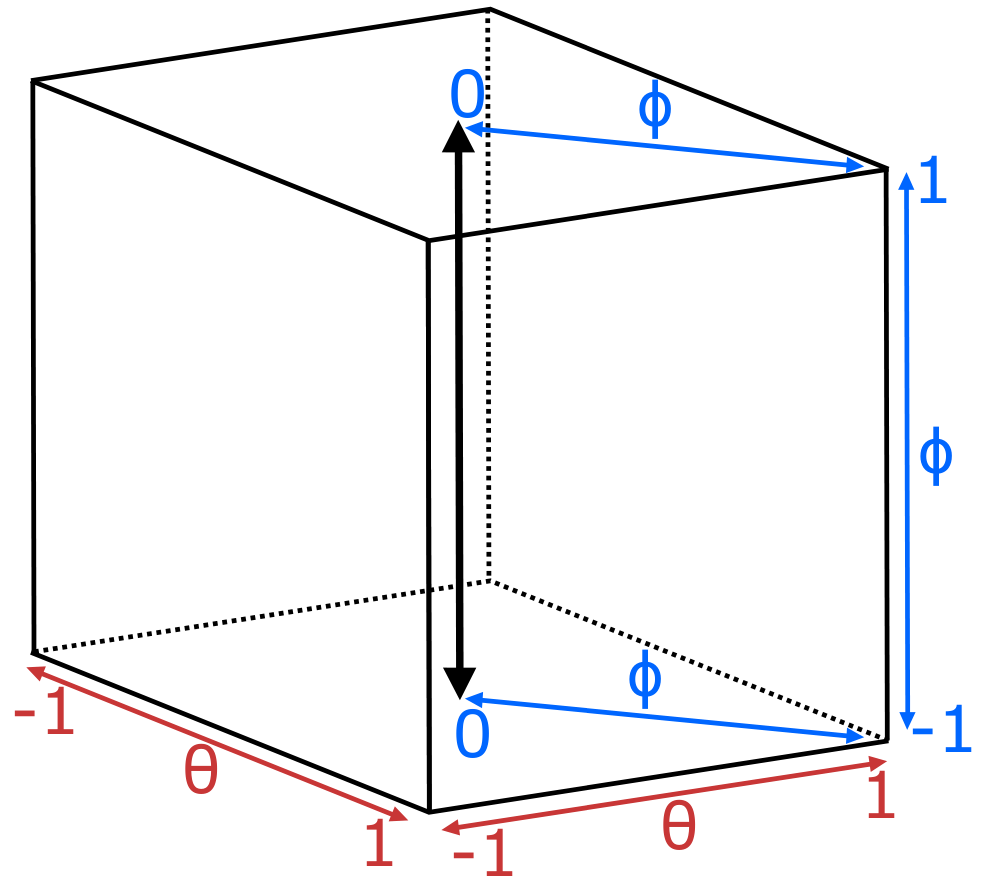
\includegraphics[width=0.47\textwidth]{figures/pl/polynomials}
	\caption{立方体的参数化,其坐标值在每个坐标轴线段上的变化是线性的,其中$\theta$在于垂直边线的交点处会存在不连续,但是$\phi$在底边从-到-1的变化是连续且变化为1,然后从下到上由-1到1的过程中连续变化至0(图片来自\cite{a:FastFilteringofReflectionProbes})}
	\label{f:pl-polynomials}
\end{figure}

基于上述的基础,每个样本的参数相对于纹素位置的函数为:

\begin{equation}
	P(\theta,\phi)=a+b\theta^{2}+c\phi^{2}
\end{equation}

当然处于计算效率的考虑,这只是一个经验上的近似,但是其能够一定程度上减少预过滤结果的误差。



\paragraph{预计算:系数表的优化}
系数查询表格中的参数是在预计算阶段计算的,前面已经介绍了这些参数怎样被用于实时阶段的预过滤计算,现在我们就要来介绍这些参数是怎样生成的。其中前面的内容已经介绍了细分层级$l_i$和多项式系数的计算方法,我们还剩下两个参数值的计算方法没有介绍:即投影系数$c_i$以及每个样本位置的确定。

首先介绍的是投影系数的计算,由于它必须依赖于确定的样本位置,所以首先假设样本的位置已经确定,那么我们需要确保在这些已知的$N$个样本下使得最终预过滤的结果误差最小,本节前面的内容已经介绍过,这即是使得式\ref{e:pl-min-error}所示的积分值最小化,为了便于描述,这里将其公式重写如下:

\begin{equation}\label{e:pl-min-error-1}
	\int \Biggl| B(x)- \sum_i c_i b_i(x)\Biggl| {\rm d}x \approx 0
\end{equation}

上式本质上是一个回归问题,本书在前面第\ref{chp:path-tracing}章第\ref{sec:pt-first-order-regression}节已经介绍过关于回归分析(regression analysis)\myindex{回归分析}{regression analysis}的知识,回归分析通常涉及用一些预测变量(这里是$b_i(x)$)和相应的参数(这里是$c_i$)来表述一个函数(这里是$B(x)$)的形式,通常已知要拟合的函数的形式,我们的目标是要得出相关的这些预测变量对应的参数。

当进行回归计算时,我们首先需要选择相应的损失函数(loss function)\mathindex{损失函数}{loss function},这有两种选择,即L1范数(L1-norm)\mathindex{L1范数}{L1-norm}或L2范数(L2-norm)\mathindex{L2范数}{L2-norm}。

L1范数有称为最小绝对值导数(least absolute deviations,LAD)\mathindex{最小绝对值导数}{least absolute deviations}或者最小绝对值误差(least absolute errors,LAE)\mathindex{最小绝对值误差}{least absolute errors},设目标函数值$y_i$与估计值$f(x_i)$的绝对值为$|y_i-f(x_i)|$,则最小绝对值导数发的目标是要使下述的$S$值最小化:

\begin{equation}
	S=\sum^{n}_{i=0}|y_i-f(x_i)|
\end{equation}

L2范数又称为最小二乘法(least squares)\mathindex{最小二乘法}{least squares},设目标函数值$y_i$与估计值$f(x_i)$的差异为$y_i-f(x_i)$,则最小二乘法的目标是要使得下述的$S$值最小化:

\begin{equation}
	S=\sum^{n}_{i=1}(y_i-f(x_i))^{2}
\end{equation}

尽管最小二乘法是更简单也更常用的回归分析方法,但是\cite{a:FastFilteringofReflectionProbes}发现其对GGX“拖尾”部分的近似能力比较差,而L1范数则能取得更加满意的结果,虽然其计算成本更高,但是由于系数表参数的计算发生在预处理结算,所以这种成本是可接受和值得的。

快速过滤方法的一个重要目标是对样本的位置进行调整,使其分布更加均匀来减少样本的随机性,进而减少估计的误差。然而,要对传统的重要性采样得到的样本的位置进行调整,并使得调整后的估计误差更小是很困难的,但是在\cite{a:FastFilteringofReflectionProbes}中,这里通过对调整后的样本位置来拟合相应的系数,所以它总是能够保证对于给定的样本位置,其估计的误差最小。

快速预过滤方法首先通过传统的重要性采样\cite{a:Real-timeShadingwithFilteredImportanceSampling}方法来得到样本的初始位置,然后通过类似\cite{a:OnthelimitedmemoryBFGSmethodforlargescaleoptimization}的方法来对样本的位置进行调整,使其位置分布更加均匀,如图\ref{f:pl-sampling-comparation}所示。尽管这些位置调整的算法非常复杂,但是由于它们也是发生于预处理阶段,因此不会对实时的预过滤计算造成影响。

\begin{figure}
\begin{fullwidth}
	\begin{subfigure}[b]{0.325\thewidth}
		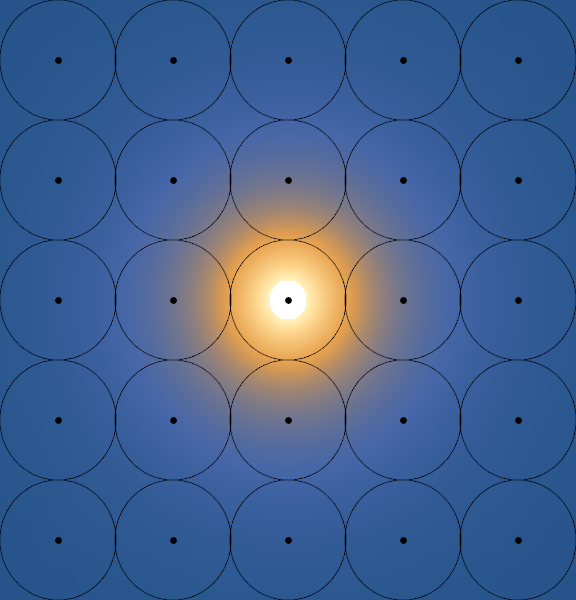
\includegraphics[width=\textwidth]{figures/pl/sampling-raster}
		\caption{光栅化方法}
	\end{subfigure}
	\begin{subfigure}[b]{0.325\thewidth}
		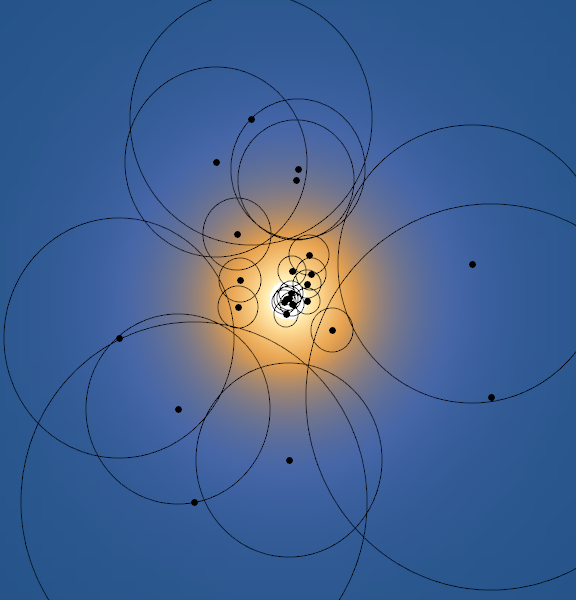
\includegraphics[width=\textwidth]{figures/pl/sampling-importance}
			\caption{重要性采样}
	\end{subfigure}
	\begin{subfigure}[b]{0.325\thewidth}
		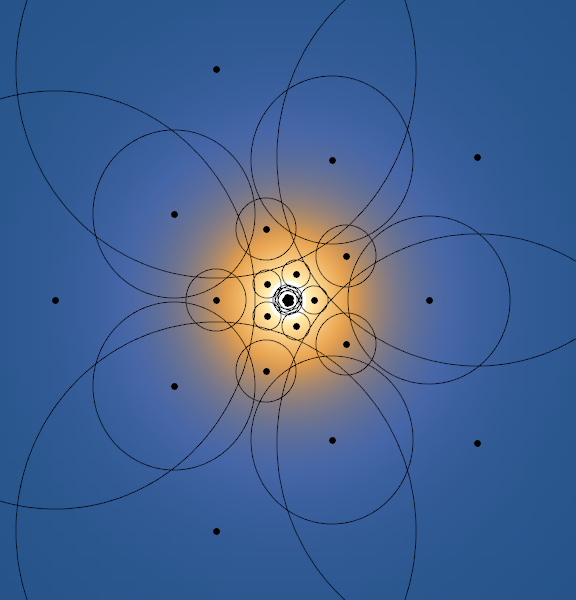
\includegraphics[width=\textwidth]{figures/pl/sampling-optimized}
			\caption{优化的重要性采样}
	\end{subfigure}
	\caption{三种不同采样方法,光栅化方法(a)对整个球面空间进行均匀采样,重要性采样方法(b)则根据法线分布函数进行重要性采样,快速预过滤方法(c)首先使用重要性采样方法生成初始位置,然后对这些样本的位置进行调整,使其分布更加均匀(图片来自\cite{a:FastFilteringofReflectionProbes})}
	\label{f:pl-sampling-comparation}
\end{fullwidth}
\end{figure}





\section{预计算辐射传输}\label{sec:pl-prt}
在场景渲染的每一帧中,渲染方程都要计算光照传输,它是光子从光源发出然后通过场景中的表面最后到达摄像机的过程,如果场景是完全静止的,那么这样的计算过程对于每一帧是相同的,因此我们可以将这个“传输过程”提前计算并缓存起来,这样可以达到较高的实时性能。

预计算辐射(亮度)传输(precomputed radiance transfer,PRT)\myindex{
预计算辐射传输}{precomputed radiance transfer}\cite{a:PrecomputedRadianceTransferforRealTimeRenderinginDynamicLowFrequencyLightingEnvironments}的主要原理,就是上述的光照积分可以被分离为一个包含自阴影和内部反射的预计算传输函数,以及运行时与之组合的一个实时动态改变的环境光照贴图,为了实现这个目标,传输函数和环境光照都被投影到一个正交基函数(例如球谐函数或小波函数),因此原始的光照积分被转化为这些基函数系数的内积,其中环境贴图的系数可以实时修改,而传输函数的系数则被存储于物体表面,因此光照传输只需要计算一次,大大提高了静态场景的渲染效率。

另一方面,因为必须使用很少的系数来表述光源和预计算的数据(矢量或矩阵),所以预计算辐射传输方法的另一个假设是方向函数(光源和传输函数)是低频的,这可以减少内存的占用以及运行时的点积计算,但这也意味着预计算辐射传输仅能处理很柔和的阴影。不过,在该方法的演化中,其它一些方法(例如基于小波的方法)被引入使之能够处理全频率的方向函数。

尽管预计算辐射传输方法比较高效,但是其仅限于静态场景,这大大限制了其运用与发展,所以本章仅对其做简要介绍(不过这并不意味着我们可以完全忽视它,作为一种重要的解决全局光照的思路,还是很有必要对其进行简单地了解,并且它所涉及的关于球谐函数的知识对于后面的辐射照度缓存也是想通的)。首先我们会简要复习一下相应的数学基础知识,然后介绍漫反射表面下的预计算辐射传输,最后将其扩展到一般(如光泽)表面情形,以及对高频函数的处理。



\subsection{漫反射表面的PRT}
为了更直观地理解预计算辐射传输方法的思路,本节我们先讨论最简单的漫反射表面的预计算辐射传输,然后在后续的内容中将其扩展至光泽表面以及全频率光源。

首先我们从渲染方程的纽曼级数展开中的直接光照项开始,即:

\begin{equation}
\begin{aligned}
	L(p\to\vec{d})=&L_0(p\to\vec{d})+L_1(p\to\vec{d})+\cdots \\
	L_0(p\to\vec{d})=&\int_\Omega f_r(p,\vec{s}\to\vec{d})L_{env}(\vec{s})V(p\to\vec{s})H_{N_p}(-\vec{s})d\vec{s}
\end{aligned}
\end{equation}

对于漫反射物体,向各个方向反射的光照是相同的,所以出射辐射亮度是与观察方向无关的,这也意味着BRDF函数是与方向无关的,因此它可以从积分中提取出来,上式中的直接光照项可以重写为:

\begin{equation}\label{e:pl-diffuse}
	L_0(p)=\frac{\rho_d}{\pi}\int L_{env}(\vec{s})V(p\to\vec{s})H_{N_p}(-\vec{s})d\vec{s}
\end{equation} 

\noindent 其中,$\rho_d$表示表面的漫反射系数,它的值介于$0$到$1$之间,分母$\pi$用于保证能量守恒。上式同时假设光源位于无限远处,因此入射辐射亮度与位置无关,而仅与方向$s$有关。

图\ref{f:pl-diffuse}展示了预计算辐射传输的基本思路,左边一列包含了式\ref{e:pl-diffuse}中的三个方向函数,即光源,可见性以及余弦项,预计算辐射传输中的一个特殊处理就是将可见性和余弦项的卷积计算放在预处理过程中,由于卷积计算的结果仍然是一个方向函数,该方向函数被投影为由球谐函数系数构成的矢量并存储起来。最后,在运行时阶段,预存的光照传输矢量和光源的投影系数矢量进行点积计算得出最终的光照积分值。

\begin{figure}
	\sidecaption
	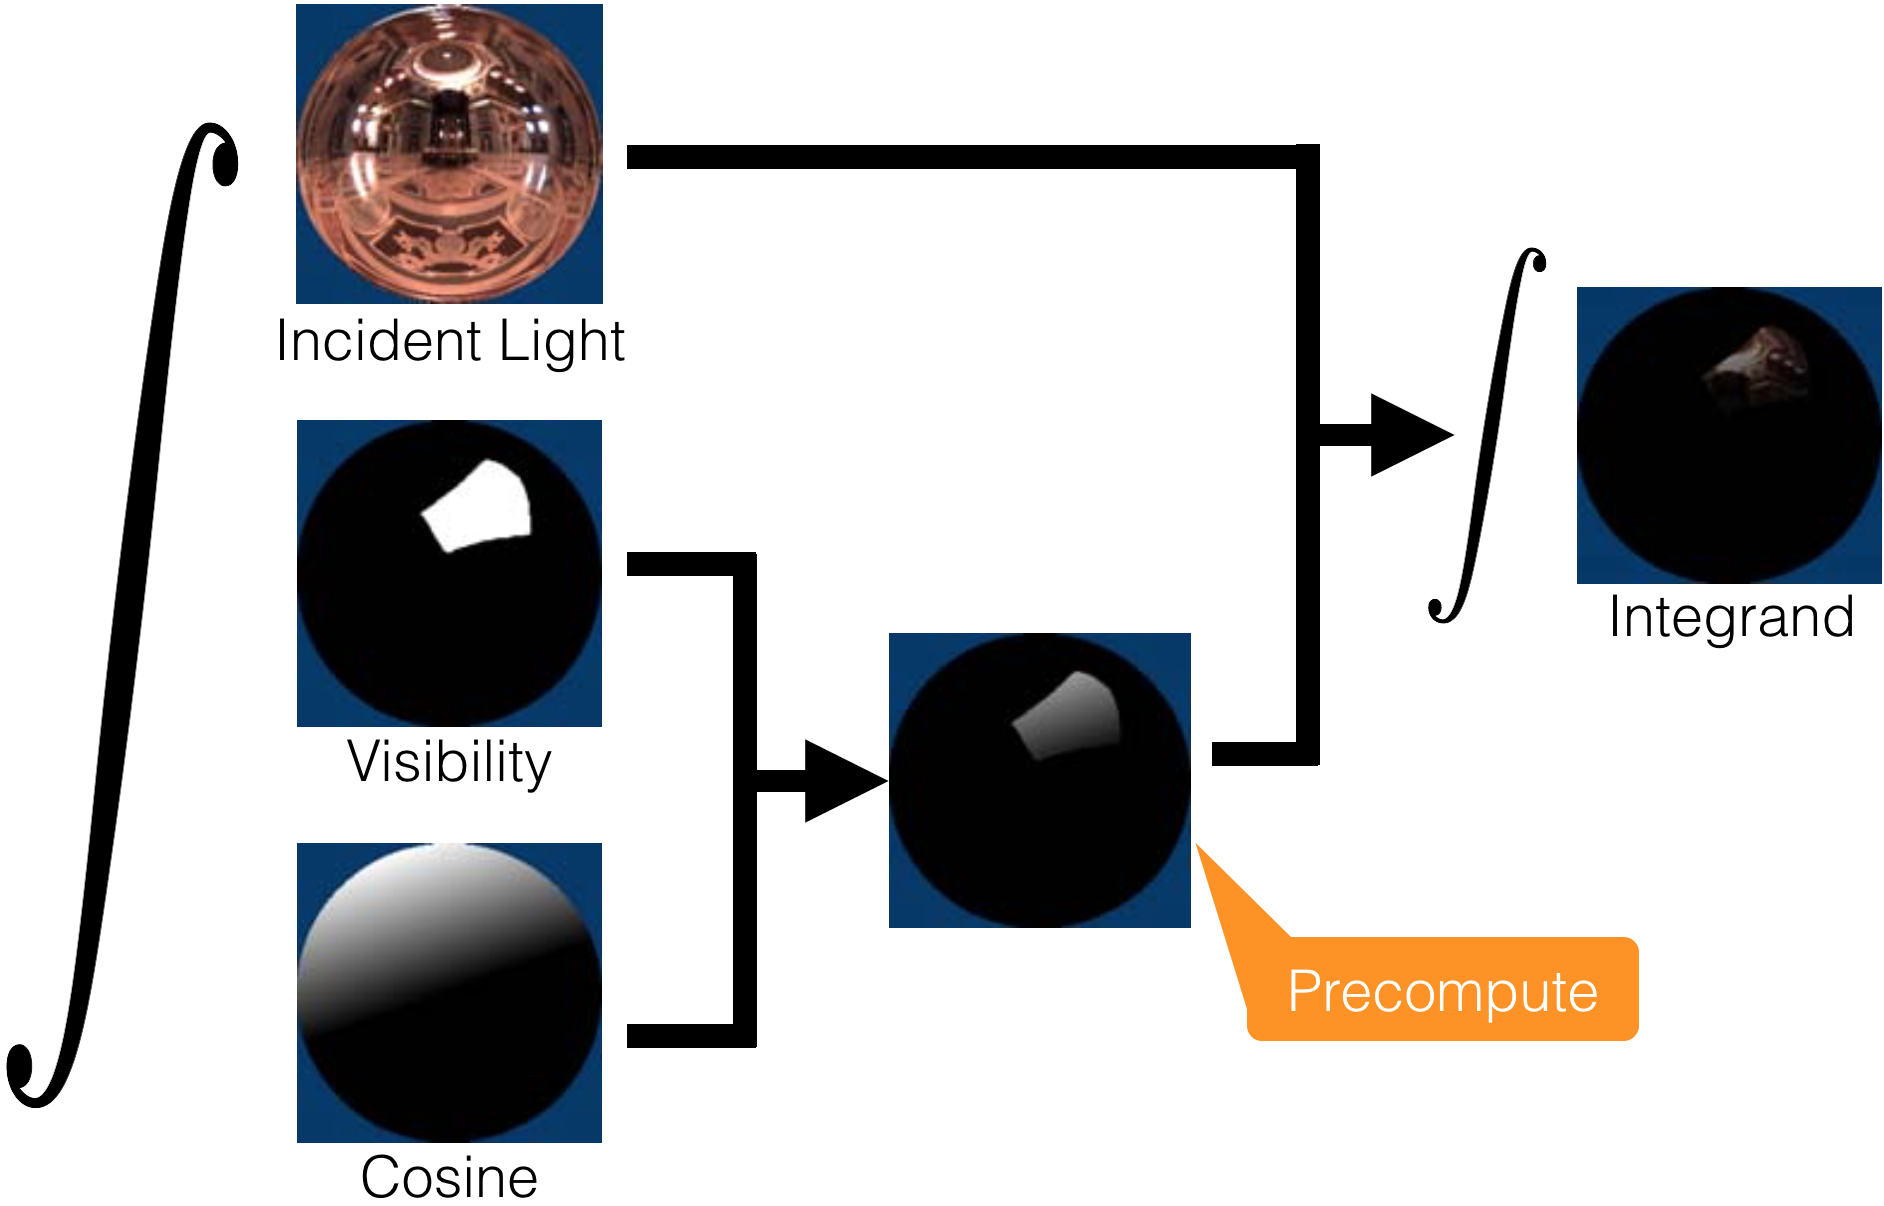
\includegraphics[width=0.65\textwidth]{figures/prt/prt-7}
	\caption{预计算辐射传输的一个主要技巧,就是将可见性和余弦项组合成一个方向函数,然后这个组合的方向函数与入射环境光照的卷积就可以转换为两个球谐函数系数的点积计算,而组合的方向函数则可以被预计算并存储在表面上的每一个位置处,而环境贴图可以动态改变}
	\label{f:pl-diffuse}
\end{figure}

在实时渲染阶段,光源$L_{env}$可以被看做一个未知函数,而余弦加权的可见性或者说传输函数则是已知的,首先我们将入射光照场$L_{env}$投影到球面上,即:

\begin{equation}
	L_{env}(\vec{s})\approx\sum_{i}l_iy_i(\vec{s})
\end{equation}

\noindent 这里$l_i$表示环境光照投影系数,$y_i$则为球谐基函数,根据前面的知识,该系数可以通过求环境光照与每个球谐基函数函数乘积的积分来计算。

将上式直接代入到式\ref{e:pl-diffuse}中,由于被积函数是线性的,因此我们可以将加和与积分符号进行交互,这形成如下的形式:

\begin{equation}
	L_0(p)=\frac{\rho_d}{\pi}\sum_i l_i\int_{\Omega}y_i(\vec{s})V(p\to\vec{s})H_{N_p}(-\vec{s})d\vec{s}
\end{equation}

在上式中,由于积分中的项均是独立于光源的,因此它们可以被预计算起来。其中的积分表示的是一个传输系数,它表述的是入射光照$l_i$怎样被映射为位置$p$处的一个出射辐射亮度值,因此所有传输系数就形成一个传输矢量,该矢量将入射光照映射为出射辐射亮度,即:

\begin{equation}
	L_0(p)=\frac{\rho_d}{\pi}\sum_i l_i t^{0}_{pi}
\end{equation}

\noindent 在上式中,我们可以将漫反射系数合成进传输矢量中,即:

\begin{equation}
	L_0(p)=\sum_i l_i t^{0}_{pi}
\end{equation} 

与上述相似的过程可以被用于其它二次以上的光照反弹,所以表面上每个点处最终的传输矢量就是多个单次反射传输矢量的加和,它可以将任意入射光照映射为出射光照,所以最终的出射辐射亮度就是光源的投影系数与最终传输矢量的点积,即:

\begin{equation}
	\begin{aligned}
		L(p)=&\sum_i l_i(t^{0}_{pi}+t^{1}_{pi}+\cdots)\\
		    =&\sum_i l_i t_{p,i}
	\end{aligned}
\end{equation}

在运行时,我们需要能够查询到表面上每一个像素位置处的传输矢量,然后在顶点/像素着色器执行点积计算,最终的结果就是该像素位置处的入射辐射亮度。




\subsection{一般表面的PRT}
由于漫反射表面的出射光照是一个标量,因此传输函数可以被近似为一个矢量。然而光泽表面的出射光照却是与视觉相关的,即它的出射光照是另一个方向分布函数,这看起来就是两个不同坐标系之间的线性变换,因此我们可以寻找一个变换矩阵,它可以将某个点处的入射光照线性变换为出射光照。



\subsubsection{传输函数}
尽管正如上面的分析,我们可以为表面上的每个点计算一个传输矩阵,这就像对漫反射表面上的每个点计算一个传输矢量一样,然后在运行时对入射环境光照$L_{env}$执行这个传输矩阵的线性变换,最后获取观察方向的出射光照值即可,但是这样的方法有个很大的问题。

对表面点计算传输矩阵的主要问题是,随着表面点空间位置的变化,入射光照场的变化通常很小,因为这些入射光照通常是受整个场景的影响;然而随着表面点位置的变化,像素的入射光照的变化频率则可能很大,比如在那些阴影边界附近的像素,以及那些物体边缘附近的像素,因为出射光照仅受物体自身或者局部的影响。

因此,如果我们考虑的是入射光照与出射光照之间的传输矩阵,则这个传输矩阵的维度需要特别高,也即入射环境光照需要使用更高维度的球谐函数(更多数量的系数)来近似,因为出射光照需要很高的采样频率。尽管这是可行的,但是由于每个表面位置都需要存储整个传输矩阵,因此它不仅影响着内存的占用,还大大增加了着色时的矩阵元素计算量。

所以,鉴于上述原因,考虑到入射光照与出射光照之间不同的变化频率,在实践中,我们将BRDF分布函数从传输函数中提取出来,使传输矩阵仅包含可见性部分,该传输矩阵将入射环境光照变换为表面像素处“看得见”的入射光照分布,最后在实时渲染时,首先将入射环境光照变换为表面像素处的局部入射光照,然后该局部入射光照与表面的BRDF分布函数进行点积计算,以计算最终的入射光照,此时BRDF分布函数可以选择使用更高的采样频率。

\begin{myshaded}
	读者可能会有这样的疑问:入射光照到出射光照之间的变换为什么是线性的呢?
	
	请特别注意,这里的变换其实不是针对空间方向的变换,而是对一个球谐函数的系数执行的变换,因此它实际上是针对每一个相同的球谐函数,将其系数由一个值变换为另一个值,本节的传输函数的线性变换是指这种意义上的线性变换,读者在理解后面的内容的时候尤其要注意。
\end{myshaded}




\subsubsection{转移入射辐射照度}
什么是$p$点的局部入射光照呢?我们称这个量为转移入射辐射照度(transferred incident radiance)\myindex{转移入射辐射照度}{transferred incident radiance}$L_{xfer}(p\leftarrow \omega)$,它表示的是在给定的环境光照$L_{env}$的情况下,点$p$看到的入射光照分布是什么,这既包括直接来自环境光照$L_{env}$的光照(即直接光照),也包括来自其它物体表面反射过来的光照(即间接光照),如图\ref{f:pl-transfer-incident-radiance}(a)所示。

\begin{figure}
	\begin{subfigure}[b]{0.505\textwidth}
		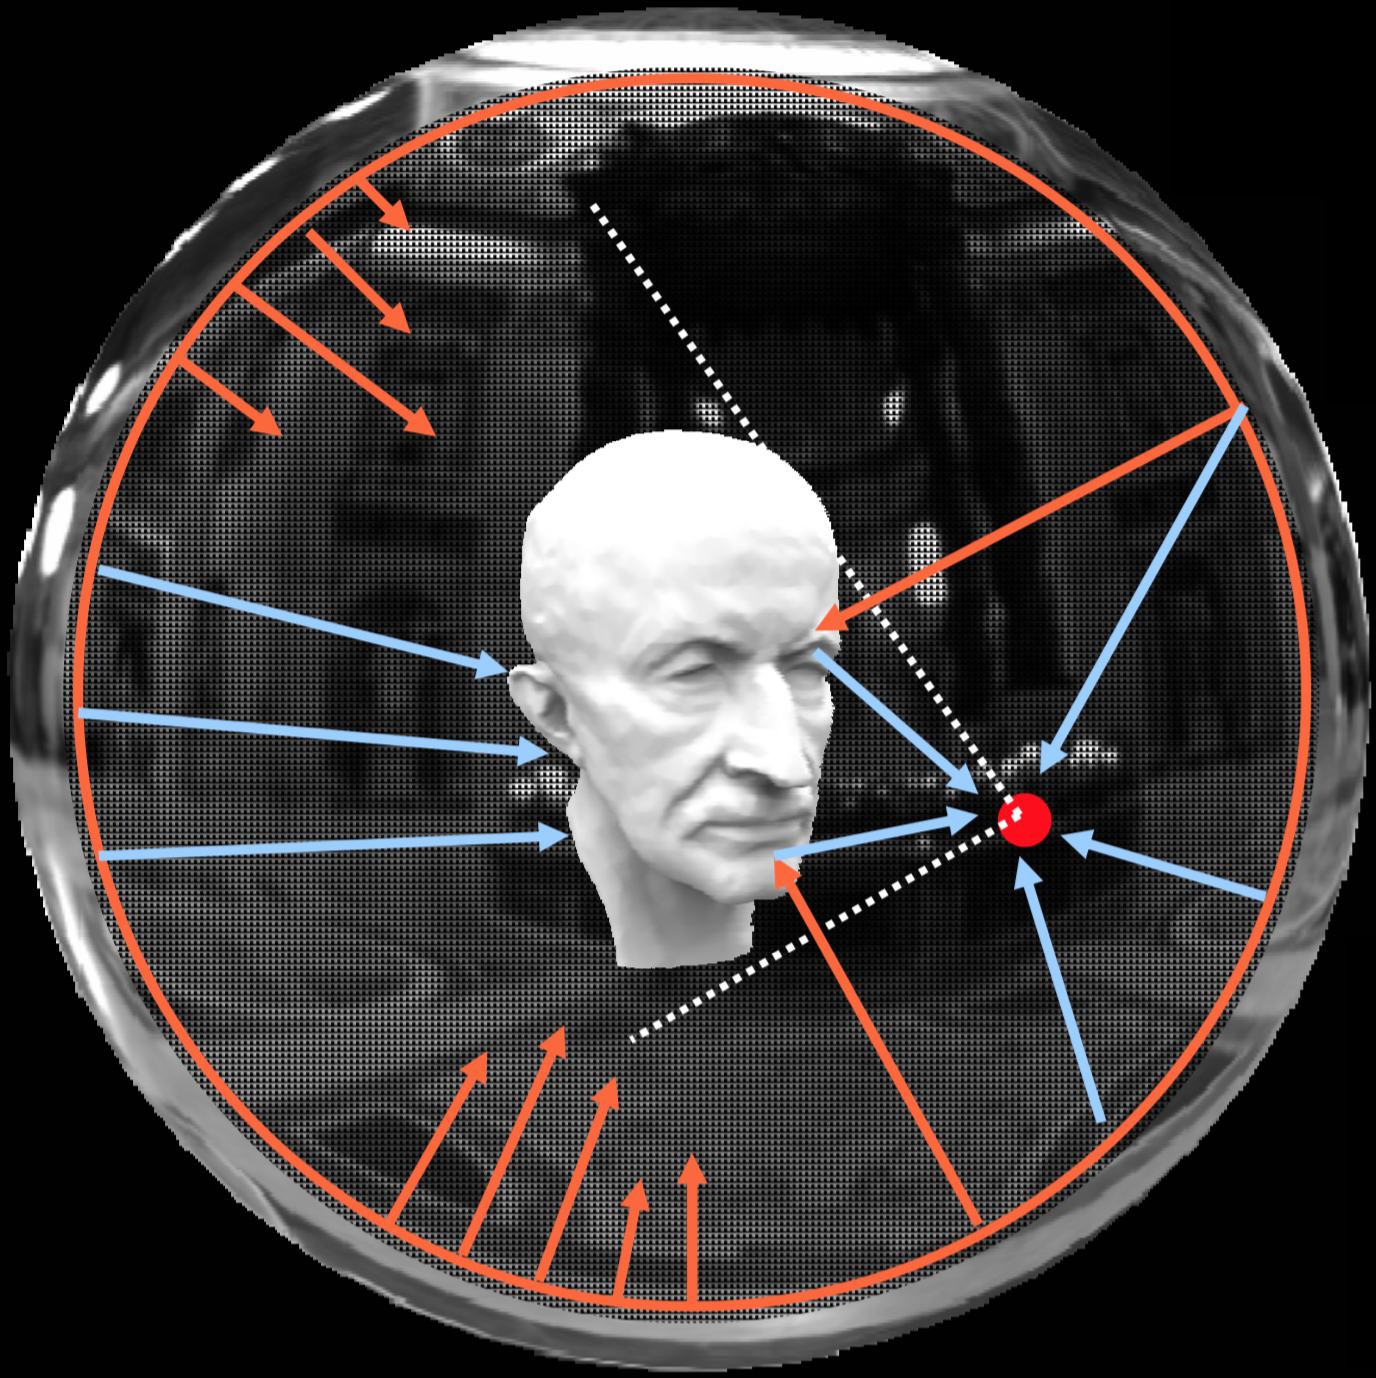
\includegraphics[width=\textwidth]{figures/prt/prt-8-2}
		\caption{$L_{xfer}(p\leftarrow \omega)$的定义}
	\end{subfigure}
		\begin{subfigure}[b]{0.495\textwidth}
		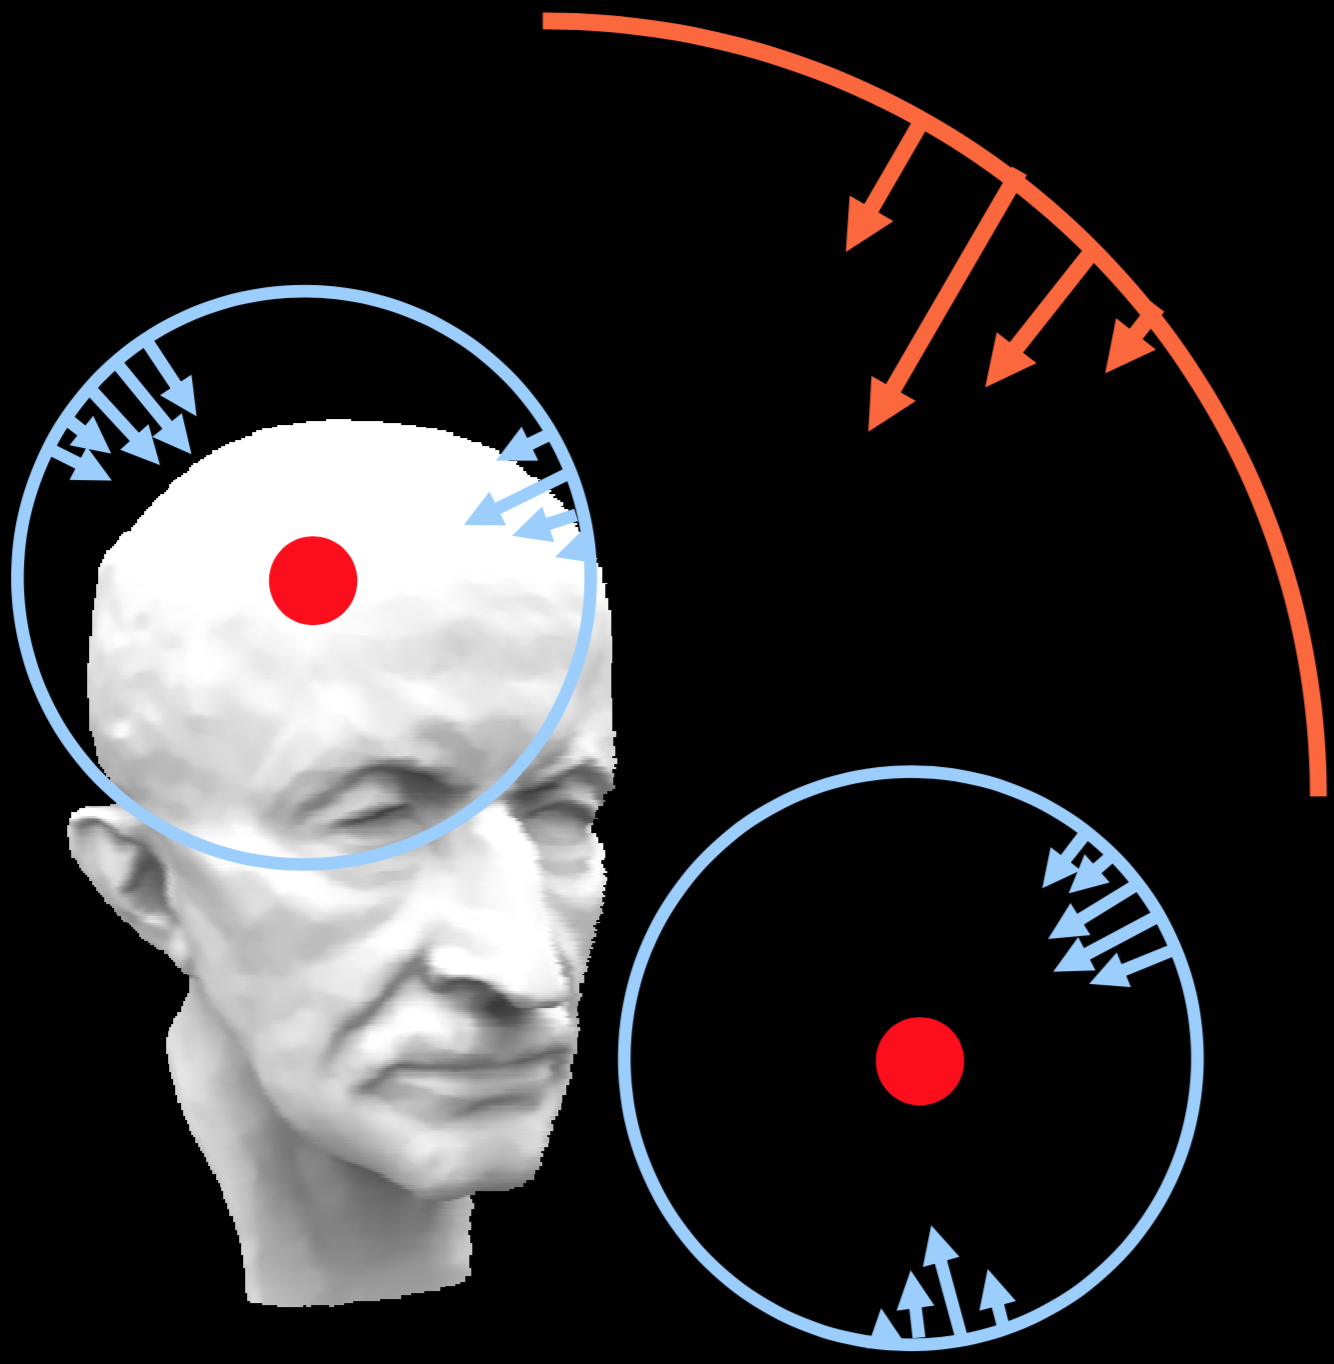
\includegraphics[width=\textwidth]{figures/prt/prt-9}
			\caption{表面和空间位置的$L_{xfer}(p\leftarrow \omega)$}
	\end{subfigure}
	\caption{转移入射辐射照度的定义(a),它表示在给定入射环境光照的情况下,在经历光与表面的反射之后,最终进入点$p$的入射光照分布,其中在PRT方法中,我们同时存储表面和空间位置处的转移入射辐射照度(b),后者可以用于动态物体的光照计算(图片来自\cite{a:PrecomputedRadianceTransfer:TheoryandPractice})}
	\label{f:pl-transfer-incident-radiance}
\end{figure}

除了计算表面位置处的转移入射辐射照度,PRT方法还同时存储离表面很近的空白空间位置处的转移入射辐射照度,如图\ref{f:pl-transfer-incident-radiance}(b)所示,这些来自空间中的入射光照分布可以用于对动态物体执行全局光照技术。

环境光照与转移入射辐射照度之间的关系是线性的,当然前面已经说明这种线性关系是指在相同结束的球谐函数空间下的,即环境光照和点$p$的转移入射辐射照度都被投影到相同阶数的球谐函数空间。因此,环境光照与转移入射辐射照度之间的关系就可以被表述为一个矩阵,这个矩阵一般随着$p$点位置的变化而变化,即:

\begin{equation}
	L_{env}(\omega)\to L_{xfer}(p\leftarrow\omega)
\end{equation}

本节后面,我们的主要目标就是要计算出这个环境光照到转移入射辐射照度之间的变换矩阵,这个变换矩阵可以被预计算并存储在每个点$p$处。

有了关于传输矩阵的计算方法,PRT的算法过程可以总结如下:

\begin{enumerate}
	\item 首先,在离线阶段预计算表面各个点处的传输矩阵。
	\item 然后,在运行时利用传输矩阵计算出$p$点的转移入射辐射亮度$L_{xfer}$。
	\item 最后,计算$L_{xfer}$与余弦加权的BRDF分布函数乘积的积分,以计算出最终观察方向的出射辐射亮度。
\end{enumerate}



\subsubsection{传输矩阵的推导}
为了推导出由环境光照向转移入射辐射照度的转移矩阵,我们首先将转移入射辐射照度投影到有限的球谐函数空间,为了与其它步骤的球谐函数命名冲突,记这里的球谐函数为$\{z\}$。这即是说我们将转移入射辐射照度离散化,并用一些有限个球谐函数的系数$l^{p}$来表述该转移入射辐射照度,如图\ref{f:pl-tir-projection}所示。

\begin{figure}
\sidecaption
	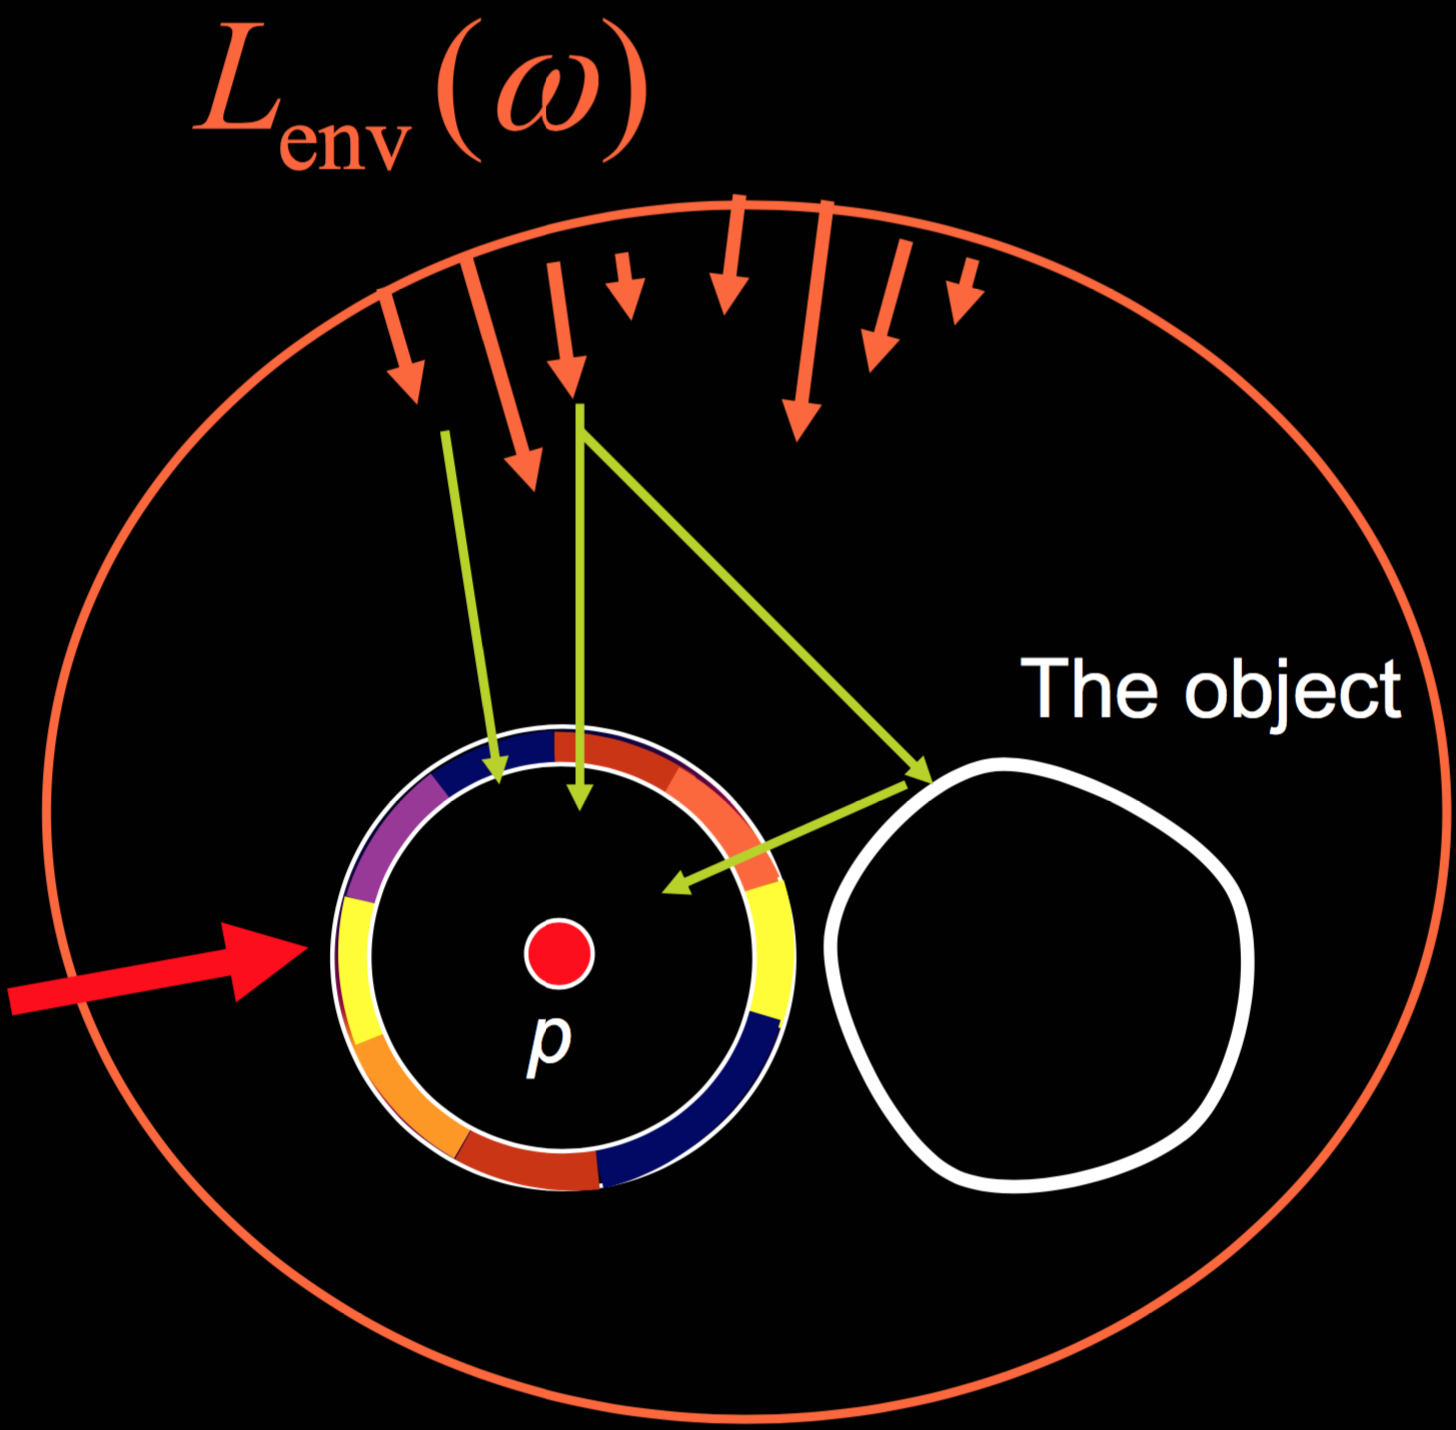
\includegraphics[width=0.5\textwidth]{figures/prt/prt-10}
	\caption{将$p$点的转移入射辐射照度投影到球谐函数空间,这形成一个离散的函数系数表述,注意这里并不是空间位置上的离散化,图示的空间分割仅是为了演示方便,这里每个离散化的片段表述的是一个特定阶数的球谐函数的近似(图片来自\cite{a:PrecomputedRadianceTransfer:TheoryandPractice})}
	\label{f:pl-tir-projection}
\end{figure}

因此$p$点的转移入射辐射照度可以表述为:

\begin{equation}\label{e:pl-transfer-incident-radiance}
	L_{xfer}(p\leftarrow\omega)\approx\sum^{m}_{i=1}l^{p}_{i}z_i(\omega)
\end{equation}

上式说明,我们可以使用一个由各个球谐函数$\{z_j\}$的系数$l^{p}_j$构成的矢量$\mathbf{l}^{p}$来近似$p$点的转移入射辐射照度;同样,环境光照$L_{env}$也可以使用由球谐函数$\{y_i\}$的系数$l_i$构成的矢量$\mathbf{l}$来近似。

由于定义转移入射辐射照度的系数矢量$\mathbf{l}^{p}$是未知的,而定义环境光照的系数矢量$\mathbf{l}$则是已知的,我们需要做的事情就是找到它们两者之间的关系。由于它们两者之间的关系是线性的,因此可以被表述为一个矩阵,我们称之为$p$点的传输矩阵(transfer matrix)\myindex{传输矩阵}{transfer matrix},即:

\begin{equation}
	\mathbf{l}^{p}=\mathbf{T}^{p}\mathbf{l}
\end{equation}

在具体推导这个传输矩阵之前,让我们来分析一下它的意义:假设环境光照只投影到其中一个球谐基函数$y_i$上,并且其系数$l_i=0$,这即是说在矢量$\mathbf{l}$中只有第$i$个元素的值为1,其它元素的值均为0,如图\ref{f:pl-matrix}右边灰色条中白色的小方块所示,考虑矩阵和矢量相乘的定义,它最终的结果就是将矩阵$\mathbf{T}^{p}$中的第$i$列复制出来,这形成图\ref{f:pl-matrix}左边的矢量$\mathbf{l}^{p}$。

\begin{figure}
\sidecaption
	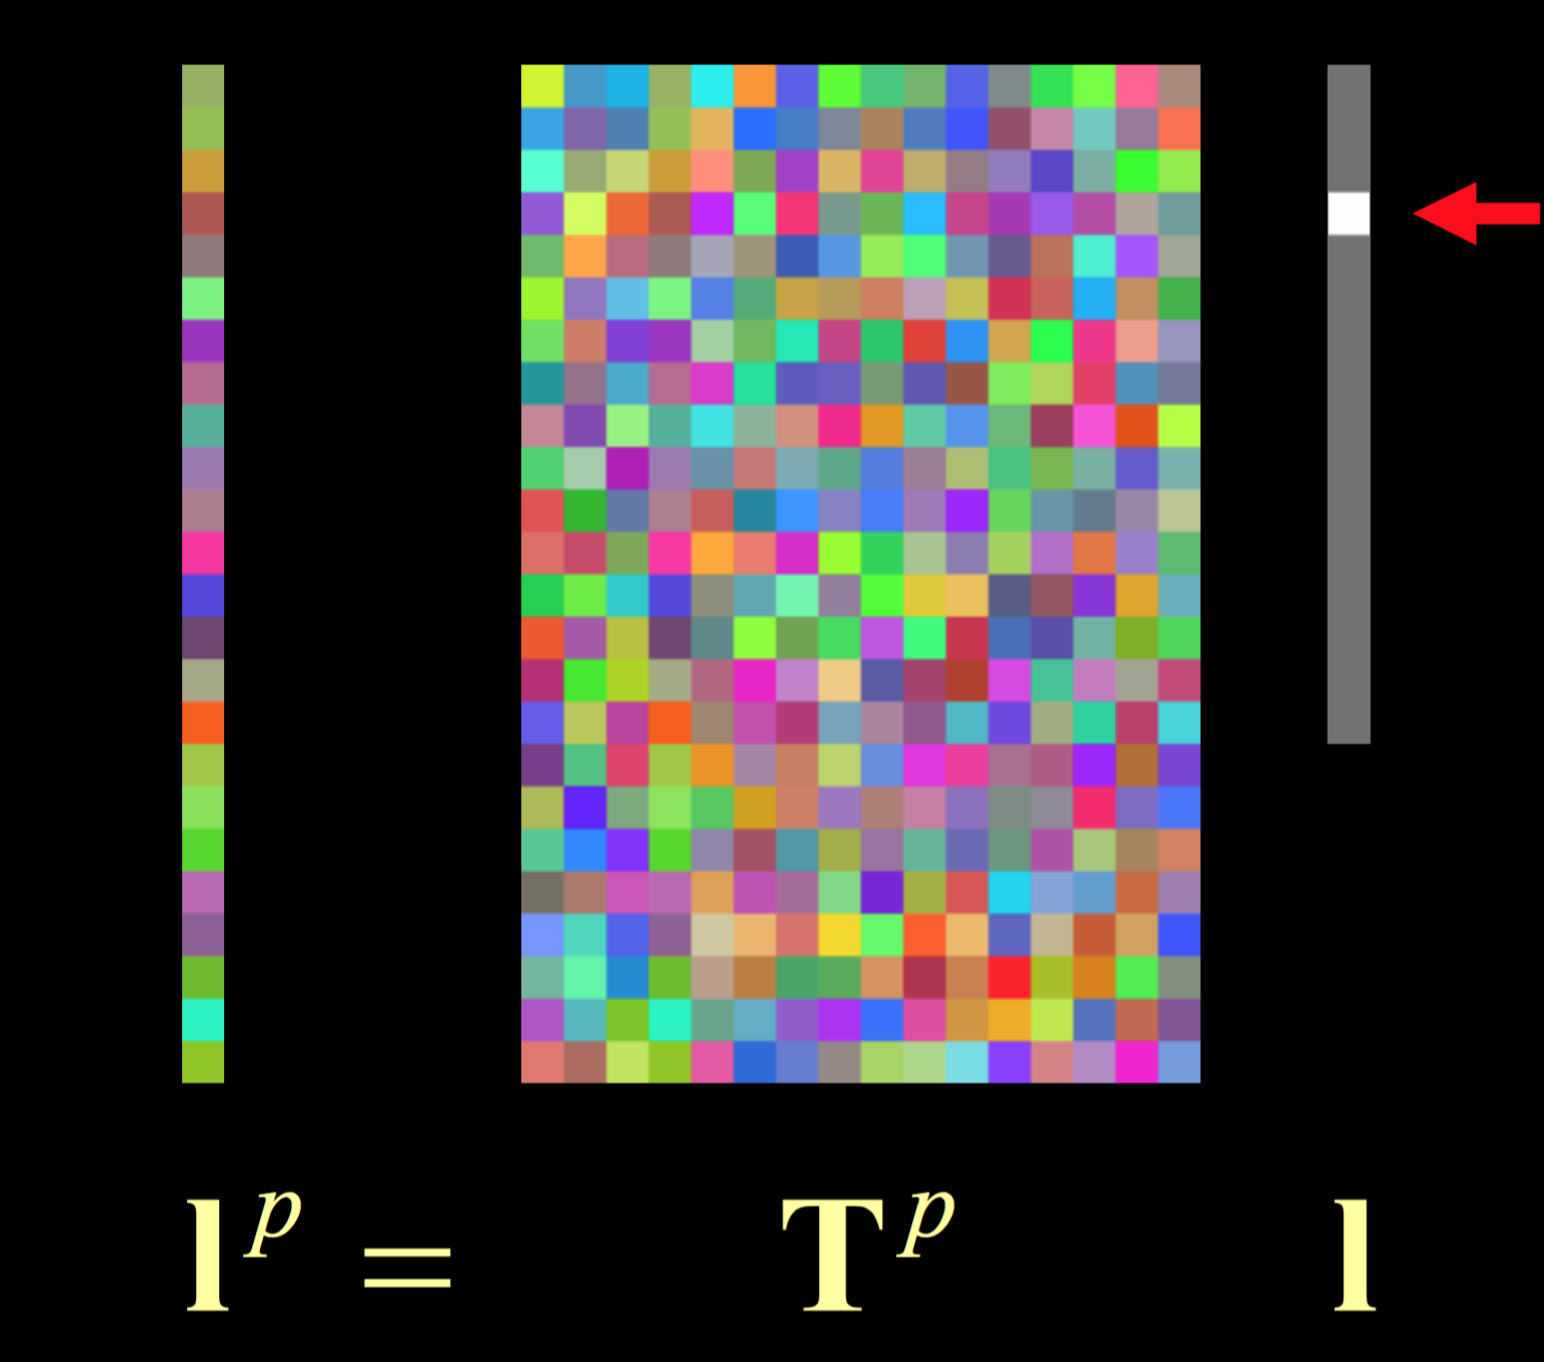
\includegraphics[width=0.5\textwidth]{figures/prt/prt-11}
	\caption{考虑入射光照仅来自单个基函数的分量,并且其光照密度为1,则经过矩阵传输的结果就是,从传输矩阵中将这个分量的序号所在的列复制出来(图片来自\cite{a:PrecomputedRadianceTransfer:TheoryandPractice})}
	\label{f:pl-matrix}
\end{figure}

由此可以得出,如果将传输入射辐射亮度看做$p$点看到的一副图像,则传输矩阵$\mathbf{T}^{p}$的第$i$列可以看做是一个基函数视觉(basis appearance),它描述的是从$p$点看到的来自环境光照的第$i$个基函数的光照。因为整个场景的环境光照是关于其各个基函数的线性组合,因此$p$点的入射光照的计算也仅仅是涉及对这些基函数视觉的线性组合,这即是矩阵和矢量相乘的原则。



\paragraph{传输矩阵的元素}
根据上面的描述,定义$L^{i}_{xfer}(p\leftarrow\omega)$为从基函数$y_i$到达点$p$的光照,这可以是直接或者经过任意次反弹的间接光照,因此传输矩阵的元素$T^{p}_{ji}$ 就表述了$L^{i}_{xfer}(p\leftarrow\omega)$的第$j$个投影系数,即:

\begin{equation}
	T^{p}_{ji}=\langle L^{i}_{xfer}(p),\hat{z}_j\rangle =\int_\Omega L^{i}_{xfer}(p\leftarrow\omega)\hat{z}_j(\omega)d\omega
\end{equation}

为了计算上式表述的矩阵的元素,我们唯一需要的就是能够计算由第$i$个光源的基函数到达$p$点的光照分布$L^{i}_{xfer}(p\leftarrow\omega)$,然后我们将该光照分布投影到基函数$\hat{z}_j$就得到了矩阵的元素$\mathbf{T}^{p}_{ji}$的值。其中这个光照分布函数$L^{i}_{xfer}(p\leftarrow\omega)$可以使用本书前面介绍的任意离线渲染的方法,例如蒙特卡洛路径追踪,光子映射算法等等。

\begin{myshaded}
	在理解上述概念时需要注意,环境光照$L_{env}$的一个基函数$y_i$的光照表述的是跟这个基函数成正比的一个光照分布,即$l_iy_i$,但是当这个光照分布到达$p$点时,它不再是跟这个阶数的基函数成正比的,而是一个全频率段的普通光照分布,即是说传输后的光照分布在各个阶数的基函数上都有投影,而矩阵的元素$\mathbf{T}_{ji}$表述的正是到第$j$个基函数的投影系数。
\end{myshaded}




\paragraph{直接光照}
现在首先来考虑最简单的直接光照,即环境光照直接到达$p$点,中间可能会被其他物体遮挡,但是光照到达$p$点之前没有经过与其他任何表面的反射,我们记到达$p$点的直接光照为$L_0$,它可以表述为环境光照与$p$点可见性函数的乘积,即:

\begin{equation}
	L_0(p\leftarrow\omega)=L_{env}(\omega)V(p,\omega)
\end{equation}

上式表述的几何图示如图\ref{f:pl-direct-light}所示,由此也可以看出,光泽表面的传输矩阵仅考虑物体表面的可见性关系。

\begin{figure}
	\sidecaption
	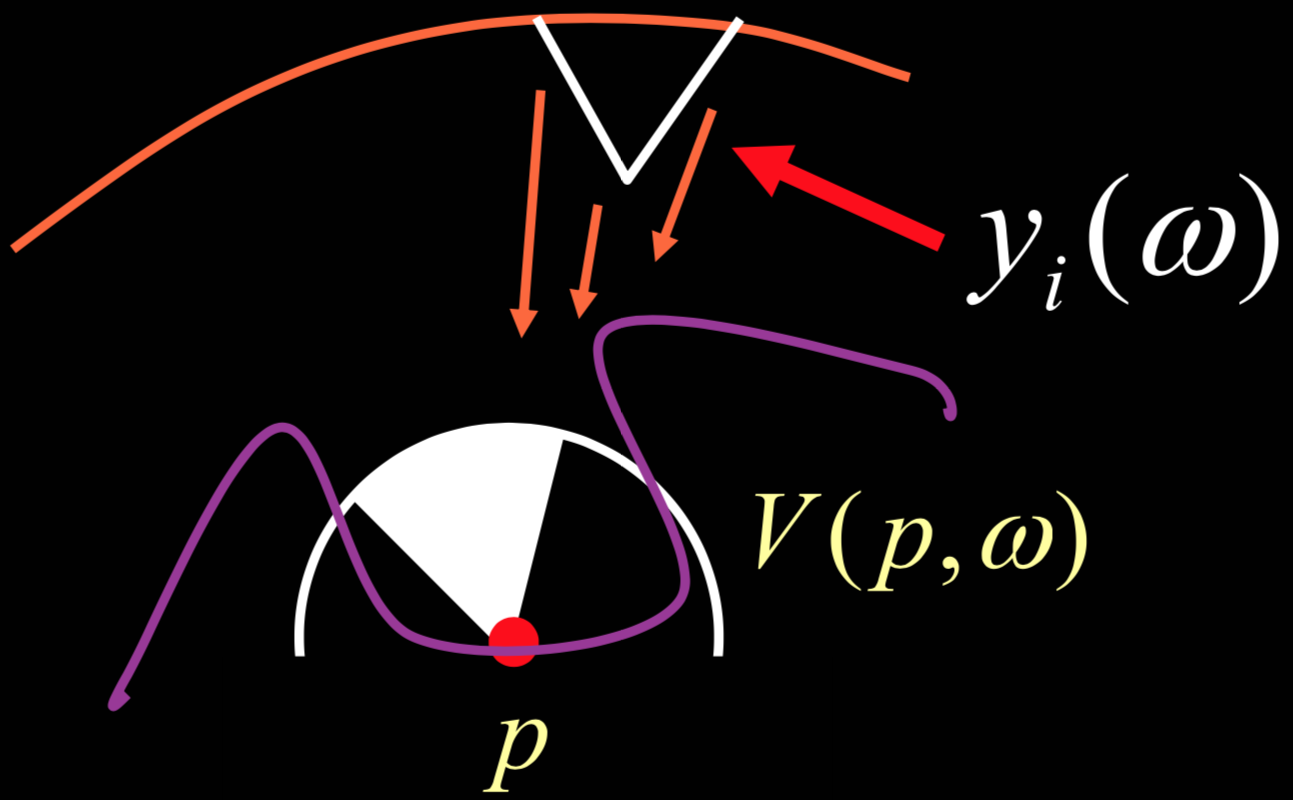
\includegraphics[width=0.45\textwidth]{figures/pl/direct-light}
	\caption{在光泽表面的PRT算法中,传输函数仅考虑可见性函数,而不是像漫反射表面一样包含BRDF分布函数。}
	\label{f:pl-direct-light}
\end{figure}

由此可知,来自基函数$y_i$并且达到$p$点的光照分布为:

\begin{equation}
	L^{i}_0(p\leftarrow\omega)=y_i(\omega)V(p,\omega)
\end{equation}

\noindent 因此得出:

\begin{equation}
\begin{aligned}
	T^{p}_{0,ji}=&\langle L^{i}_0(p\leftarrow\omega),\hat{z}_j\rangle \\
	=&\int_\Omega y_i(\omega)\hat{z}_j(\omega)V(p,\omega)d\omega
\end{aligned}
\end{equation}

我们称仅包含直接光照的传输矩阵为$\mathbf{T}^{p}_0$,如果将上式代入转移入射辐射照度的近似表达式中,即式\ref{e:pl-transfer-incident-radiance},则得到下述关于$p$点的来自直接光照的全部光照分布:

\begin{equation}
\begin{aligned}
	L(p\leftarrow\omega)\approx &\sum^{m}_{j=1}l^{p}_{j}z_j(\omega)\\
	=&\sum^{m}_{j=1}z_j(\omega)\Biggr[ \sum^{n}_{i=1}l_iT^{p}_{ji}  \Biggr]
	=\mathbf{z}(\omega)^{T}\mathbf{T}^{p}\mathbf{l}
\end{aligned}
\end{equation} 

这里第二行中间的大括号被写成矩阵的形式,它对原始环境贴图的投影系数$l_i$执行变换,将其转换成转移入射辐射照度的投影系数。



\paragraph{考虑间接光照}
接下来我们会推导出一个考虑间接光照的传输矩阵形式,它使用一种渐进式的方法,形成一个递归的公式,即给定光照的第$k$次反弹的传输矩阵,我们可以推导出第$k+1$次反弹的传输矩阵。因为已经计算出了直接光照的传输矩阵$\mathbf{T}^{p}_0$,因此我们就能够计算出任意反弹次数的传输矩阵。由于光照是线性的,因此能够考虑所有反弹的传输矩阵$\mathbf{T}^{p}$就只不过是这些单次反弹的传输矩阵$\mathbf{T}^{p}_0,\mathbf{T}^{p}_1,\cdots$的和。

为了推导出包含间接光照的传输矩阵,这里首先使用迭代形式的渲染方程,即方程两边同时包含未知的变量$L_{xfer}$,需要注意的是,与传统的渲染方程坐左边表示的是出射辐射亮度不同,这里方程的左边表示的是$p$点的入射辐射亮度:

\begin{equation}\label{e:pl-recursion}
\begin{aligned}
	L_{xfer}(p\leftarrow\omega)=&L_{env}(\omega)V(p,\omega)\\
	&+\int_{\Omega (p^{'})}L_{xfer}(p^{'}\leftarrow\omega^{'})f_r(p^{'},\omega^{'}\to -\omega)cos\theta^{'}d\omega^{'}
\end{aligned}
\end{equation}

上式说明,点$p$处的入射光照由两部分组成:

\begin{itemize}
	\item 来自于环境贴图的直接光照,其中某些方向可能会被其他物体遮挡。
	\item 来自其他物体表面反射的光照。
\end{itemize}

式\ref{e:pl-recursion}可以使用纽曼级数(Neumann series)\mathindex{纽曼级数}{Neumann series}展开,即:

\begin{equation}
	L_{k+1}(p\leftarrow\omega)=\int_{\Omega (p^{'})}L_k(p^{'}\leftarrow\omega^{'})f_r(p^{'},\omega^{'}\to -\omega)cos\theta^{'}d\omega^{'}
\end{equation}

上式说明,只要求出了第$k$次反弹的结果,则可以由此推断出第$k+1$次反弹的结果。通过递归地将方程的左边代入右边,则$p$点的转移入射辐射照度可以写为:

\begin{equation}
	L_{xfer}(p\leftarrow\omega)=L_{0}(p\leftarrow\omega)+L_{1}(p\leftarrow\omega)+L_{2}(p\leftarrow\omega)+\cdots
\end{equation}

根据前面的讨论,由于转移入射辐射照度可以被近似为球谐函数的线性组合,即:

\begin{equation}
	L_{xfer}(p\leftarrow\omega)\approx\sum^{m}_{j=1}l^{p}_jz_j(\omega)
\end{equation}

\noindent 并且上式中的系数$l^{p}_j$可以下述的积分求得:

\begin{equation}
	l_j^{p}=\int_\Omega L_{xfer}(p\leftarrow\omega)\tilde{z}_j(\omega)d\omega=:\langle L_{xfer}(p),\tilde{z}_j\rangle
\end{equation}


\noindent 因此我们可以得出$p$点处总的投影系数可以由各个反弹下的投影系数相加而得,即:

\begin{equation}\label{e:pl-all-l}
	l^{p}_j=\langle L_0(p),\tilde{z}_j\rangle+\langle L_1(p),\tilde{z}_j\rangle+\langle L_2(p),\tilde{z}_j\rangle+\cdots
\end{equation}



\paragraph{第$k+1$次反弹的传输矩阵}
首先来总结一下到目前为止我们已经掌握了那些信息,式\ref{e:pl-all-l}已经说明$p$点关于所有次反弹光照的投影系数,分别等于每一次反弹对应入射辐射亮度的投影系数之和,而对于每一次单次反弹,我们可以将它看做直接光照的形式处理,只不过这里的入射光照来自于其它表面的点而不是环境光照,这可以通过将每个表面点上一次反弹的转移入射辐射亮度值与其表面的BRDF乘积的积分计算而来。这里不再对其进行详述,请读者参考\cite{a:PrecomputedRadianceTransfer:TheoryandPractice}。




\subsubsection{出射辐射亮度}
当计算出表面每个点处的传输矩阵之后,在运行时就可以直接对环境光照执行该矩阵变换,从而得到每个像素的入射辐射亮度分布,然后我们需要将此入射光照与表面的BRDF分布函数的乘积进行积分,以计算最终观察方向的出射辐射亮度。

将一个入射光照分布映射到另一个出射辐射照度分布,这又是另一个线性操作,设$L_{out}$为出射光照分布,则有:

\begin{equation}
	L_{out}(p\to\omega_{out})=\int_{\Omega}L_{xfer}(p\leftarrow\omega_{in})f_r(p,\omega_{in}\to\omega_{out})\max(\cos \theta,0){\rm d}\omega_{in}
\end{equation}

对于上述的线性操作,我们需要一个矩阵或矢量来实现,在矩阵的情况下,入射光照分布完全被变换到一个球面上的出射光照分布,然后对给定观察方向进行取值即可;在矢量的情况下,我们可以为每个方向单独存储一个与方向有关的矢量,然后所有方向的矢量可以存储在一个类似“环境贴图”的球面纹理中,这样最后实时渲染时就用一个观察方向从这个纹理直接查询一个矢量值即可,这个矢量直接被用于入射光照的计算。这里不再对其进行详述,更详细的内容请读者参考\cite{a:PrecomputedRadianceTransfer:TheoryandPractice}。




\section{基于辐射照度的预计算}\label{sec:pl-irradiance-caching}
前面介绍的方法是对光照传输的过程进行预计算,因此光源在实时阶段是可以修改的。在接下来的两节,我们将介绍两种直接缓存光照的方法,使这些缓存的某种光照结果可以直接作用于物体表面,而不需要另外考虑光源的问题,它们就像光照计算中的一些中间结果。由此也可以推断,这两种技术无法适应光源的动态调整,除非我们可以实时动态地生成这些中间结果。

我们要介绍的第一种方法是一种基于辐射照度(irradiance)的预计算方法,辐射照度是指一个单位面积内所有入射辐射能量的总和,它是对法线方向半球空间内入射辐射亮度的积分。很显然,根据入射照度的定义,它只与漫反射表面有关,因为只有漫反射表面的出射辐射亮度才与其入射方向无关,因此各个入射方向的光照可以被加和。

对于静态场景,由于漫反射表面的光照是与观察方向无关的,因此我们可以将其辐射照度缓存起来,然后在实时渲染时将其与漫反射系数相乘的结果就可以作为表面的漫反射光照。

现代实时渲染中使用的辐射照度预计算的技术主要是光照贴图。



\subsection{光照贴图}
由于漫反射表面的颜色可以由单个RGB颜色值描述,其记载的是辐射照度值,如果光源和整个几何场景是静态的,则这个辐射照度值为一个常数,因此可以被预存起来,我们称记录辐射照度值的纹理为一个辐射照度贴图(irradiance maps)\myindex{辐射照度贴图}{irradiance maps}或光照贴图(light maps)\myindex{光照贴图}{light maps},由于光照传输是线性的,因此其它动态光源所形成的光照可以在这个辐射照度值上进行累加。光照贴图仍然是现阶段实时渲染中漫反射间接光照的主流解决方案\cite{m:LightmappingQuickstart,m:LightmassGlobalIllumination,a:PrecomputedLightinginCallofDuty},它最早被用于\cite{a:QuakesLightingModel:SurfaceCaching}中,光照贴图的概念如图\ref{f:pl-lightmap}所示。

\begin{figure}
\begin{fullwidth}
	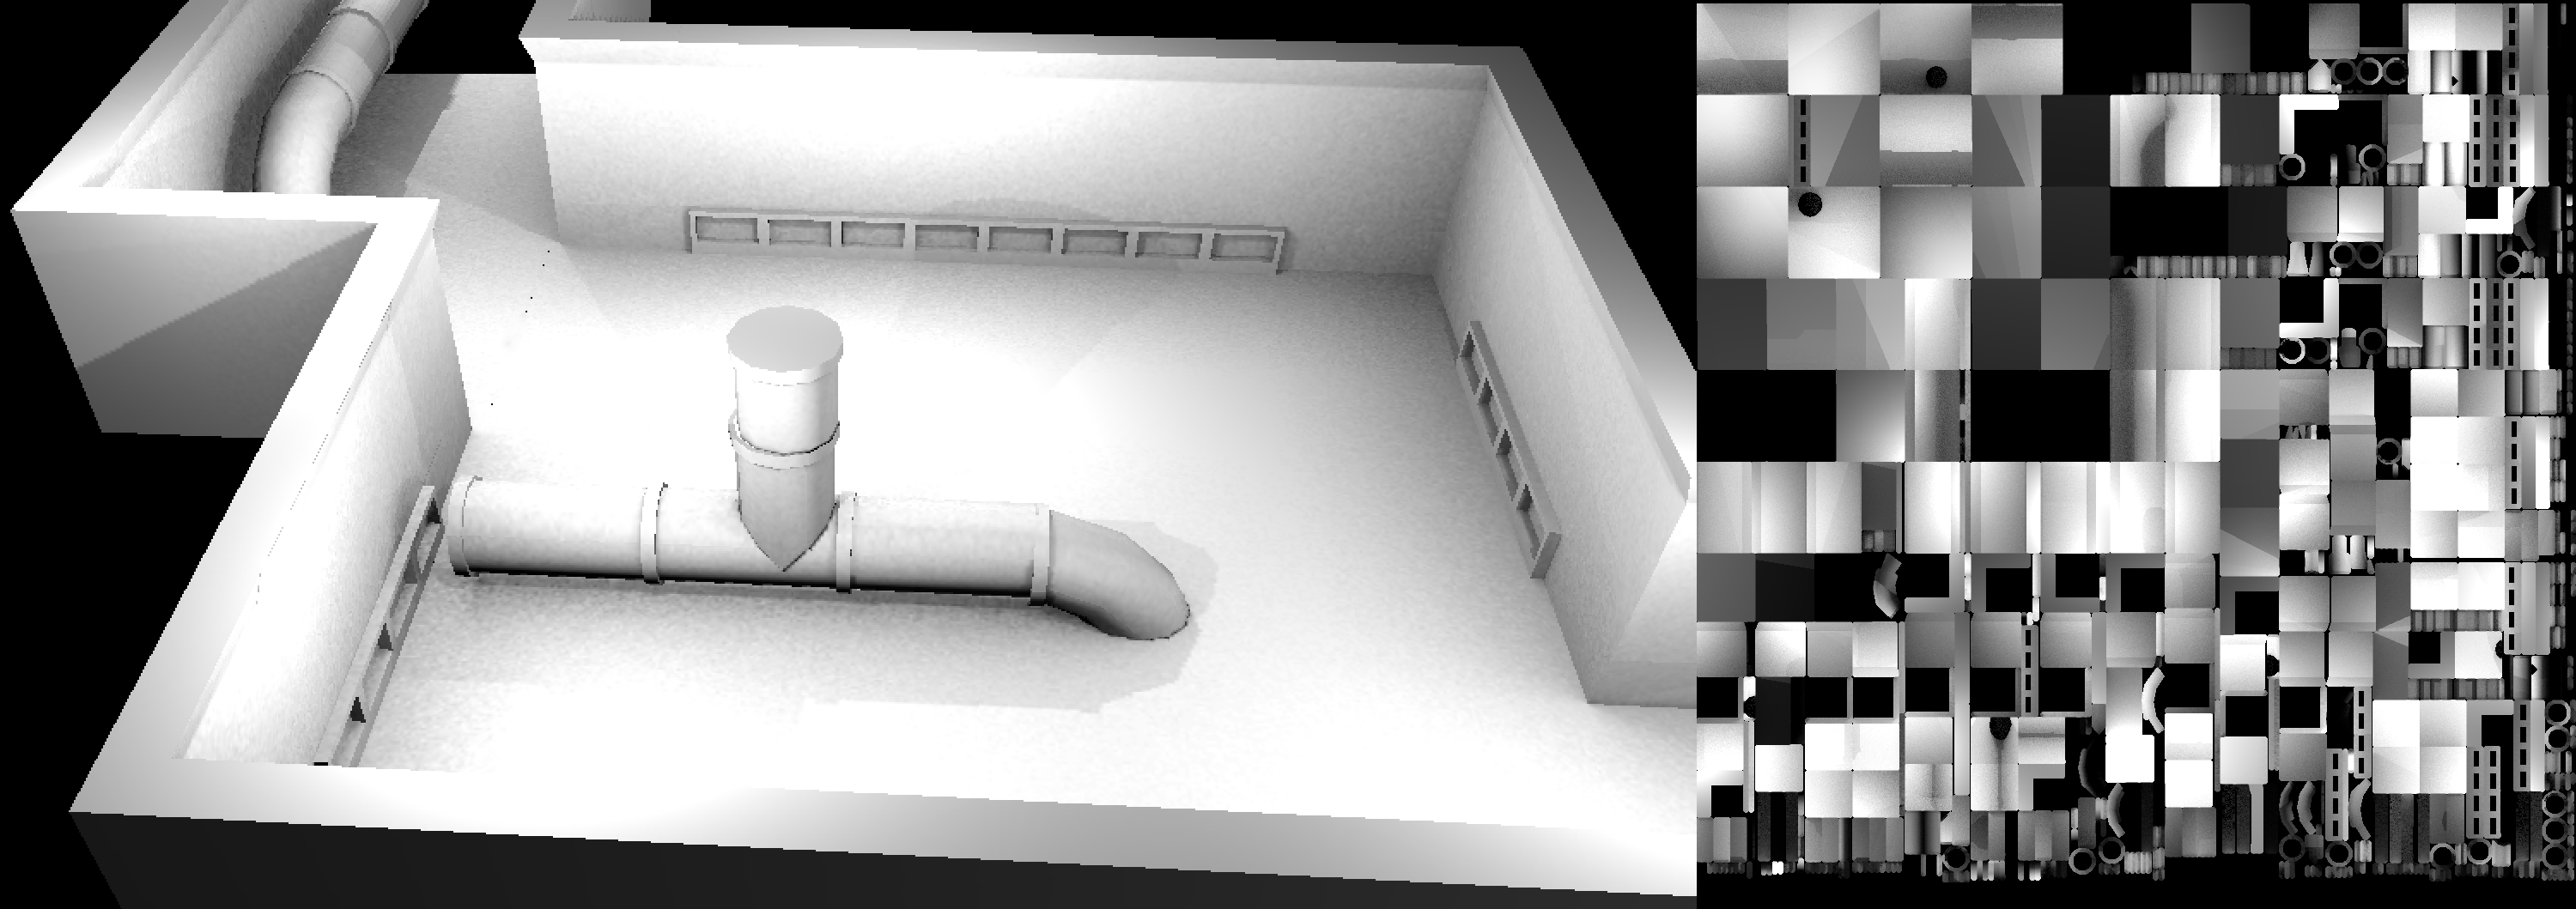
\includegraphics[width=\thewidth]{figures/pl/pl-lightmap}
	\caption{一个简单的场景(左)及其光照贴图(右),由此可以看出光照贴图的分辨率很低,因此它通常仅用来存储间接光照(图片来自Wikipedia)}
	\label{f:pl-lightmap}
\end{fullwidth}
\end{figure}

在像素着色器中,每个像素都需要读取光照贴图中的一个辐射照度值,我们已经说明它是一个常数颜色值;而另一方面,漫反射表面的每个像素还存储了一个漫反射系数值,它也是一个常数值。直观上思考,我们希望将这两个值预乘起来,形成一个直接的出射辐射亮度值,这样便可以使用一个单独的纹理来同时存储漫反射颜色和光照贴图中的数据,然而有几个原因使得我们通常不会这么做。

首先,漫反射颜色除了用于静态的光照计算,这里即是光照贴图中的这部分光照,它还可能会被用于动态光源的光照计算,例如下一节介绍的环境探针,所以表面的漫反射颜色是必须单独存储的,除非场景完全由静态光源组成。

其次,对所有表面存储每像素的辐射照度值会占据很大的存储空间,所以在实践中光照贴图的分辨率会远远小于漫反射颜色的分辨率,因此它们必须单独存储。由于这种较低的分辨率特征,它不能很好地近似高频的直接光照分布,光照贴图通常只存储间接光照,因为表面间接光照分布会更加平滑,而直接光照仍然交由光栅化处理。也正是因为光照贴图的分辨率很低,所以我们通常不需要对每个物体表面单独存储一个纹理,而是对整个或部分场景存储一个光照贴图,如图\ref{f:pl-lightmap}所示。



光照贴图本身只是存储辐射照度值的一个数据结构,它并不包含产生辐射照度值的方法。由于光照贴图仅针对漫反射表面,所以本书前面介绍的两种辐射度设置方法(即辐射度方法和即时辐射度方法)都可以用于生产光照贴图的辐射照度颜色值,当然原始的光线追踪方法也可以用于生成光照贴图,只是这种方法的收敛速度回非常慢。除此之外,另一种常用于生成光照贴图的技术是辐射照度缓存,由于其并不涉及太多复杂算法,这里并不对其进行详细介绍,感兴趣的读者可以参考\cite{b:pbrt2}第15.5节的内容。

\begin{myshaded}
	这里对辐射照度缓存做一个简要介绍,辐射照度缓存(irradiance caching)\myindex{辐射照度缓存}{irradiance caching}是一种有偏估计(biased estimator)\myindex{有偏估计}{biased estimator},由于无偏方法需要依赖于大量的相互之间独立的随机样本,才能生成噪点比较低的图像,因此为了提高计算效率,有偏的方法通常通过重用一些中间或部分结果,来避免使用距离的随机样本,这种重用通常涉及对已有某种中间或部分结果的线性插值,所以这就依赖于某个量具有比较平滑的分布。在渲染算法中,只有漫反射表面的分布具备这种特征,因为漫反射与观察方向无关,漫反射表面的出射辐射亮度相当于混合了所有方向的入射光照,因此它才能够具备这种平滑分布的特征。

	所以离线渲染中两大(注意,即时辐射度也是一种有偏方法,但是它的有偏性并不来源于对已有样本的线性插值,因为已有的样本只是作为直接光源被使用,即时辐射度的有偏性来源于对被积函数取值的限定,这方面的内容可以参见第\ref{chp:ir}章第\ref{sec:bias-compensation}节关于其有偏性的描述。)有偏估计都是和漫反射有关的,即光子映射和这里的辐射照度缓存,光子映射通过对分布于漫反射表面的辐射能量样本进行回归拟合,以期找出漫反射表面各个位置处的辐射能量分布,使得任意的摄像机子路径都可以与某些光源子路径“相连”;而本节介绍的辐射照度缓存的主要思路,则是对表面的辐射照度进行稀疏采样,然后任意其它位置的辐射照度则通过对这些稀疏样本的线性插值计算而来。
\end{myshaded}





\subsection{辐射照度体积}\label{sec:pl-irradiance-volume}
上面介绍的光照贴图只能计算静态物体的间接漫反射光照,但是,场景中的一些动态物体(如角色)同样也需要一种方法来计算间接光照;另一方面,由于光照贴图直接将辐射照度值存储于表面上,因此它使用非常低的分辨率以节省存储开支,这使得它无法应对一些具有非常精细局部结构的表面,例如那些法线分布频率非常高的表面。

为了解决上述关于光照贴图的问题,\cite{a:TheIrradianceVolume}首先提出了称为辐射照度体积的概念,该技术随机被运用在离线的电影工业当中,例如\cite{a:RenderinginCars2},随后\cite{a:IrradianceVolumesforGames}将其引入到实时渲染当中,如今,主流的游戏引擎基本上都在使用该种技术,例如\cite{a:VolumetricGlobalIlluminationAtTreyarch,m:VolumetricLightmaps,m:LightProbes}等。

与光照贴图不一样,辐射照度体积(irradiance volume)\myindex{辐射照度体积}{irradiance volume}将辐射照度值稀疏地存储在场景中的空白位置处,例如图\ref{f:pl-irradiance-volume}(a)所示,然后场景中位于辐射照度体积内任意一点的辐射照度值,可以通过对附近的样本执行某种插值计算而来,我们将在后面介绍两种常用的插值方法。辐射照度体积在\cite{m:VolumetricLightmaps}中又被称为体积光照贴图(volumetric lightmaps)\myindex{体积光照贴图}{volumetric lightmaps},在\cite{m:LightProbes}中则被称为光照探针(light probes)\myindex{光照探针}{light probes},为了便于更好地对比概念,本书后面将称使用体积光照贴图这个称谓,并称空间中的每个样本为体积光照样本。

\begin{figure}
	\begin{subfigure}[b]{0.5265\textwidth}
		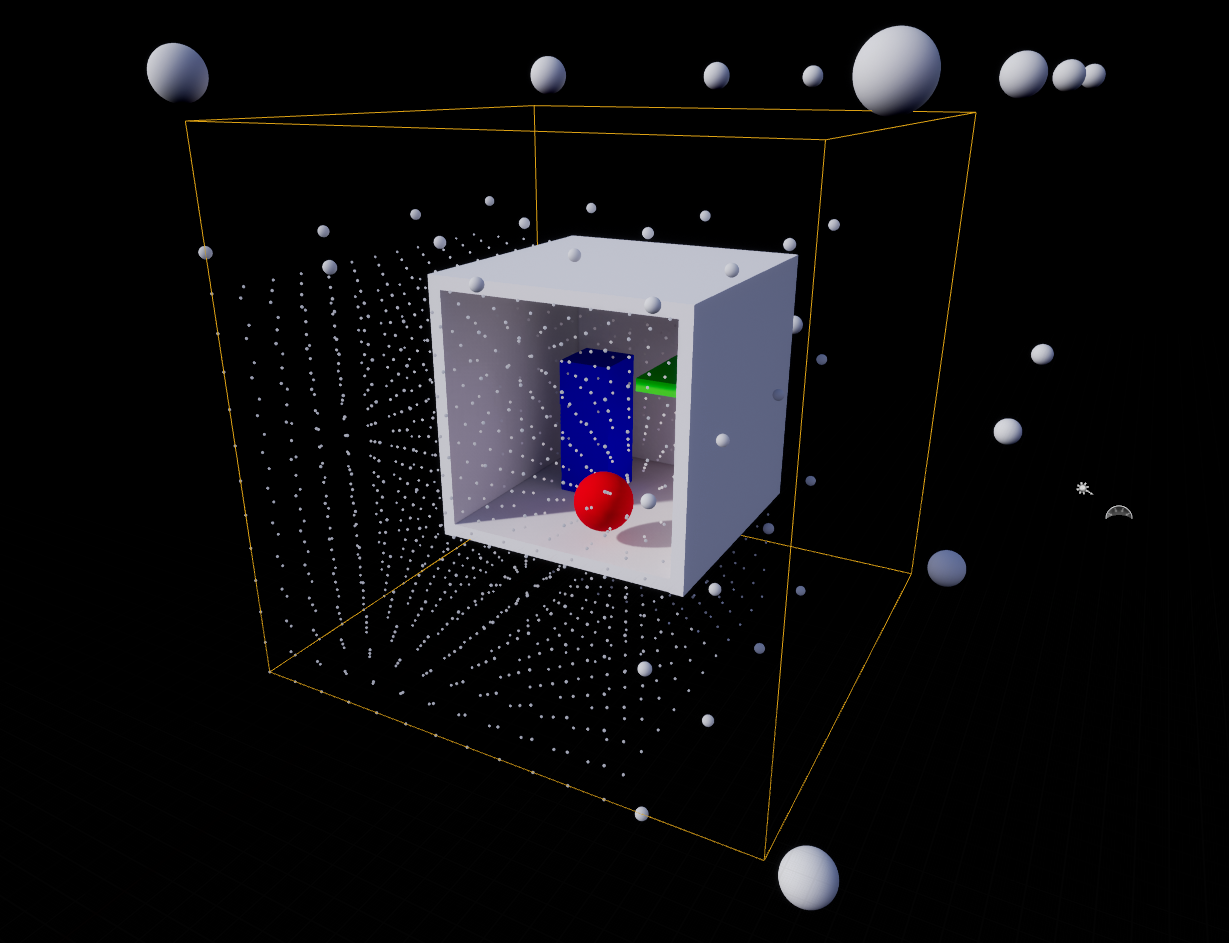
\includegraphics[width=\textwidth]{figures/pl/VLM_Placement}
		\caption{}
	\end{subfigure}
	\begin{subfigure}[b]{0.4735\textwidth}
		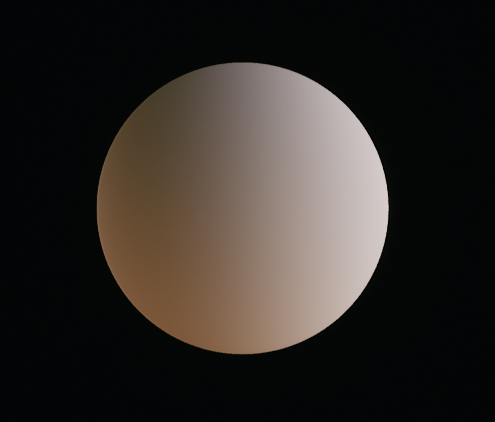
\includegraphics[width=\textwidth]{figures/pl/VolumeLightmap}
			\caption{}
	\end{subfigure}
	\caption{辐射照度体积把辐射照度值稀疏地存储在空白空间处(a),然后通过插值来计算体积内任意位置处的辐射照度值,由于空白空间位置并不存储某个法线方向,因此辐射照度体积中的样本存储的是一个辐射照度的方向分布函数(b),在Unreal Engine 4中是一个3阶的球谐函数投影,其中每个方向存储一个辐射照度值(图片来自Unreal Engine 4官方文档)}
	\label{f:pl-irradiance-volume}
\end{figure}

在光照贴图中,给定表面及其法线方向,表面上每个位置处的辐射照度就是一个标量值,然而将这个概念推广到空白空间却会发生变化,因为空白空间中的位置并不包含任何法线方向,而我们要计算的表面位置的法线方向可能是任意的。因此,为了满足这个需求,体积光照贴图中每个样本中存储的就不能是(针对某个法线方向的)单个辐射照度值,而是应该所有的法线方向,这就形成了一个辐射照度方向分布函数,如图\ref{f:pl-irradiance-volume}(b)所示。由于辐射照度分布是一个方向函数,因此在它可以被存储在一个立方体贴图或类似的方向贴图中,但是这会占用较多的存储空间,因为场景中可能存在大量的体积光照样本。由于辐射照度函数值是低频的,因此我们也可以使用前面介绍的低阶球谐函数来近似这个方向分布函数,例如Unreal Engine 4中使用3阶球谐函数来近似一个体积光照样本,这样每个体积光照样本就只需要存储少数几个系数值即可。

为了生成体积光照样本,在预处理阶段\footnote{需要注意的时,体积环境贴图也可以实时生成,只要相应的方法能够满足实时需求,例如在Enlighten中,由于整个漫反射的传输过程被转换为针对一些细分曲面的矩阵变换,所以它能够较快地实时生成光照探针,因此在Unity中光照探针也能够捕捉动态光源的光照。},我们首先将摄像机置于样本位置处,然后渲染一个标准的环境贴图,由于环境贴图记录的是反射光照,因此我们需要使用余弦函数作为核函数对环境贴图执行过滤操作,以将其中的入射辐射亮度值转换为辐射照度值(可以参考本章前面的内容),这得到一个辐射照度贴图(irradiance map)\myindex{辐射照度贴图}{irradiance map},最后我们将该立方体贴图投影到球谐函数表述上。

读者会发现,上述的整个过程是和前面的环境辐射照度贴图是类似的,其唯一的区别是,环境辐射照度贴图是记录的是整个场景,它适用于反射来自较远位置的间接光照,例如来自天空环境的间接光照;而体积光照样本记录的只是局部位置的环境光照,例如室内或者一个很小区域内的环境光照,因为当一个角色移动到室内时,其显然不能再接受来自天空的环境,而是应该反射室内的局部环境,所以我们需要注意这种全局和局部的区别,也正是因此,局部的体积光照样本通常会被限制于一定的局部范围,例如图\ref{f:pl-irradiance-volume}(a)中的立方体包围盒区域,这在Unreal Engine中称为一个重要性体积(importance volume)\myindex{重要性体积}{importance volume}。



\subsubsection{插值计算}
在全局的环境照度贴图,只需要使用一个像素的法线方向即可以查询到来自环境的间接光照,而对于局部的体积光照样本,它们是与位置有关的,因此我们需要对来自着色像素附近的体积光照样本的光照值进行插值计算,因此对于每个着色像素,我们需要决定哪些体积光照样本被用于插值计算,以及每个被选择的体积光照样本被赋予多少权重。

对体积光照样本进行插值计算的方式主要取决于体积样本的数据结构,例如体积光照样本可能采样八叉树结构,规则的网格结果或者其它细分结构,我们将在下一节介绍常用的几种细分结构。对于给定某种结构,体积样本插值算法首先会找到一些最近邻样本形成一个包围着色像素的体积结构,然后在这些样本之间进行插值计算。

\begin{myshaded}
	这里可能会产生一点疑问:着色像素一定会位于某几个体积光照样本包围的体积之内吗?这样的说法通常是正确的,尽管体积光照样本通常是位于空白空间,如图\ref{f:pl-irradiance-volume}(a)所示,但是使用体积光照贴图进行间接光照计算的通常是动态物体,相对于静态场景,这些动态物体其实也是位于空白空间当中,而且体积光照样本的放置通常会覆盖到动态物体可能会占据的范围,所以这里可以假设着色像素始终是位于体积光照样本构成的某个体积之内。
	
	退一步讲,即使着色像素不是位于体积光照样本体积之内,而是位于某三个或更少体积光照样本的附近,这个时候仍然是可以进行插值计算的,因为插值方法的核心是怎样分配给各个样本一个权重值,只要最后参与插值计算的各个样本的权重值能够被归一化即可。例如由于光照贴图的分别率极低,其间接光照不容易很好的处理比较精细的表面,所以除了针对动态物体,在\cite{a:PrecomputedLightinginCallofDuty}中同时也会使用体积光照贴图来对具有精细结构或者光照质量要求比较高的表面进行间接光照的计算,因为体积光照贴图可以逐像素计算,它能够使用表面的精细结构,例如表面具有高频的法线分布函数。
\end{myshaded}

最简单也是最常用的体积光照样本数据结构是规则网格(regular grid)结构,在这种结构中,样本在各个坐标轴方向上以相同的间距均匀分布,在这种结构中,任意一个待着色计算的像素位置始终位于由相邻的8个体积光照样本构成的正立方体中,因此可以使用三线性插值(trilinear interpolation)\myindex{三线性插值}{trilinear interpolation}来计算该像素的辐射照度值,如图\ref{f:pl-trilinear-interpolation}所示。

\begin{figure}
	\sidecaption
	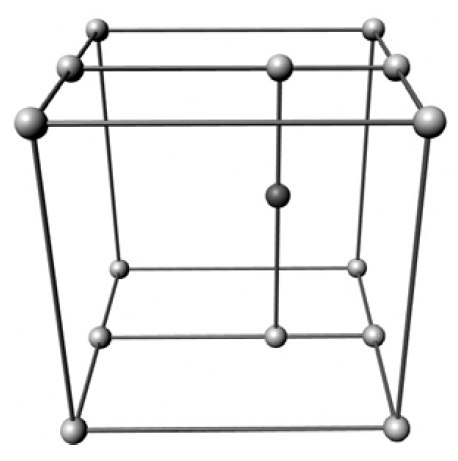
\includegraphics[width=0.3\textwidth]{figures/pl/trilinear-interpolation}
	\caption{对规则网格结构的体积光照贴图使用三线性插值计算着色像素的辐射照度值}
	\label{f:pl-trilinear-interpolation}
\end{figure}

尽管规则网格结构的生成和插值计算都比较简单,但是它用在体积光照贴图中却存在一些问题,首先是规则网格结构容易导致欠采样(undersampling)和过采样(oversampling),前者存在于那些需要使用更高采样密度的区域,而后者存在于那些可以使用更稀疏采样的区域。针对此一些改进方法是使用多种分辨率的规则网格,例如在Unreal Engine 4中,靠近物体表面的规则网格具有更高的采样密度,而随着距离表面的距离增加,其规则网格的分辨率会降低,如图\ref{f:pl-VLMDensity}所示。尽管这种多分辨率的结构能够更好地适应采样密度的需求,但是这种分辨率之间的跳跃并不能很好地近似实际的光照变化情况,我们将在下一节介绍一些更具适应性的细分方法。

\begin{figure}
\begin{fullwidth}
	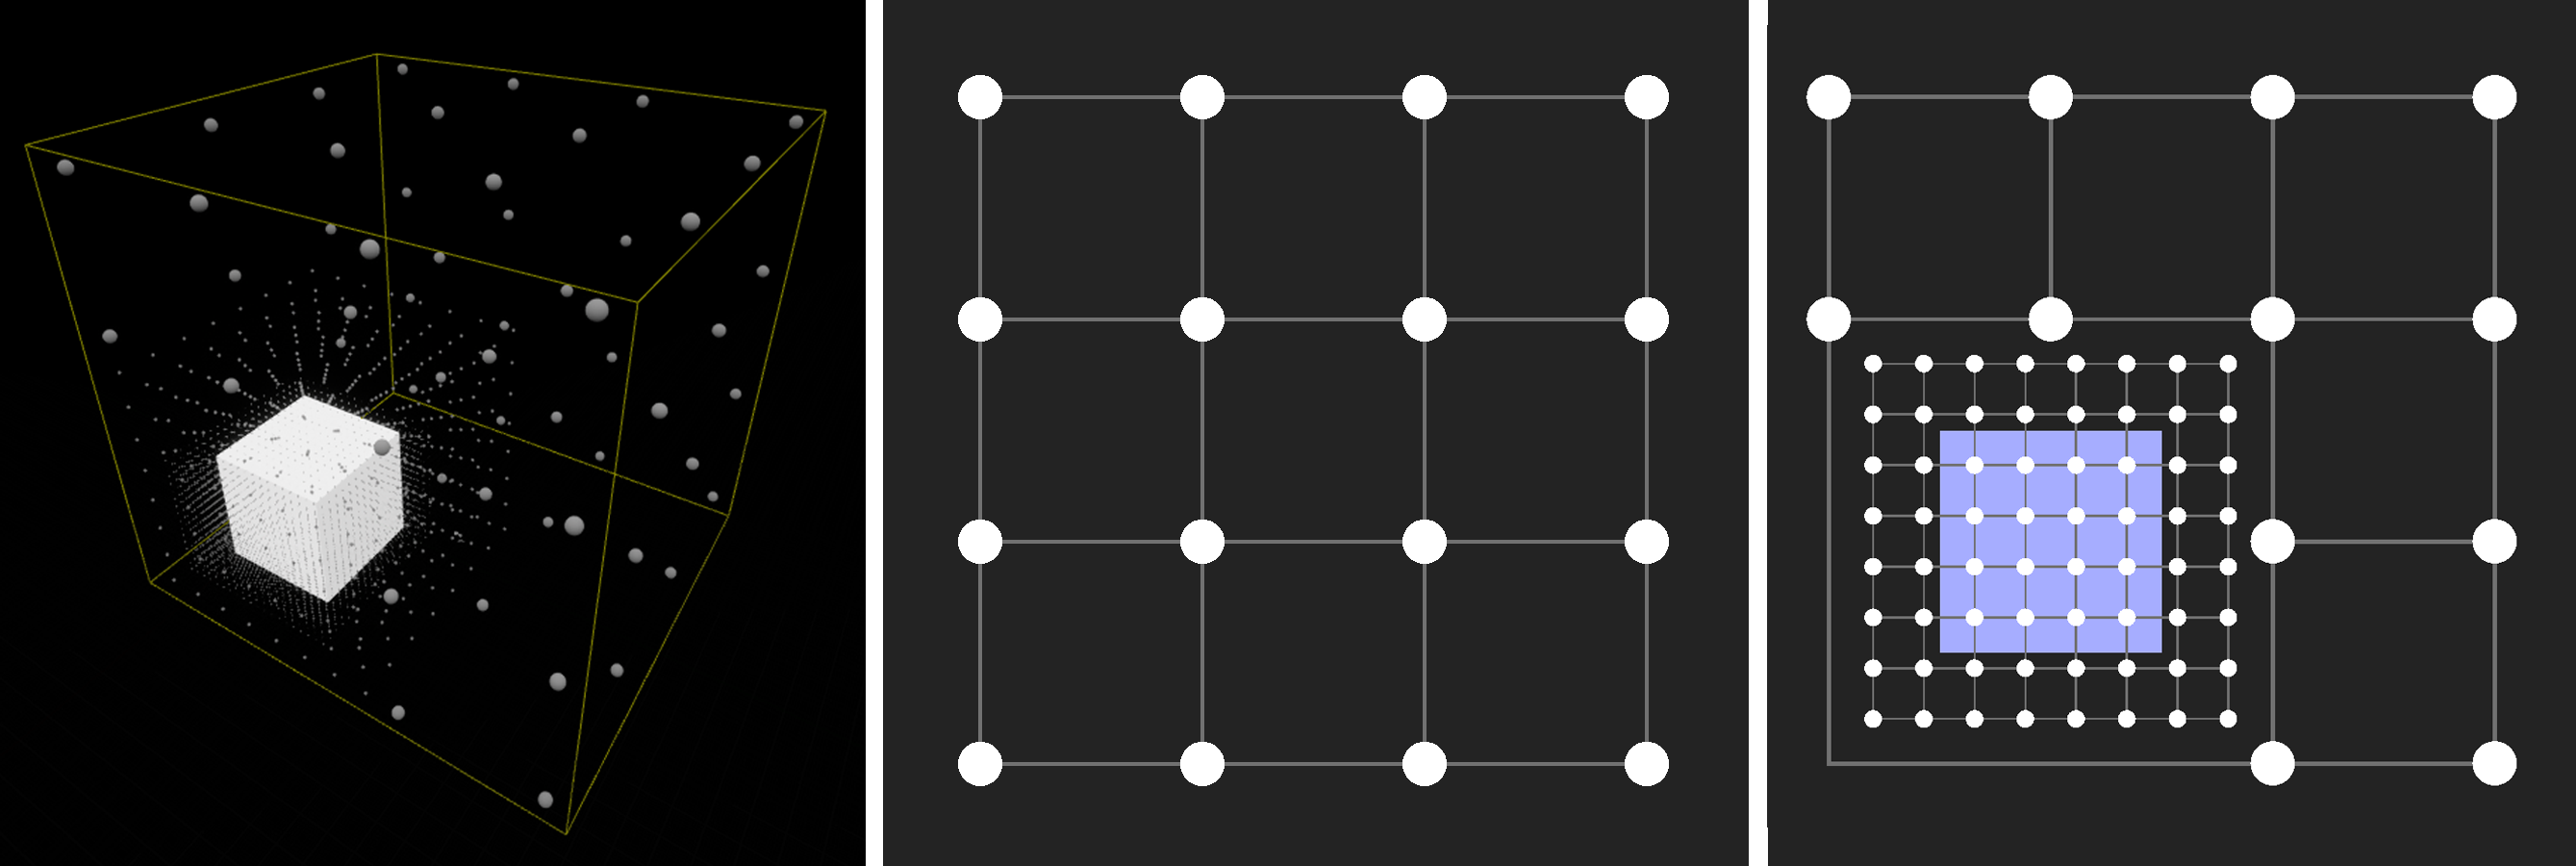
\includegraphics[width=\thewidth]{figures/pl/VLMDensity}
	\caption{从左到右:每个物体包含一个重要性体积,该体积用于存储规则结构的体积光照样本,围绕几何表面的区域拥有更高的采样密度;一个分辨率为$4\times 4\times 4$的网格侧面;在几何体附近的区域拥有更高的采样密度(图片来自Unreal Engine 4官方文档)}
	\label{f:pl-VLMDensity}
\end{fullwidth}
\end{figure}

规则网格结构的另一个是涉及到可见性的问题\cite{a:VolumetricGlobalIlluminationAtTreyarch},由于体积光照样本是均匀分布的,它在生成的时候通常并不考虑实际的几何表面分布,这就会导致一些体积光照样本出现在物体内部或者场景之外的区域,而这些样本并不包含颜色值或者包含错误的颜色值,如果一些运动物体进入到这些包含错误样本的区域,就会出现错误的光照结果。例如图\ref{f:pl-cars2}展示了轨道外部一些非法的样本,当汽车靠近通道的墙面时,其间接光照就可能与墙外错误的光照进行混合。\cite{a:RenderinginCars2}使用了一种特殊而简单的方法来处理这个问题,即当样本位于非法区域时,直接对其复制附近合法的体积光照样本值。另一些方法则尝试计算着色像素和体积光照样本之间的可见性,我们将在后面介绍一些这样的方法。

\begin{figure}
	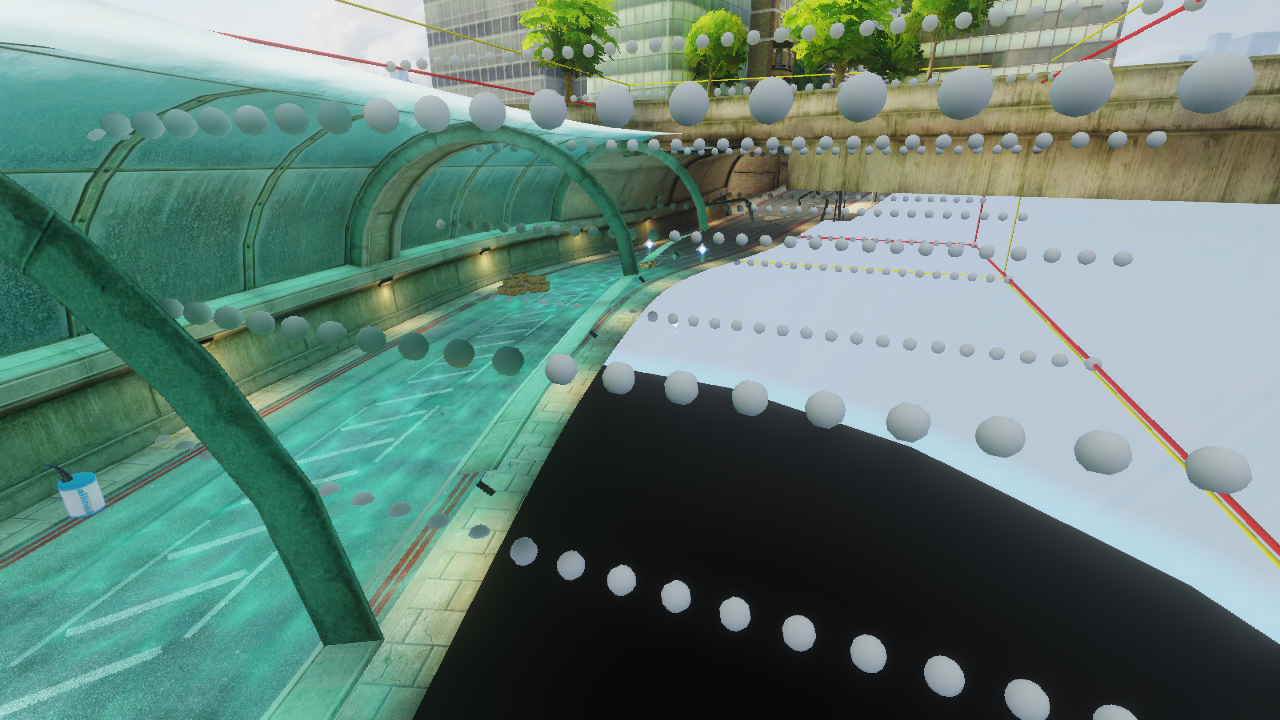
\includegraphics[width=\textwidth]{figures/pl/cars2}
	\caption{使用规则结构的体积光照样本,则可能导致一些样本出现于非法的区域,例如那些超出场景之外区域,即本图中赛车通道之外(右边)的那些区域(图片来自\cite{a:RenderinginCars2})}
	\label{f:pl-cars2}
\end{figure}




\paragraph{四面体插值}
为了避免体积光照样本出现于非法区域,我们希望样本能够位于任意位置,这种情况下就需要能够对任意分布的体积光照样本执行插值计算的能力,同时可以在任意位置摆放的体积光照样本也使得我们可以使用更好的适应性细分方法,这将在下一节讨论。

针对此目标,\cite{a:Lightprobeinterpolationusingtetrahedraltessellations}提出了一种四面体插值方法,在该方法中,体积光照样本被按照三角化的方式构建,其中每个样本可能出现在任意位置,然后一个给定的着色像素则会位于某个由4个相邻样本构成的四面体中,最后像素的颜色值由这四个样本插值计算而来,其中样本位置的三角化细分,以及搜索着色像素所在四面体的顶点样本位置将在下一节介绍。

给定一个四面体,我们可以使用重心坐标系(barycentric coordinate system)\mathindex{使用重心坐标系}{barycentric coordinate system}来将四面体内的任意顶点的位置表述成四面体四个顶点位置的线性组合,如图\ref{f:pl-barycentric-coordinates}所示,而这个线性组合的各个系数,就可以作为每个顶点样本的权重值,这跟二维的三角形插值是类似的方法,我们称之为四面体插值。

\begin{figure}
	\sidecaption
	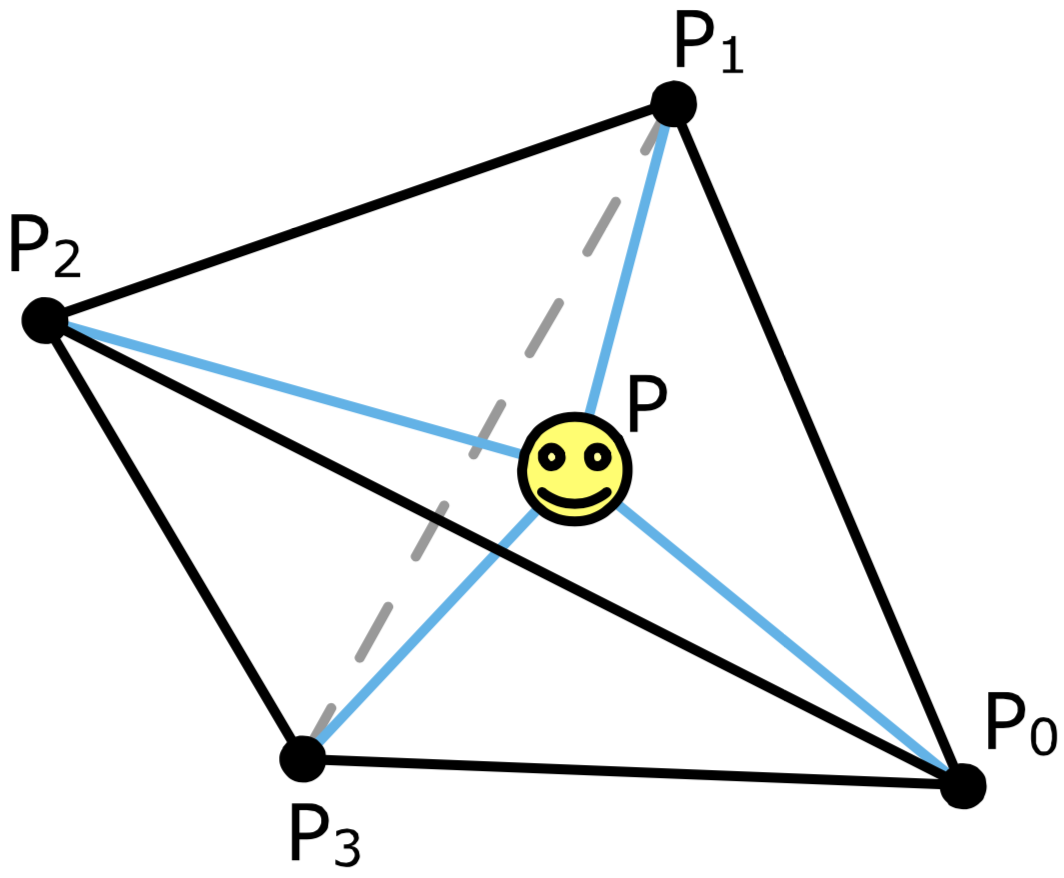
\includegraphics[width=0.4\textwidth]{figures/pl/barycentric-coordinates}
	\caption{一个四面体,在重心坐标系下,四面体内的任意一点$\mathbf{p}$的位置可以表述为四个顶点$\mathbf{p}_0,\mathbf{p}_1,\mathbf{p}_2$和$\mathbf{p}_3$的线性组合}
	\label{f:pl-barycentric-coordinates}
\end{figure}

对于一个四面体,设重心坐标系为$(\lambda_0, \lambda_1,\lambda_2,\lambda_3)$,它表示的是一个点在朝着各个顶点的方向上距离四面体重心的距离,其中重心的坐标为$(0,0,0,0)$,在规则化的重心坐标系下,满足$\lambda_0+ \lambda_1+\lambda_2+\lambda_3=1$,因此四个顶点在重心坐标系下的坐标值分别为$(1,0,0,0),(0,1,0,0),(0,0,1,0)$和$(0,0,0,1)$。

如图\ref{f:pl-barycentric-coordinates}所示,设四面体四个顶点在笛卡尔坐标系下的坐标分别为:$\mathbf{p}_0=(x_0,y_0,z_0),\mathbf{p}_1=(x_1,y_1,z_1),\mathbf{p}_2=(x_2,y_2,z_2),\mathbf{p}_3=(x_3,y_3,z_3)$,点$\mathbf{p}=(x,y,z)$位于该四面体内部,顶点$\mathbf{p}$的重心坐标值可以由下式求得:

\begin{equation}
\begin{aligned}
	\begin{bmatrix}
		\lambda_0 \\ \lambda_1 \\\lambda_2
	\end{bmatrix}=&\mathbf{T}^{-1}\bigg[ \mathbf{p}-\mathbf{p}_3\bigg]\\
	\lambda_3=&1-\lambda_0-\lambda_1-\lambda_2
\end{aligned}
\end{equation}

\noindent 这里$\mathbf{T}$表示一个由笛卡尔坐标系向重心坐标系的变换矩阵:

\begin{equation}
	\begin{bmatrix}
		x_0-x_3 & x_1-x_3 & x_2-x_3 \\
		y_0-y_3 & y_1-y_3 & y_2-y_3 \\
		z_0-z_3 & z_1-z_0 & z_2-z_3
	\end{bmatrix}
\end{equation}

由此可以看出,坐标变换矩阵$\mathbf{T}$与着色点坐标$\mathbf{p}$无关,我们可以简单地通过笛卡尔坐标系的坐标值求出其在重心坐标系下的坐标值,这些坐标值反映了四面体内各个顶点相对于重心的位置关系,因此可以被用来作为插值计算的权重系数。

重心坐标系不仅能够用于计算某个点的重心坐标值,还能够用于判断一个点是否位于四面体内部,下一节将使用这种方法来辅助对体积光照样本的位置执行细分操作。




\subsubsection{适应性细分}
从上面的内容可以看出,四面体插值比三线性插值要复杂得多,但是它的好处是可以在场景中任意放置体积光照样本的位置,因此我们能够根据场景的光照分布来调整体积光照样本的密度,从而形成更好地适应性细分结构。尽管一些其它的数据结构(例如八叉树结构)也能很好地调整体积样本的采样密度,但是这里我们只讨论\cite{a:Lightprobeinterpolationusingtetrahedraltessellations}介绍的四面体细分方法。

那么怎么生成体积光照样本的四面体网格结构呢?我们的主要目标是要能够随意放置体积光照样本的位置,有了这种能力,首先算法会标记出一些关键的位置以防止样本落入物体内部或者其它非法区域,如图\ref{f:pl-key-points}中墙面附近的关键位置,这样能够保证空白空间的位置始终位于4个合法的样本构成的四面体内部,因此避免了对体积光照样本和着色像素之间的可见性判断;其次,除了这些具有非连续性的关键位置,其它一些光照场分布变化比较大的区域也应该放置更多的样本,这可以通过在预计算阶段计算空白空间光照场的梯度来实现,这种梯度考量的结果是样本的密度能够与光照场的分布相适应。

\begin{figure}
	\sidecaption
	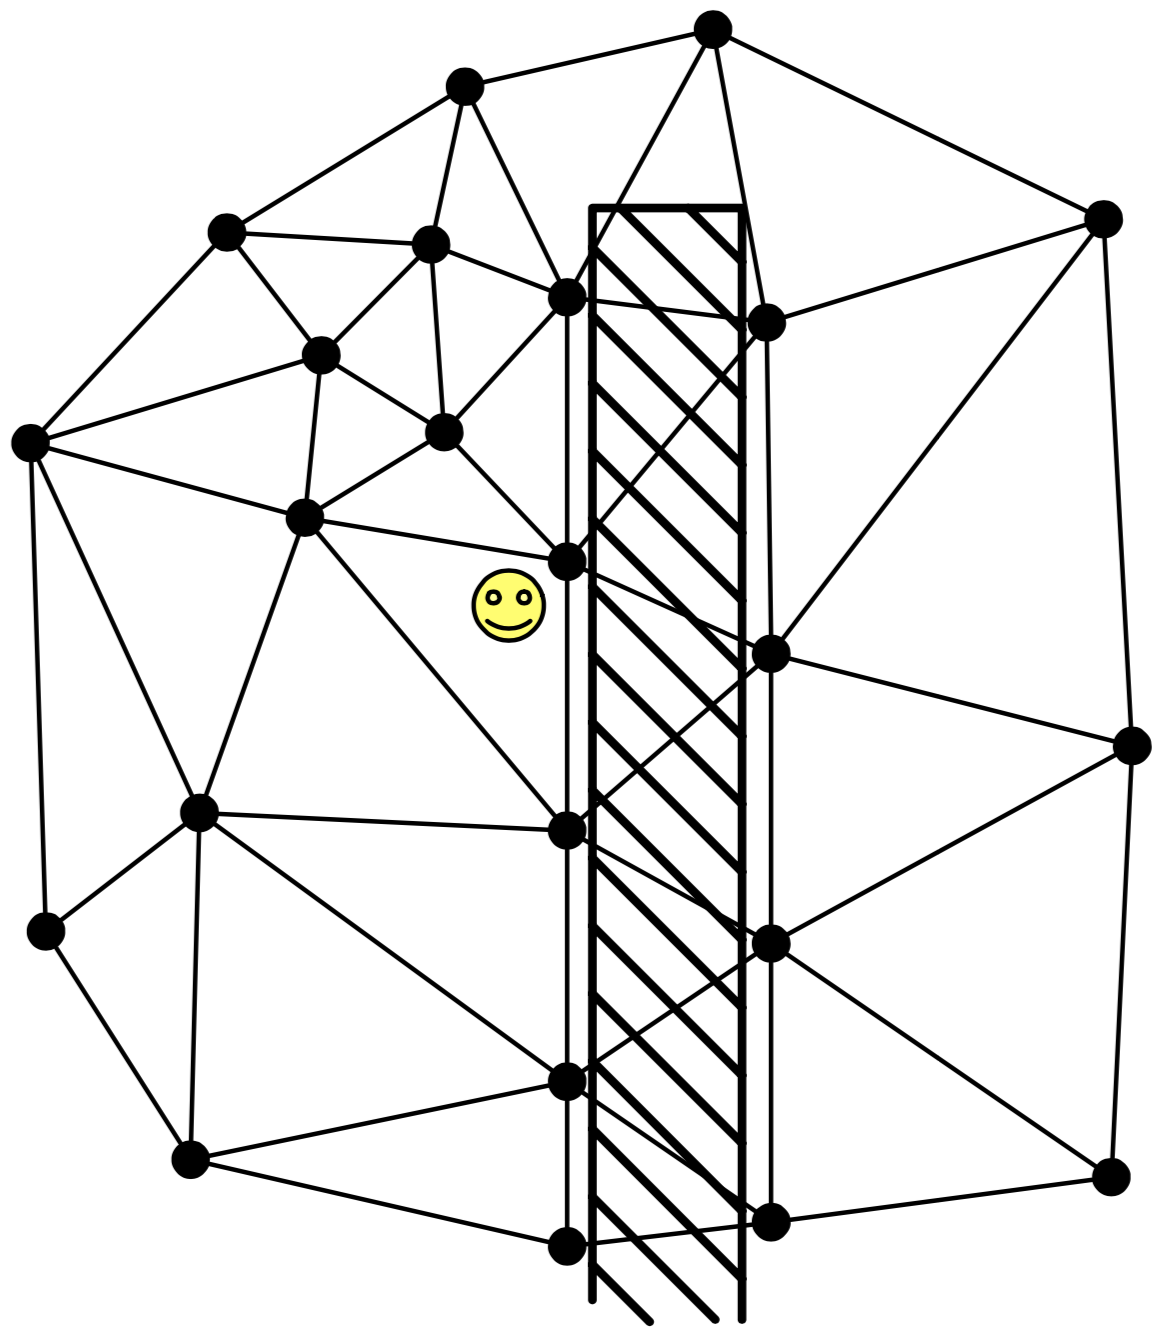
\includegraphics[width=0.45\textwidth]{figures/pl/key-points}
	\caption{由于能够任意放置体积光照样本的位置,因此这里首先在物体表面那些非连续区域放置一些关键位置,这就保证了空白空间中的像素始终会处于某4个合法体积光照样本构成的四面体内部(图片来自\cite{a:Lightprobeinterpolationusingtetrahedraltessellations})}
	\label{f:pl-key-points}
\end{figure}

在设置了这些关键位置之后,我们需要将这些样本位置连接起来形成一个由四面体构成的网格结构,这可以通过对网格执行约束德劳内四面体化(constrained Delaunay tetrahedralization)\mathindex{约束德劳内四面体化}{constrained Delaunay tetrahedralization}来实现。本书在前面第\ref{chp:rad}第\ref{sec:rad-triangulation}节介绍过约束德劳内三角化的知识,它通过对一个点集执行细分操作以形成一个三角形网格,并能够保证每个三角形的最小角最大化,因为最小角最大化能够使三角化的误差最小,这里的约束德劳内四面体化是类似的原理,它通过对已经标出重要性位置的点积执行四面体细分,并使得每个四面体内最小的立体角最大化。德劳内四面体化的场景如图\ref{f:pl-delaunay-tetrahedralisation}所示。

\begin{figure}
	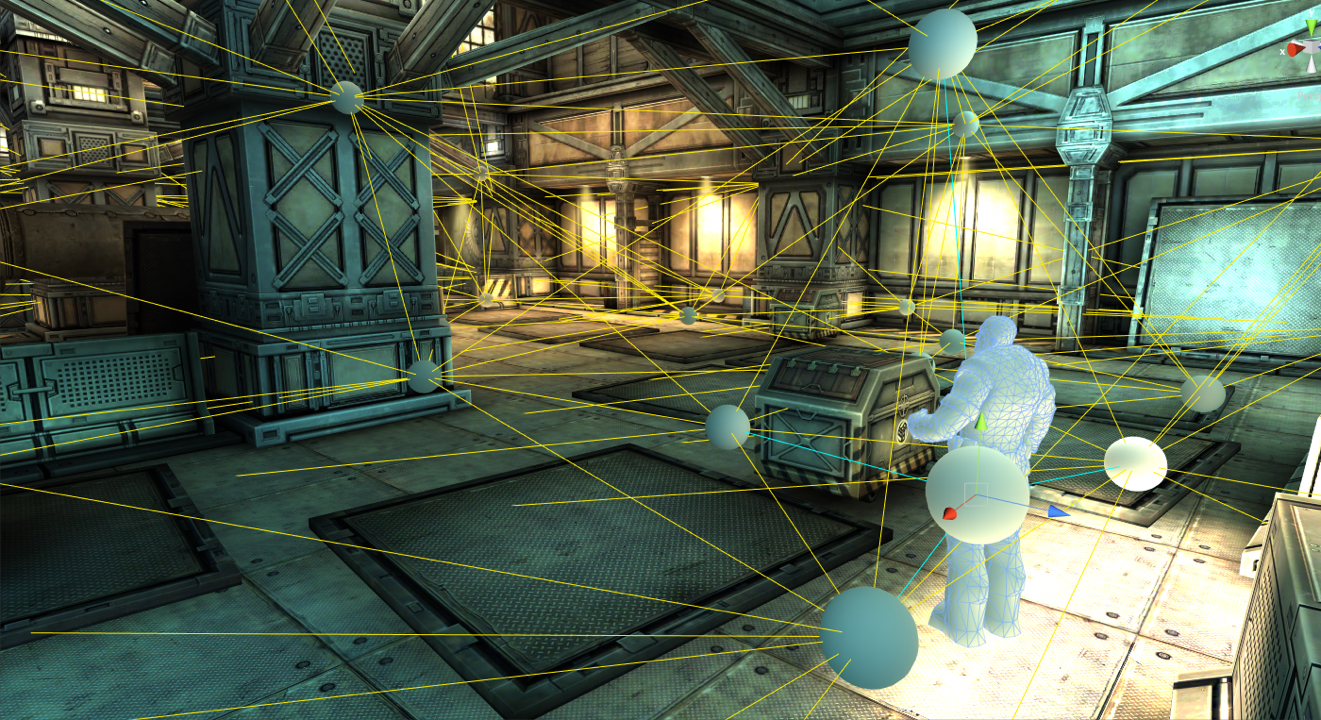
\includegraphics[width=\textwidth]{figures/pl/delaunay-tetrahedralisation}
	\caption{使用德劳内四面体化对场景的体积光照样本执行细分操作,这种细分的结果使体积光照样本的密度分布能够更好地适应场景的光照场变化(图片来自\cite{a:Lightprobeinterpolationusingtetrahedraltessellations})}
	\label{f:pl-delaunay-tetrahedralisation}
\end{figure}

尽管上述的过程看起来非常复杂,但是由于这些体积光照样本位置的构建是发生于预计算阶段,因此体积光照贴图的构建并不会给实时渲染带来压力。然而与样本结构的细分不同的是,查询一个像素位置位于哪个四面体的操作则是实时发生的,对四面体网格执行搜索相对于规则网格结构要复杂得多(例如规则网格可以通过简单的偏移来遍历所有的网格空间),在四面体网格中,四面体之间并不存在直接简单的空间关系,所以我们只有通过遍历所有四面体来搜索包含着色像素的四面体,但是为了减少重复的计算量,\cite{a:Leastsquaresconformalmapsforautomatictextureatlasgeneration}会保存动态物体上一帧所处的四面体索引,并通过存储四面体之间的相邻关系来减少对全局四面体网格的遍历,这里本书不在深入讨论,感兴趣的读者请前往原始论文。




\subsubsection{可见性}
尽管上面介绍的四面体插值方法避免了对非法体积光照样本的插值计算,但是它的代价也是非常高的,例如每个像素都要搜索整个四面体网格来寻找像素所在的四面体,尽管\cite{a:Lightprobeinterpolationusingtetrahedraltessellations}使用了一些缓存来避免了部分重复计算,但是相对于简单的规则网格,其每像素的计算还是相对比较复杂,本节我们将会讨论在传统的规则网格结构下对着色像素和体积光照样本之间的可见性进行判断,一次来间接避免规则网格结构中非法体积光照样本的情况。

在基于图像的光照技术中,我们假设入射环境光照与表面的位置无关,因此环境光照变成一个全局的数据,它只需要存储一份即可。然而在反射方程中,物体的遮挡关系确是一个局部的数据,它随着物体的变化而变化,因此如果我们要存储这样的信息,它将会占据非常可观的存储空间,所以在基于图像的光照技术中,我们通常直接忽略反射方程中的可见性分布,这样着色的时候环境贴图只需要与表面的BRDF分布函数进行相乘即可。这带来的后果就是由于缺乏对遮挡的考虑,物体表面的光照会显得平坦而没有立体感,因此环境遮挡通常被用于辅助基于图像的光照技术,环境遮挡通常只在屏幕空间(而不是物体空间)被考虑,我们将在后面的章节中介绍更多关于环境遮挡的内容。

当这种环境光照由全局转换到局部区域时,可见性的判断就变得更加重要,因为局部区域的环境光照变化会非常大,例如在图\ref{f:pl-reconstruction-comparation}中,隔着墙面的两个相邻体积光照样本之间的光照差异非常大,如果不进行可见性判断就会导致光照泄露,其中一个室内的光照泄露到另一个完全不同光照条件的室内环境去。除此之外,有前面的内容可知,如果采样的是规则的网格结构,则某些体积光照样本很可能位于物体内部或者场景之外,这形成包含非法颜色的体积光照样本,例如当角色靠近墙面时会变得非常暗,因为它混合了一个来自物体内部不含任何光照信息的体积光照样本。

\begin{figure}
\begin{fullwidth}
	\begin{subfigure}[b]{\thewidth}
		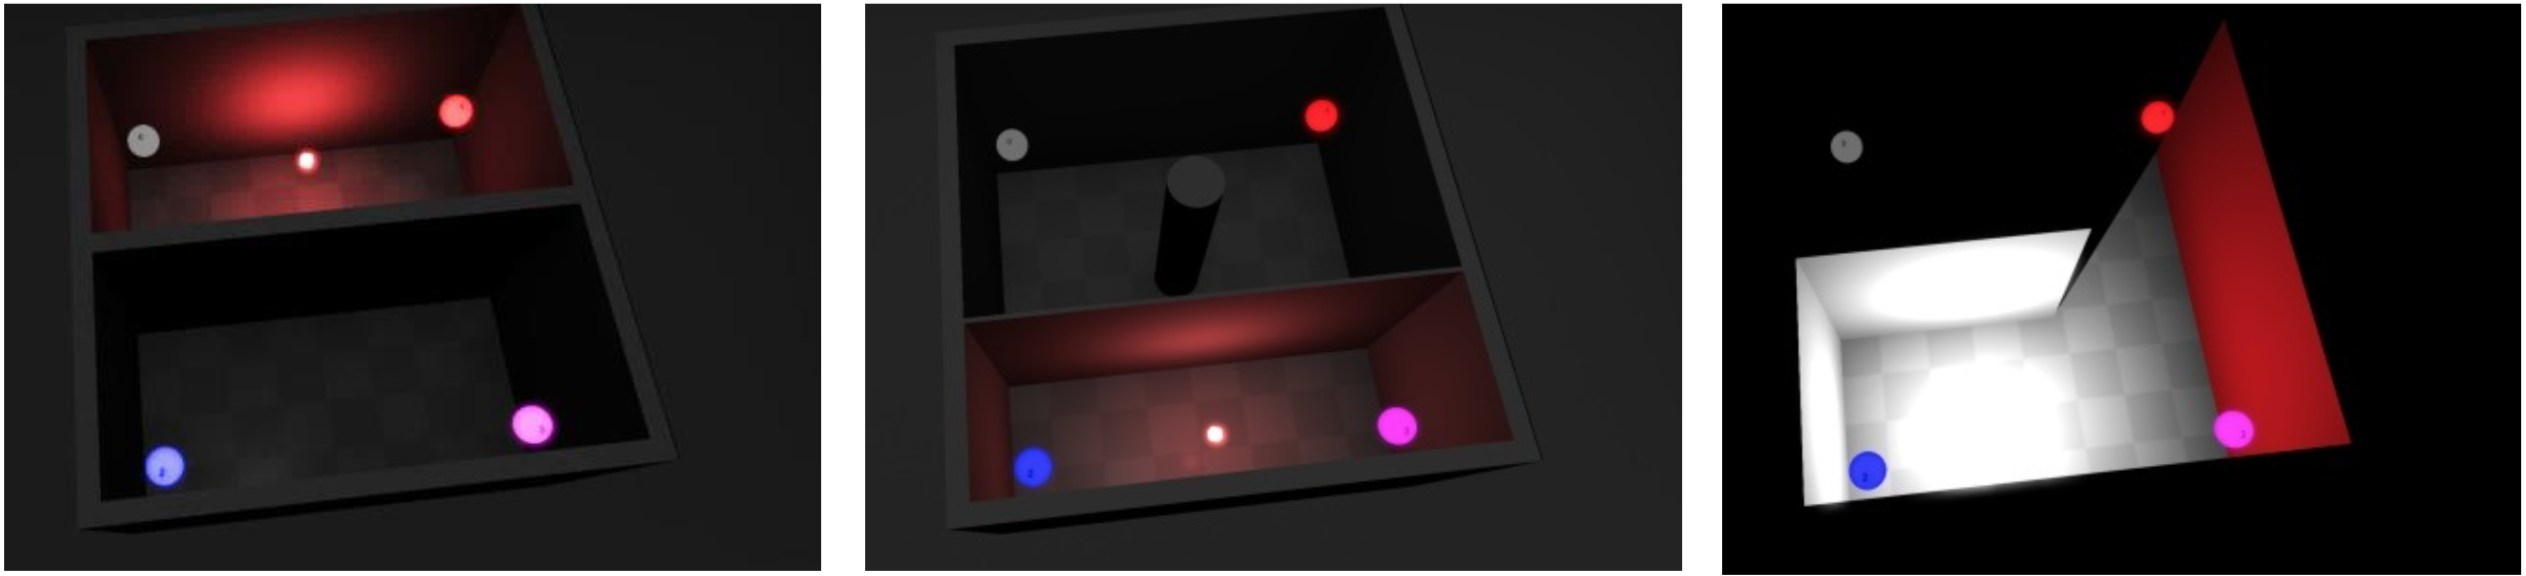
\includegraphics[width=\textwidth]{figures/pl/light-leaks-1}
		\caption{只包含直接光照的场景}
	\end{subfigure}
	\begin{subfigure}[b]{\thewidth}
		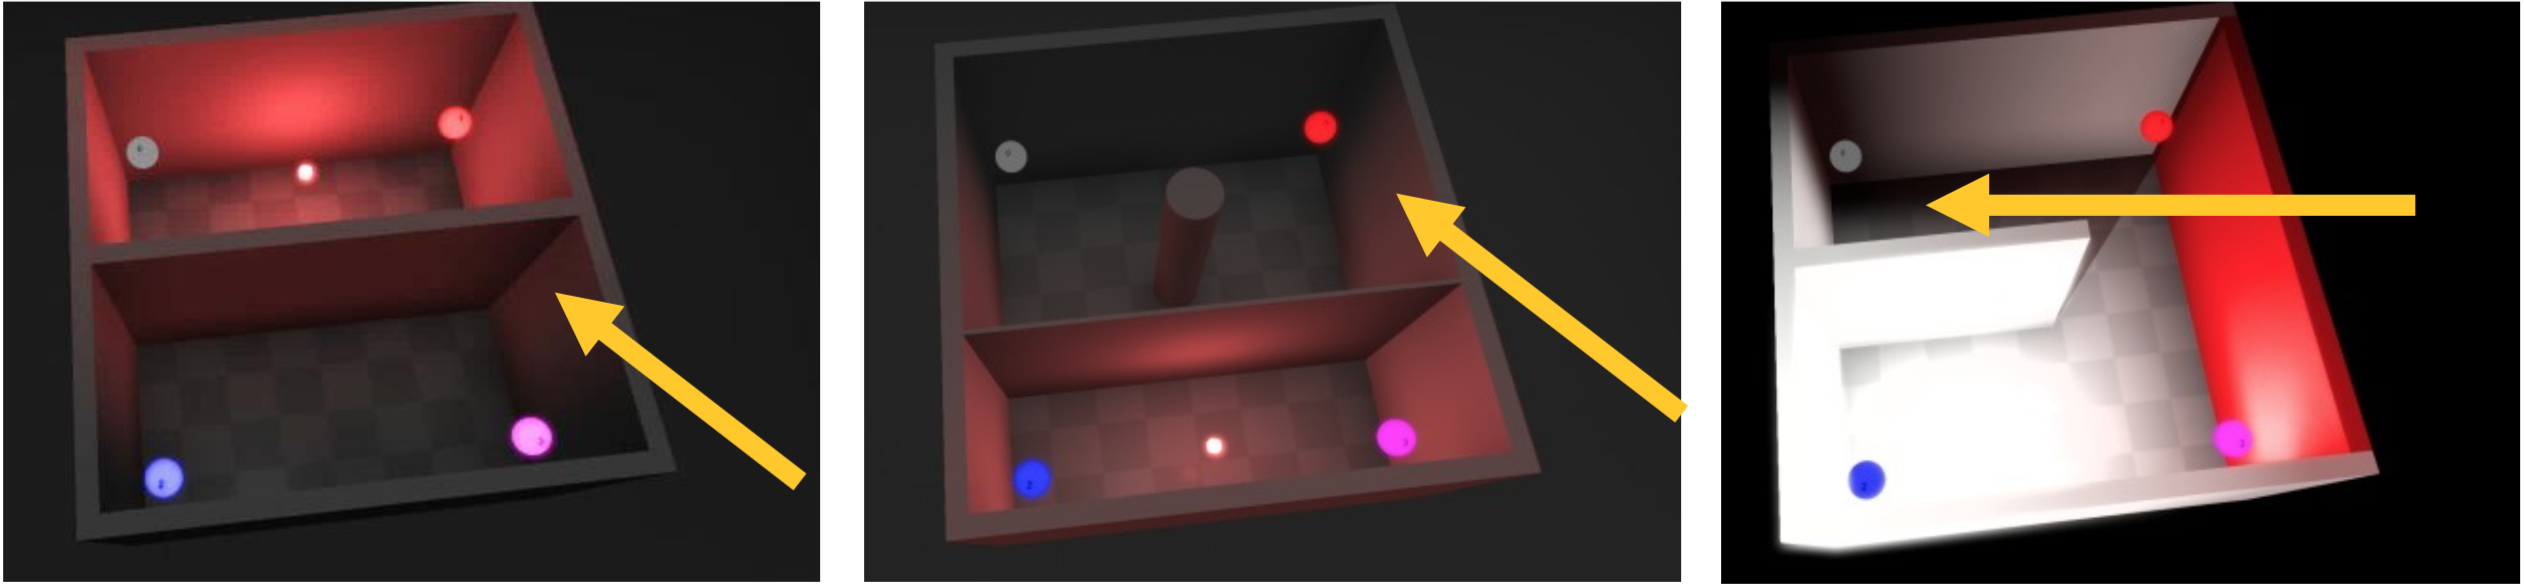
\includegraphics[width=\textwidth]{figures/pl/light-leaks-2}
			\caption{体积光照贴图的光照泄露}
	\end{subfigure}
	\begin{subfigure}[b]{\thewidth}
		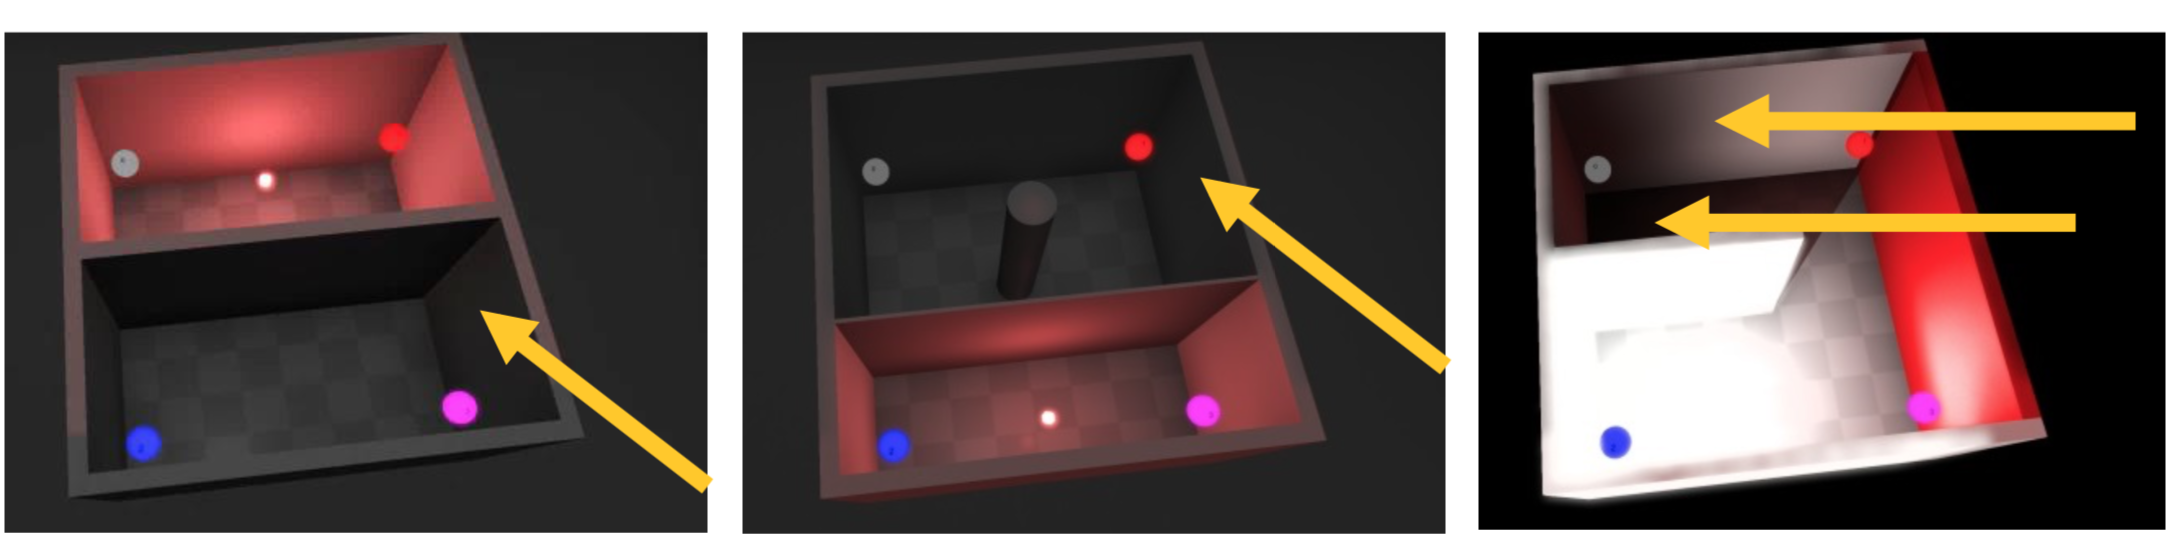
\includegraphics[width=\textwidth]{figures/pl/light-leaks-3}
			\caption{执行可见性判断的体积光照贴图效果}
	\end{subfigure}
	\caption{图中展示了三个简单的场景,其中(a)仅包含直接光照,由于直接光照包含可见性测试所以其结果是正确的,然而当使用体积光照贴图来计算间接光照时,由于缺乏可见性测试,两个相邻但是光照条件完全不同的场景之间就会出现光照泄露(b),在(c)中,通过简单地在体积光照样本和着色像素之间添加可见性测试,这种光照泄露可以被很好地控制(图片来自\cite{a:Lightprobeinterpolationusingtetrahedraltessellations})}
	\label{f:pl-reconstruction-comparation}
\end{fullwidth}
\end{figure}

本节我们将介绍一种来自\cite{a:Lightprobeinterpolationusingtetrahedraltessellations}的简单的可见性方法,该方法对每个体积光照样本存储一个深度图(实际上是使用一个双通道的纹理同时存储一个深度值,以及一个深度的平方值,我们将在后面介绍它们的用途),然后在实时渲染是通过对比着色像素到体积光照样本中心的距离与该方向的深度值来执行可见性判断,这个过程也即是一般阴影贴图的思路。

在实时渲染的时候,对每个体积光照样本除了考虑来自三线性插值得到的几何权重,还需要组合另外两个额外的权重值,其中第一个权重值是着色像素法线与着色像素至每个体积光照样本方向的点积,其结果会被限定为正。这个权重值的结果是产生一个平滑的背面剔除权重,例如如果着色像素的法线方向与该像素到体积光照样本的方向完全重合,这种情况就具有最大的权重系数1,随着这两个方向夹角的增加至$90^{\circ}$,其权重系数逐渐减小到0,当夹角大于$90^{\circ}$时,即表示光源位于物体背部,则其贡献值为0。

\begin{myshaded}
	使用一个平滑的余弦函数,而不仅仅是一个普通的背面剔除方法(例如0或者1)能够更好地近似辐射照度贴图对着色像素的光照贡献。思考传统漫反射表面的辐射亮度,它的光照是随着光线与法线夹角的变化而变化的,然而在对体积光照样本近似采样时,我只获取样本中一个确定方向的值,它并没有考虑这种着色像素的法线与两者之间光线的几何关系,所以这里的余弦函数正好是一个弥补。
\end{myshaded}

另一个额外的权重系数来源于着色像素与体积光照样本之间的可见性,这里仍然不是一个离散的可见性值,而是使用\cite{a:VarianceShadowMaps}提出的一个切比雪夫可见性测试结果,由于阴影贴图的频率变化非常大,传统的纹理过滤技术并不适合于对阴影贴图执行过滤,所以方差阴影贴图通过记录阴影贴图中每个像素局部区域的方差变化,来近似可见性测试,这里不再对其进行详述,感兴趣的读者请参考原文。

除此之外,在上述的方法中,体积光照样本的阴影贴图只记录了静态场景的深度值,因此它不能反映动态物体表面之间的自我遮挡关系,\cite{a:PrecomputedLightinginCallofDuty}提出了一种计算自我遮挡的可见性方法,这里也不再深入介绍。




\section{基于辐射亮度的预计算}
同局部的间接漫反射光照一样的道理,场景也需要局部的间接光泽反射光照,由于光泽反射是与观察方向有关的,因此它不能像辐射照度一样存储一个标量值,而是需要存储一个光照场,即空间中各个位置处的辐射亮度分布。

光照场(light field)\myindex{光照场}{light field},又称为全光函数(plenoptic function)\myindex{全光函数}{plenoptic function},它描述的是场景中空白空间中辐射亮度的空间和方向分布,它是一个5D的函数,其中三个维度用于表述空间的位置,另外两个维度用于表述辐射亮度的方向,它的概念最早出现于物理学文献中,最早于\cite{a:LightFieldRendering,a:Thelumigraph}中被引入到计算机图形学中,在这些方法中,光照场被使用一些离散空间样本表述,其中每个样本是一个辐射亮度的方向分布函数,我们称这个样本为一个光照场探针(light field probe)\myindex{光照场探针}{light field probe}。

光照场探针是和环境贴图类似的概念,即它收集来自环境各个方向的入射辐射亮度,因此光照场探针也可以使用立方体贴图,球谐函数等方向函数进行表述。光照场探针和环境贴图的主要区别是其接受来自周围环境入射光照的范围,环境贴图接受来自整个场景的反射光照,而光照场探针则主要收集来自某个局部空间的反射光照,通常我们需要对一个光照场探针指定一个几何包围盒,例如一个立方体或者球体。

在渲染的时候,对于光照场探针覆盖范围内的每一个着色点,我们假设它的入射光照分布都是相同的,即与位置无关的,因此该光照场探针作为表面着色点的入射光照分布,然后我们对表面执行一般的反射方程进行着色计算。

从上面的分析可以看出,光照场探针具有两个不足,首先它的光照分布与位置无关,这种假设对于全局的环境光照是比较精确的,因为着色像素通常离周围的环境很远,然而将这种概念放到局部时,着色像素离周围环境通常很近,因此这种假设带来的误差很大;其次环境光照通常是不考虑可见性的,然后使用一个全局的环境遮挡(ambient occlusion)来近似这种遮挡关系,然而在局部的区间内,我们需要更精确的可见性方法,我们将在本节后面讨论光照场探针的可见性测试。

针对第一个问题,它在光滑且平坦的表面上表现得特别明显,因为这些表面更能较清晰的呈现反射物体原有的形状,而这种形状由于与位置无关的假设而发生了形变,如图\ref{f:pl-reflection-issues}(c)所示;而这个问题在弯曲或者粗糙的表面上表现就会好得多,我们能够观察到来自环境的粗略反射光照,又不会受困于具体的反射光照的精度,如图\ref{f:pl-reflection-issues}(a)和(b)所示。所以在使用光照场探针的时候,为了得到更好的效果,待着色物体应该是比较粗糙,弯曲或者法线细节比较丰富的表面。

\begin{figure}
\begin{fullwidth}
	\begin{subfigure}[b]{0.33\thewidth}
		\includegraphics[width=\textwidth]{figures/pl/reflection-1}
		\caption{平滑且弯曲的表面}
	\end{subfigure}
	\begin{subfigure}[b]{0.33\thewidth}
		\includegraphics[width=\textwidth]{figures/pl/reflection-2}
			\caption{粗糙且平坦的表面}
	\end{subfigure}
	\begin{subfigure}[b]{0.33\thewidth}
		\includegraphics[width=\textwidth]{figures/pl/reflection-3}
			\caption{平滑且平坦的表面}
	\end{subfigure}
	\caption{由于环境光照与位置无关的假设,其在局部环境中会表现出比较大的误差,特别是在平坦而光滑的表面上会表现得特别明显(c),而粗糙(b)或者弯曲(a)的表面则会表现的好得多(图片来自\cite{m:ReflectionEnvironment})}
	\label{f:pl-reflection-issues}
\end{fullwidth}
\end{figure}

另一点关于光照场探针(或者局部环境贴图)需要注意的是,正是由于这种与位置有关的误差,光照场探针接收的仅仅是来自漫反射表面的反射光照,这一点是非常关键的,它也是后面我们讨论基于光线追踪的可见性方法的重要基础。由于光泽反射是严格与位置相关且光照分布的频率是非常高的,因此这会导致那些没有处于光照场探针中心位置的反射光照呈现比较严重的视觉误差。所以例如在Unreal Engine 4当中,光照场探针的生成需要位于光照贴图的预处理之后,因为这时场景才包含了间接漫反射光照,所以这也要求场景的表面主要是漫反射表面,光泽表面的场景其效果就要差得多,更多的信息可以参考\cite{m:ReflectionEnvironment}。

由于光照场探针记录的是入射辐射亮度,因此在着色的时候,我们需要将其与表面上余弦加权的BRDF函数相乘然后在半球空间上做积分计算,这对于实时渲染其成本是比较昂贵的。而由于辐射亮度相对于辐射照度分布更高的频率变化,它通常也不能使用低阶的球谐函数来近似,所以实时渲染中常见的做法仍然是对光照场探针执行预过滤操作,不同粗糙度的BRDF分布函数通常将其预过滤成不同分辨率的多级纹理,这样着色时的积分计算就被转化为一个纹理查询操作,这些内容和本章前面第\ref{sec:pl-pre-filtering}是一致的。这种基于预过滤的光照场探针技术在现代实时渲染中被大量使用,例如\cite{m:ReflectionEnvironment,m:LightProbes}。

最后我们再来总计一下光照场探针与体积光照样本两种技术在使用上的区别,如图\ref{f:pl-light-field}(b)所示,在空间中辐射亮度分布函数的频率变化通常是非常大的,它甚至存在非连续的边界导致其无限的频率分布,尽管预过滤的光照场探针其分布会平滑一些,但是它的频率变化仍然很高。因此在使用的时候,我们通常不会对多个光照场探针按空间进行插值计算(就像体积光照样本那样),而是每次使用单个光照场探针,并且将着色位置放置于探针中心来获取入射光照。由此可以看出,如果同一个环境存在多个光照场探针,这些探针通常不应该记录相同的环境\footnote{当然也可以对同一个环境放置多个探针,但是某些区域的光照场探针具有更高的分辨率来表现更精细的结构,当然它影响的范围可能更小,当物体移动到这个区域的时候,我们总是使用高分辨率的光照场探针。},因为我们只能选择使用一个,而只有当两个记录不同环境的光照场探针重合时,我们才能将两者的结果混合,否则可能相同的环境被反射两次,例如当角色从门口走向门外时,来自局部的光照场探针就应该和全局的环境贴图进行混合,因为它们两者记录的是完全不同的环境。

\begin{figure}
\begin{fullwidth}
	\begin{subfigure}[b]{0.33\thewidth}
		\includegraphics[width=\textwidth]{figures/pl/light-field-1}
		\caption{入射辐射亮度分布}
	\end{subfigure}
	\begin{subfigure}[b]{0.33\thewidth}
		\includegraphics[width=\textwidth]{figures/pl/light-field-2}
			\caption{光照场探针}
	\end{subfigure}
	\begin{subfigure}[b]{0.33\thewidth}
		\includegraphics[width=\textwidth]{figures/pl/light-field-3}
			\caption{体积光照样本}
	\end{subfigure}
	\caption{本图展示辐射亮度分布函数和辐射照度分布函数的差异,辐射亮度分布可能存在非连续的结构(b),因此其频率变化较大,通常不能使用如低阶的球谐函数来近似,而辐射照度因为对辐射亮度分布执行了半球空间内的过滤,因此其分布通常非常平滑(c),因此可以使用低阶的球谐函数来近似,注意(b)和(c)中箭头的距离表述了相应辐射亮度和辐射照度值的大小(图片来自\cite{a:TheIrradianceVolume})}
	\label{f:pl-light-field}
\end{fullwidth}
\end{figure}

而另一方面,辐射照度值在空间的变化要平滑得多,如图\ref{f:pl-light-field}(c)所示,因此我们可以通过插值计算来推断空间中每一个位置处的辐射照度值。所以可以看到,辐射亮度和辐射照度值的两种使用方式是非常不一样的,其着我们只在离散的位置计算,因此忽略了光照场探针内的位置,而后者则尝试通过插值重建整个空间的辐射照度分布。读者需要特别理解整个概念,对于光照场探针,我们并没有尝试重建整个空间的辐射亮度分布。




\subsection{基于光线追踪的方法}
光照场探针和体积光照贴图都是基于图像的光照技术(参见第\ref{sec:pl-ibl}节),(特别是在实时渲染中)基于图像的光照技术通常会忽略直接的可见性计算,转而使用一些其它方法来对可见性进行近似处理,例如使用一个粗略的环境遮挡,或者如上一节介绍的仅仅考虑着色点与体积光照样本之间的可见性,而忽略表面内部的自我遮挡等。

为了更好地理解光照场探针和体积光照贴图的概念,以及其涉及的可见性问题,我们来重新分析一下表面的反射方程:

\begin{equation}
	L_o(\omega_o)=\int_{\Omega}L_i(\omega_i)f_r(\omega_i,\omega_o)V(\omega_i)\cos(\omega_i,\mathbf{n}){\rm d}\omega_i
\end{equation}

对于上述着色方程,在基于图像的光照技术中$L_i(\omega_i)$表述为环境贴图,然后为避免实时渲染时的昂贵积分计算,环境贴图通常被BRDF分布函数$f_r(\omega_i,\omega_o)$执行预过滤并存储在多级环境贴图的形式,而可见性函数$V(\omega_i)$被忽略。

可以看到,可见性函数是与入射方向有关的,所以上面提到的这些可见性的近似方法并不是很准确,例如环境遮挡并不会考虑入射光的方向分布;而可见性函数$V(\omega_i)$对预过滤中的每一个样本都是有影响的,所以在预过滤的时候忽略这种可见性影响,而在之后单一地判断着色像素与体积光照样本之间可见性的方法也不是很准确;\cite{a:PrecomputedLightinginCallofDuty}尝试考虑可见性函数的方向性分布,是一种相对比较精确的可见性方法。

那么要怎样更好地考虑环境贴图的可见性呢?答案是使用基于光线追踪的方法,本节我们将介绍\cite{a:Real-TimeGlobalIlluminationusingPrecomputedLightFieldProbes}提供的一种方法。

首先需要明白的是,为了精确考虑着色像素与光源之间的可见性,就不能对光照场探针(或环境贴图)使用预过滤,因为预过滤的部分仅包含BRDF分布函数,而不包含可见性函数,我们无法通过任何手段能够从预过滤后的光照重建出比较准确的可见性关系,所以在本节介绍的方法中我们需要直接在原始的环境贴图上进行计算。

\begin{figure}
\begin{fullwidth}
	\includegraphics[width=\thewidth]{figures/pl/light-field-probes}
	\caption{一个光照探针的表述:入射辐射亮度(左),法线(中)以及距离(右)贴图,所有的方向信息都被映射到一个八面体贴图中(图片来自\cite{a:Real-TimeGlobalIlluminationusingPrecomputedLightFieldProbes})}
	\label{f:pl-light-field-probes}
\end{fullwidth}
\end{figure}

那么在不使用预过滤的情况下,应该怎样高效地计算反射方程所表述的积分呢?在\cite{a:Real-TimeGlobalIlluminationusingPrecomputedLightFieldProbes}中,光照场探针首先被表述为如下的数据结构\cite{a:ALightFieldRepresentationforRealTimeGlobalIllumination}(其中每个类型的数据就被映射到一个八面体上):

\begin{itemize}
	\item 该光照场探针中心位置处的入射辐射亮度,如图\ref{f:pl-light-field-probes}左边小图所示,通过前面的内容分析可知,这些入射光照来自于周围的漫反射表面。
	\item 每个入射光照所在表面的法线,如图\ref{f:pl-light-field-probes}中间小图所示。
	\item 光照场探针中心到每个入射光照方向上最近表面的距离,如图\ref{f:pl-light-field-probes}右边小图所示。
\end{itemize}

有了上述这些信息,由于我们只需要计算那些对于摄像机可见的像素的间接光照,所以我们可以对所有屏幕空间的像素执行光线追踪计算,不过这里的光线追踪并不是针对几何场景,而是对所有的光照场探针。由于光照场探针的深度贴图保持了场景的几何信息以及这些几何表面的漫反射颜色值,所有如果我们只要找到每个光线与光照场探针的深度贴图相交的位置,那么我们就能取得该光线方向上的入射光照。

那么应该怎样执行光线与一个光照场探针的光线追踪呢?\cite{a:ALightFieldRepresentationforRealTimeGlobalIllumination}发现,由于八面体映射具有比较好的线性关系,所以当一个世界空间的光线投影到八面体贴图上时,其结果是一个分段的线性直线线段,因此这种世界空间的光线追踪就被转化为八面体贴图上的像素遍历操作,并且这些分段直线在八面体贴图上是相连的,如图\ref{f:pl-single-probe-ray-tracing}所示。

\begin{figure}
	\includegraphics[width=\textwidth]{figures/pl/single-probe-ray-tracing}
	\caption{单个光照场探针的光线追踪,其中一条空间的光线被映射为八面体贴图空间上几个分段的直线,这些直线段之间在八面体的边缘是相连的,\cite{a:Real-TimeGlobalIlluminationusingPrecomputedLightFieldProbes}对每个光照场探针使用了两个分辨率的贴图,其中低分辨率的贴图用来加速那些空白空间的光线步进,如图中的黄色箭头所示,而绿色箭头表示在高分辨率的八面体贴图中步进(图片来自\cite{a:Real-TimeGlobalIlluminationusingPrecomputedLightFieldProbes})}
	\label{f:pl-single-probe-ray-tracing}
\end{figure}

采用上述的方法,对于一条光线,我们到底要怎样取得该光线上的辐射亮度值呢?本章前面已经反复强调,光照场探针存储的是来自漫反射表面的入射辐射亮度值,因此我们只需要找到光线与光照场探针的深度图的交点,直接读取该交点处光照场探针在该方向的入射辐射亮度值即可,因为该点是漫反射表面,它向任何方向反射的光照都是一样的。

在图\ref{f:pl-light-field-ray-marching}中,外面的凸形几何形状表示光照场探针${\rm P}$的深度图,现在我们需要求点${\rm X}$处沿$\omega$方向的间接光照,我们首先让光线在$\omega$方向上步进,根据前面介绍的内容,这仅仅涉及到在屏幕空间的像素遍历而已,在光线步进中,我们不断将当前步进位置到${\rm P}$的距离与${\rm P}$沿该方向上的深度值进行比较,如果这两个值非常接近,则我们可以认为找到了光线与光照场探针的一个焦点,我们去该交点处光照场的颜色值即可。

\begin{figure}
	\sidecaption
	\includegraphics[width=0.5\textwidth]{figures/pl/light-field-ray-marching}
	\caption{光照场接受的是来自漫反射表面的光照,所以只要找到光线与光照场深度图上的一个交点,则光照场探针在该交点对应的辐射亮度就可以用作为光线的入射辐射亮度}
	\label{f:pl-light-field-ray-marching}
\end{figure}

当然\cite{a:Real-TimeGlobalIlluminationusingPrecomputedLightFieldProbes}的观察主要是基于光照场探针对应的几何环境是一个凸面体形状,如果环境保护太多细节,那么光线与光照场探针的相交测试就可能会失败,其解决的方法就是使用多个光照场探针,这些相邻的光照场探针会重复记录周围的场景,并且不同位置的光照场探针分布能够很好地使用场景的几何分布,因此只要光照场探针的密度足够高,这种相交测试的精确度就会更高。

所以,光线对整个光照场的光线追踪就涉及到两个步骤,首先是选择一个光照场探针,然后是对每个选择的光照场探针执行上述的光线追踪计算,如果当前的光照场探针没有找到相交点,则继续选择下一个光照场探针继续执行上述的操作,如果光线在某个光照场探针内找到相交点,则直接从该光照场读取相应的辐射亮度值。其中\cite{a:LightProbeSelectionAlgorithmsforReal-TimeRenderingofLightFields}提出了种光照场探针的选择算法,是可以加速找到光线与光照场探针的相交点,这里不再详述。

最后,有了上述的光线追踪方法,我们能够得到屏幕上每个像素任意方向上的入射光照,那么应该怎样计算最终像素的间接漫反射和光照反射光照呢?\cite{a:Real-TimeGlobalIlluminationusingPrecomputedLightFieldProbes}的方法是对每个像素的漫反射和BRDF分布函数分别进行一次采样,然后对所有像素得到的图像分布进行降噪处理,最终就可以得到每个可见像素的间接漫反射和间接光泽反射光照。

当然,由于漫反射BRDF涉及的采样范围很大,因此每个像素仅使用单个样本会导致比较大的方差,所以对于漫反射我们仍然可以选择使用前面介绍的预过滤方法。

我们可以看到,这种方法将漫反射和光照反射统一对待,它也不会对原始光照场探针执行任何的预过滤操作,并且它移除了基于图像的光照中与位置无关的假设,每个光线都是接受的来自真实位置的入射光照,而其中的光照场探针(或环境贴图)变成一个用于辅助光线追踪的数据结构。